% Options for packages loaded elsewhere
\PassOptionsToPackage{unicode}{hyperref}
\PassOptionsToPackage{hyphens}{url}
%
\documentclass[
]{book}
\usepackage{amsmath,amssymb}
\usepackage{lmodern}
\usepackage{iftex}
\ifPDFTeX
  \usepackage[T1]{fontenc}
  \usepackage[utf8]{inputenc}
  \usepackage{textcomp} % provide euro and other symbols
\else % if luatex or xetex
  \usepackage{unicode-math}
  \defaultfontfeatures{Scale=MatchLowercase}
  \defaultfontfeatures[\rmfamily]{Ligatures=TeX,Scale=1}
\fi
% Use upquote if available, for straight quotes in verbatim environments
\IfFileExists{upquote.sty}{\usepackage{upquote}}{}
\IfFileExists{microtype.sty}{% use microtype if available
  \usepackage[]{microtype}
  \UseMicrotypeSet[protrusion]{basicmath} % disable protrusion for tt fonts
}{}
\makeatletter
\@ifundefined{KOMAClassName}{% if non-KOMA class
  \IfFileExists{parskip.sty}{%
    \usepackage{parskip}
  }{% else
    \setlength{\parindent}{0pt}
    \setlength{\parskip}{6pt plus 2pt minus 1pt}}
}{% if KOMA class
  \KOMAoptions{parskip=half}}
\makeatother
\usepackage{xcolor}
\usepackage{color}
\usepackage{fancyvrb}
\newcommand{\VerbBar}{|}
\newcommand{\VERB}{\Verb[commandchars=\\\{\}]}
\DefineVerbatimEnvironment{Highlighting}{Verbatim}{commandchars=\\\{\}}
% Add ',fontsize=\small' for more characters per line
\usepackage{framed}
\definecolor{shadecolor}{RGB}{248,248,248}
\newenvironment{Shaded}{\begin{snugshade}}{\end{snugshade}}
\newcommand{\AlertTok}[1]{\textcolor[rgb]{0.94,0.16,0.16}{#1}}
\newcommand{\AnnotationTok}[1]{\textcolor[rgb]{0.56,0.35,0.01}{\textbf{\textit{#1}}}}
\newcommand{\AttributeTok}[1]{\textcolor[rgb]{0.77,0.63,0.00}{#1}}
\newcommand{\BaseNTok}[1]{\textcolor[rgb]{0.00,0.00,0.81}{#1}}
\newcommand{\BuiltInTok}[1]{#1}
\newcommand{\CharTok}[1]{\textcolor[rgb]{0.31,0.60,0.02}{#1}}
\newcommand{\CommentTok}[1]{\textcolor[rgb]{0.56,0.35,0.01}{\textit{#1}}}
\newcommand{\CommentVarTok}[1]{\textcolor[rgb]{0.56,0.35,0.01}{\textbf{\textit{#1}}}}
\newcommand{\ConstantTok}[1]{\textcolor[rgb]{0.00,0.00,0.00}{#1}}
\newcommand{\ControlFlowTok}[1]{\textcolor[rgb]{0.13,0.29,0.53}{\textbf{#1}}}
\newcommand{\DataTypeTok}[1]{\textcolor[rgb]{0.13,0.29,0.53}{#1}}
\newcommand{\DecValTok}[1]{\textcolor[rgb]{0.00,0.00,0.81}{#1}}
\newcommand{\DocumentationTok}[1]{\textcolor[rgb]{0.56,0.35,0.01}{\textbf{\textit{#1}}}}
\newcommand{\ErrorTok}[1]{\textcolor[rgb]{0.64,0.00,0.00}{\textbf{#1}}}
\newcommand{\ExtensionTok}[1]{#1}
\newcommand{\FloatTok}[1]{\textcolor[rgb]{0.00,0.00,0.81}{#1}}
\newcommand{\FunctionTok}[1]{\textcolor[rgb]{0.00,0.00,0.00}{#1}}
\newcommand{\ImportTok}[1]{#1}
\newcommand{\InformationTok}[1]{\textcolor[rgb]{0.56,0.35,0.01}{\textbf{\textit{#1}}}}
\newcommand{\KeywordTok}[1]{\textcolor[rgb]{0.13,0.29,0.53}{\textbf{#1}}}
\newcommand{\NormalTok}[1]{#1}
\newcommand{\OperatorTok}[1]{\textcolor[rgb]{0.81,0.36,0.00}{\textbf{#1}}}
\newcommand{\OtherTok}[1]{\textcolor[rgb]{0.56,0.35,0.01}{#1}}
\newcommand{\PreprocessorTok}[1]{\textcolor[rgb]{0.56,0.35,0.01}{\textit{#1}}}
\newcommand{\RegionMarkerTok}[1]{#1}
\newcommand{\SpecialCharTok}[1]{\textcolor[rgb]{0.00,0.00,0.00}{#1}}
\newcommand{\SpecialStringTok}[1]{\textcolor[rgb]{0.31,0.60,0.02}{#1}}
\newcommand{\StringTok}[1]{\textcolor[rgb]{0.31,0.60,0.02}{#1}}
\newcommand{\VariableTok}[1]{\textcolor[rgb]{0.00,0.00,0.00}{#1}}
\newcommand{\VerbatimStringTok}[1]{\textcolor[rgb]{0.31,0.60,0.02}{#1}}
\newcommand{\WarningTok}[1]{\textcolor[rgb]{0.56,0.35,0.01}{\textbf{\textit{#1}}}}
\usepackage{longtable,booktabs,array}
\usepackage{calc} % for calculating minipage widths
% Correct order of tables after \paragraph or \subparagraph
\usepackage{etoolbox}
\makeatletter
\patchcmd\longtable{\par}{\if@noskipsec\mbox{}\fi\par}{}{}
\makeatother
% Allow footnotes in longtable head/foot
\IfFileExists{footnotehyper.sty}{\usepackage{footnotehyper}}{\usepackage{footnote}}
\makesavenoteenv{longtable}
\usepackage{graphicx}
\makeatletter
\def\maxwidth{\ifdim\Gin@nat@width>\linewidth\linewidth\else\Gin@nat@width\fi}
\def\maxheight{\ifdim\Gin@nat@height>\textheight\textheight\else\Gin@nat@height\fi}
\makeatother
% Scale images if necessary, so that they will not overflow the page
% margins by default, and it is still possible to overwrite the defaults
% using explicit options in \includegraphics[width, height, ...]{}
\setkeys{Gin}{width=\maxwidth,height=\maxheight,keepaspectratio}
% Set default figure placement to htbp
\makeatletter
\def\fps@figure{htbp}
\makeatother
\setlength{\emergencystretch}{3em} % prevent overfull lines
\providecommand{\tightlist}{%
  \setlength{\itemsep}{0pt}\setlength{\parskip}{0pt}}
\setcounter{secnumdepth}{5}
\newlength{\cslhangindent}
\setlength{\cslhangindent}{1.5em}
\newlength{\csllabelwidth}
\setlength{\csllabelwidth}{3em}
\newlength{\cslentryspacingunit} % times entry-spacing
\setlength{\cslentryspacingunit}{\parskip}
\newenvironment{CSLReferences}[2] % #1 hanging-ident, #2 entry spacing
 {% don't indent paragraphs
  \setlength{\parindent}{0pt}
  % turn on hanging indent if param 1 is 1
  \ifodd #1
  \let\oldpar\par
  \def\par{\hangindent=\cslhangindent\oldpar}
  \fi
  % set entry spacing
  \setlength{\parskip}{#2\cslentryspacingunit}
 }%
 {}
\usepackage{calc}
\newcommand{\CSLBlock}[1]{#1\hfill\break}
\newcommand{\CSLLeftMargin}[1]{\parbox[t]{\csllabelwidth}{#1}}
\newcommand{\CSLRightInline}[1]{\parbox[t]{\linewidth - \csllabelwidth}{#1}\break}
\newcommand{\CSLIndent}[1]{\hspace{\cslhangindent}#1}
\usepackage{booktabs}
\usepackage{longtable}
\usepackage{array}
\usepackage{multirow}
\usepackage{wrapfig}
\usepackage{float}
\usepackage{colortbl}
\usepackage{pdflscape}
\usepackage{tabu}
\usepackage{threeparttable}
\usepackage{threeparttablex}
\usepackage[normalem]{ulem}
\usepackage{makecell}
\usepackage{xcolor}
\usepackage{multicol}
\usepackage{hhline}
\newlength\Oldarrayrulewidth
\newlength\Oldtabcolsep
\usepackage{hyperref}
\usepackage{amsmath}
\usepackage{caption}
\ifLuaTeX
  \usepackage{selnolig}  % disable illegal ligatures
\fi
\IfFileExists{bookmark.sty}{\usepackage{bookmark}}{\usepackage{hyperref}}
\IfFileExists{xurl.sty}{\usepackage{xurl}}{} % add URL line breaks if available
\urlstyle{same} % disable monospaced font for URLs
\hypersetup{
  pdftitle={Greenhouse Gas Emissions Scenario Planning},
  pdfauthor={Metropolitan Council},
  hidelinks,
  pdfcreator={LaTeX via pandoc}}

\title{Greenhouse Gas Emissions Scenario Planning}
\author{Metropolitan Council}
\date{February 2023}

\begin{document}
\maketitle

{
\setcounter{tocdepth}{1}
\tableofcontents
}
\hypertarget{section}{%
\chapter*{}\label{section}}
\addcontentsline{toc}{chapter}{}

\includegraphics{../images/2788.jpg}

\hypertarget{metropolitan-council}{%
\section*{Metropolitan Council}\label{metropolitan-council}}
\addcontentsline{toc}{section}{Metropolitan Council}

\begin{center}\rule{0.5\linewidth}{0.5pt}\end{center}

\begin{verbatim}
## Warning: fonts used in `flextable` are ignored because the `pdflatex` engine
## is used and not `xelatex` or `lualatex`. You can avoid this warning by using
## the `set_flextable_defaults(fonts_ignore=TRUE)` command or use a compatible
## engine by defining `latex_engine: xelatex` in the YAML header of the R Markdown
## document.
\end{verbatim}

\global\setlength{\Oldarrayrulewidth}{\arrayrulewidth}

\global\setlength{\Oldtabcolsep}{\tabcolsep}

\setlength{\tabcolsep}{0pt}

\renewcommand*{\arraystretch}{1.5}



\providecommand{\ascline}[3]{\noalign{\global\arrayrulewidth #1}\arrayrulecolor[HTML]{#2}\cline{#3}}

\begin{longtable}[c]{|p{1.76in}|p{0.88in}|p{1.80in}|p{0.96in}}





\multicolumn{1}{>{\raggedright}p{\dimexpr 1.76in+0\tabcolsep}}{\textcolor[HTML]{000000}{\fontsize{9}{9}\selectfont{Charlie\ Zelle}}} & \multicolumn{1}{>{\raggedright}p{\dimexpr 0.88in+0\tabcolsep}}{\textcolor[HTML]{000000}{\fontsize{9}{9}\selectfont{Chair}}} & \multicolumn{1}{>{\raggedright}p{\dimexpr 1.8in+0\tabcolsep}}{\textcolor[HTML]{000000}{\fontsize{9}{9}\selectfont{Raymond\ Zeran}}} & \multicolumn{1}{>{\raggedright}p{\dimexpr 0.96in+0\tabcolsep}}{\textcolor[HTML]{000000}{\fontsize{9}{9}\selectfont{District\ 9}}} \\





\multicolumn{1}{>{\raggedright}p{\dimexpr 1.76in+0\tabcolsep}}{\textcolor[HTML]{000000}{\fontsize{9}{9}\selectfont{Judy\ Johnson}}} & \multicolumn{1}{>{\raggedright}p{\dimexpr 0.88in+0\tabcolsep}}{\textcolor[HTML]{000000}{\fontsize{9}{9}\selectfont{District\ 1}}} & \multicolumn{1}{>{\raggedright}p{\dimexpr 1.8in+0\tabcolsep}}{\textcolor[HTML]{000000}{\fontsize{9}{9}\selectfont{Peter\ Lindstrom}}} & \multicolumn{1}{>{\raggedright}p{\dimexpr 0.96in+0\tabcolsep}}{\textcolor[HTML]{000000}{\fontsize{9}{9}\selectfont{District\ 10}}} \\





\multicolumn{1}{>{\raggedright}p{\dimexpr 1.76in+0\tabcolsep}}{\textcolor[HTML]{000000}{\fontsize{9}{9}\selectfont{Reva\ Chamblis}}} & \multicolumn{1}{>{\raggedright}p{\dimexpr 0.88in+0\tabcolsep}}{\textcolor[HTML]{000000}{\fontsize{9}{9}\selectfont{District\ 2}}} & \multicolumn{1}{>{\raggedright}p{\dimexpr 1.8in+0\tabcolsep}}{\textcolor[HTML]{000000}{\fontsize{9}{9}\selectfont{Susan\ Vento}}} & \multicolumn{1}{>{\raggedright}p{\dimexpr 0.96in+0\tabcolsep}}{\textcolor[HTML]{000000}{\fontsize{9}{9}\selectfont{District\ 11}}} \\





\multicolumn{1}{>{\raggedright}p{\dimexpr 1.76in+0\tabcolsep}}{\textcolor[HTML]{000000}{\fontsize{9}{9}\selectfont{Christopher\ Ferguson}}} & \multicolumn{1}{>{\raggedright}p{\dimexpr 0.88in+0\tabcolsep}}{\textcolor[HTML]{000000}{\fontsize{9}{9}\selectfont{District\ 3}}} & \multicolumn{1}{>{\raggedright}p{\dimexpr 1.8in+0\tabcolsep}}{\textcolor[HTML]{000000}{\fontsize{9}{9}\selectfont{Francisco\ J.\ Gonzalez}}} & \multicolumn{1}{>{\raggedright}p{\dimexpr 0.96in+0\tabcolsep}}{\textcolor[HTML]{000000}{\fontsize{9}{9}\selectfont{District\ 12}}} \\





\multicolumn{1}{>{\raggedright}p{\dimexpr 1.76in+0\tabcolsep}}{\textcolor[HTML]{000000}{\fontsize{9}{9}\selectfont{Deb\ Barber}}} & \multicolumn{1}{>{\raggedright}p{\dimexpr 0.88in+0\tabcolsep}}{\textcolor[HTML]{000000}{\fontsize{9}{9}\selectfont{District\ 4}}} & \multicolumn{1}{>{\raggedright}p{\dimexpr 1.8in+0\tabcolsep}}{\textcolor[HTML]{000000}{\fontsize{9}{9}\selectfont{Chai\ Lee}}} & \multicolumn{1}{>{\raggedright}p{\dimexpr 0.96in+0\tabcolsep}}{\textcolor[HTML]{000000}{\fontsize{9}{9}\selectfont{District\ 13}}} \\





\multicolumn{1}{>{\raggedright}p{\dimexpr 1.76in+0\tabcolsep}}{\textcolor[HTML]{000000}{\fontsize{9}{9}\selectfont{Molly\ Cummings}}} & \multicolumn{1}{>{\raggedright}p{\dimexpr 0.88in+0\tabcolsep}}{\textcolor[HTML]{000000}{\fontsize{9}{9}\selectfont{District\ 5}}} & \multicolumn{1}{>{\raggedright}p{\dimexpr 1.8in+0\tabcolsep}}{\textcolor[HTML]{000000}{\fontsize{9}{9}\selectfont{Kris\ Fredson}}} & \multicolumn{1}{>{\raggedright}p{\dimexpr 0.96in+0\tabcolsep}}{\textcolor[HTML]{000000}{\fontsize{9}{9}\selectfont{District\ 14}}} \\





\multicolumn{1}{>{\raggedright}p{\dimexpr 1.76in+0\tabcolsep}}{\textcolor[HTML]{000000}{\fontsize{9}{9}\selectfont{John\ Pacheco\ Jr.}}} & \multicolumn{1}{>{\raggedright}p{\dimexpr 0.88in+0\tabcolsep}}{\textcolor[HTML]{000000}{\fontsize{9}{9}\selectfont{District\ 6}}} & \multicolumn{1}{>{\raggedright}p{\dimexpr 1.8in+0\tabcolsep}}{\textcolor[HTML]{000000}{\fontsize{9}{9}\selectfont{Phillip\ Sterner}}} & \multicolumn{1}{>{\raggedright}p{\dimexpr 0.96in+0\tabcolsep}}{\textcolor[HTML]{000000}{\fontsize{9}{9}\selectfont{District\ 15}}} \\





\multicolumn{1}{>{\raggedright}p{\dimexpr 1.76in+0\tabcolsep}}{\textcolor[HTML]{000000}{\fontsize{9}{9}\selectfont{Robert\ Lilligren}}} & \multicolumn{1}{>{\raggedright}p{\dimexpr 0.88in+0\tabcolsep}}{\textcolor[HTML]{000000}{\fontsize{9}{9}\selectfont{District\ 7}}} & \multicolumn{1}{>{\raggedright}p{\dimexpr 1.8in+0\tabcolsep}}{\textcolor[HTML]{000000}{\fontsize{9}{9}\selectfont{Wendy\ Wulff}}} & \multicolumn{1}{>{\raggedright}p{\dimexpr 0.96in+0\tabcolsep}}{\textcolor[HTML]{000000}{\fontsize{9}{9}\selectfont{District\ 16}}} \\





\multicolumn{1}{>{\raggedright}p{\dimexpr 1.76in+0\tabcolsep}}{\textcolor[HTML]{000000}{\fontsize{9}{9}\selectfont{Abdirahman\ Muse}}} & \multicolumn{1}{>{\raggedright}p{\dimexpr 0.88in+0\tabcolsep}}{\textcolor[HTML]{000000}{\fontsize{9}{9}\selectfont{District\ 8}}} & \multicolumn{1}{>{\raggedright}p{\dimexpr 1.8in+0\tabcolsep}}{\textcolor[HTML]{000000}{\fontsize{9}{9}\selectfont{}}} & \multicolumn{1}{>{\raggedright}p{\dimexpr 0.96in+0\tabcolsep}}{\textcolor[HTML]{000000}{\fontsize{9}{9}\selectfont{}}} \\





\end{longtable}



\arrayrulecolor[HTML]{000000}

\global\setlength{\arrayrulewidth}{\Oldarrayrulewidth}

\global\setlength{\tabcolsep}{\Oldtabcolsep}

\renewcommand*{\arraystretch}{1}

\leavevmode\vadjust pre{\hypertarget{top_container}{}}%
\includegraphics[width=0.85\textwidth,height=\textheight]{../images/map.jpg}

\leavevmode\vadjust pre{\hypertarget{top_right}{}}%
The Metropolitan Council is the regional planning organization for the seven-county Twin Cities area. The Council operates the regional bus and rail system, collects and treats wastewater, coordinates regional water resources, plans and helps fund regional parks, and administers federal funds that provide housing opportunities for low- and moderate-income individuals and families. The 17-member Council board is appointed by and serves at the pleasure of the governor.

\textbf{\emph{On request, this publication will be made available in alternative formats to people with disabilities. Call Metropolitan Council information at 651-602-1140 or TTY 651-291-0904}}

\begin{center}\rule{0.5\linewidth}{0.5pt}\end{center}

\hypertarget{disclaimer}{%
\section*{Disclaimer}\label{disclaimer}}
\addcontentsline{toc}{section}{Disclaimer}

This report aims to evaluate the effectiveness of greenhouse gas (GHG) mitigation strategies at the city level. It is intended to provide information that can be used to support policy discussions and educational purposes. Please note that the report is for informational purposes only and does not constitute official recommendations or policy decisions.

\hypertarget{executive-summary}{%
\section*{Executive Summary}\label{executive-summary}}
\addcontentsline{toc}{section}{Executive Summary}

The Research Unit of Community Development at the Metropolitan Council has prepared the following report, which presents a range of strategies that the City of Minneapolis could adopt to reduce greenhouse gas emissions relative to a ``Business as Usual'' scenario. These strategies are divided into three categories: stationary energy (building sector), transportation, and land use and forestry. It is worth noting that the greenhouse gas emissions estimates presented in this report may differ from those found in the Minneapolis Greenhouse Gas Inventory due to differences in methodology. The strategies included in this report were decided in a series of stakeholder meetings conducted in 2020.

\hypertarget{introduction}{%
\chapter{Introduction}\label{introduction}}

\hypertarget{overview}{%
\section{Overview}\label{overview}}

Cities throughout the Minnesota Metro Region are well aware of the pressing need to reduce greenhouse gas emissions and enhance the resilience of their communities in the face of climate change. In recognition of this urgency, many of these cities, including Minneapolis, have already begun implementing various strategies and initiatives to reduce their carbon footprint and increase their ability to withstand the impacts of a changing climate. These efforts range from adopting renewable energy sources and energy-efficient technologies to implementing transportation policies that encourage using electric or low-emissions vehicles to promote land use practices that support the retention and expansion of natural habitats. By taking action at the local level, local governments in the Twin Cities contribute to the global effort to mitigate the worst effects of climate change and build a more sustainable and equitable future.

This report aims to support the City of Minneapolis in considering potential strategies for reducing carbon emissions. The Metropolitan Council seeks to expand the information and technical assistance it provides to local governments to support regional and local climate change planning. The Council offers tools and guidance to help get cities on track to meet local, regional, and state goals.

\hypertarget{greenhouse-gas-emissions}{%
\section{Greenhouse Gas Emissions}\label{greenhouse-gas-emissions}}

Greenhouse gases (GHG) trap heat in the atmosphere and contribute to global warming. Carbon dioxide, methane, and nitrous oxide are the most common greenhouse gases. Human activities have been the primary driver of climate change by releasing greenhouse gases in large amounts. Combustion of fossil fuels (e.g., coal, oil, and natural gas) releases greenhouse gases, which trap heat in the atmosphere, causing temperatures to rise.

The primary sources of emissions in cities come from building energy use (electricity and natural gas), transportation (gas and diesel), and waste (methane at landfills or combustion for energy generation). The transportation sector, which includes cars, trucks, ships, and airplanes, is the largest source of carbon dioxide emissions in the United States, followed by the electricity and heat production and industrial sectors. Other sources of greenhouse gas emissions in Minnesota include agriculture, waste, and industrial processes.

\hypertarget{impact-of-climate-change-in-minnesota}{%
\section{Impact of Climate Change in Minnesota}\label{impact-of-climate-change-in-minnesota}}

The climate in Minnesota is changing, leading to more extreme rain events, heat waves, and drought. These changes will have significant impacts on transportation, waste water services, and water resources in the region.

Extreme heat events will increase water demand, leading to higher energy use, treatment costs, and lower efficiency in water supply systems. More extreme rain events will lead to more erosion, rainwater runoff, and flooding, disrupting transportation operations and damaging sewer and storm-water systems. Drought will lead to lower groundwater levels, stressed water resources, and more algal blooms and fish kills. These impacts will disproportionately affect marginalized communities and require the region to adapt and become more resilient to these changes.

\hypertarget{scenario-planning}{%
\section{Scenario Planning}\label{scenario-planning}}

The Metropolitan Council has developed a Greenhouse Gas Scenario Planning Tool to help metro cities determine pathways to achieving emissions reductions. The Tool builds upon the DECAL model created by the Sustainable Healthy Cities Network with support and funding of the Metropolitan Council.

Scenario planning is a method to make flexible long-term plans. It is a way of thinking about and preparing for the future by considering possible events and their potential impact on a city or region. Scenario planning involves creating multiple possible future scenarios and then considering how to respond to each one. This method allows organizations to be more flexible and adaptable in uncertainty and change.

The Greenhouse Gas Scenario Planning Tool looks at strategies across multiple sectors and calculates the emissions reductions that can result from successful implementation. These sectors include compact land use, mobility, buildings, waste, and green infrastructure.

The Metropolitan Council will offer the scenario planning tool on an easy-to-use online platform. Cities can use this Tool to identify solutions tailored to their communities by testing different scenarios across strategies.

The following report compiles the City of Minneapolis results based on the Greenhouse Gas Scenario Planning Tool created by the Metropolitan Council and adapted from the collaborative work between the Sustainable Healthy Cities Network and the Metropolitan Council.

\hypertarget{stakeholder-engagement}{%
\section{Stakeholder Engagement}\label{stakeholder-engagement}}

In April and May of 2022, the Metropolitan Council conducted a series of community stakeholder engagement sessions to gather input regarding crucial considerations in designing the Greenhouse Gas Scenario Planning Tool. The stakeholder meetings were organized by different interest groups, which included local governments and counties, non-profit think tanks, advocacy groups, private consulting firms, academia, and staff from different divisions at the Metropolitan Council.

The stakeholders identified several priorities for developing the Greenhouse Gas Scenario Planning Tool, including (in ranking order) vehicle electrification, grid renewables, building retrofits, mixed-use development, and building codes.

\hypertarget{vehicle-electrification}{%
\subsection{Vehicle Electrification}\label{vehicle-electrification}}

Vehicle electrification ranked first in a list of strategies stakeholders wanted to explore in the Greenhouse Gas Scenario Planning Tool because it has the potential to reduce greenhouse gas emissions and improve air quality in the transportation sector. During the stakeholder engagement, the community members emphasized the trend towards electrification of short trips in the vehicle industry and the need to factor in changes to the grid electricity mix as electric vehicle adoption increases. They also emphasized the importance of quickly adopting electric vehicles and reducing vehicle miles traveled (VMT) to achieve environmental justice and improve air quality. The stakeholders asked if it is possible to model the effects of EV adoption on localized pollution. Overall, the community members emphasized the potential benefits of vehicle electrification and the need to consider its impacts on the grid and local air quality.

\hypertarget{grid-renewables}{%
\subsection{Grid Renewables}\label{grid-renewables}}

``Grid renewables'' refer to using renewable energy sources, such as solar or wind power, to generate electricity for the grid. During the stakeholder engagement sessions, community members highlighted the importance of modeling grid renewables because it is a significant emission lever, even though it is not within local government control and is often already modeled by utilities. Local governments can influence the grid mix by working together and speaking with a unified voice. They can also purchase \href{https://www.leg.mn.gov/docs/2019/mandated/190330.pdf}{Renewable Energy Certificates}\footnote{The Minnesota Statute section 216B.1691 was amended in 2003 and 2007 to allow for the establishment of a program for tradable Renewable Energy Credits (RECs). The Public Utilities Commission was required to establish this program by 2008 and to require all electric utilities to participate in a Commission-approved REC tracking system. In 2007, the Commission approved the use of the \href{https://www.mrets.org/}{Midwest Renewable Energy Tracking System} (M-RETS) as the REC tracking system and set a four-year shelf life for RECs. This means that RECs are eligible to be used to meet Renewable Energy Standard (RES) requirements in the year they are generated and for four years afterwards. In 2008, the Commission directed utilities to retire RECs equivalent to 1\% of their Minnesota annual retail sales by May 1st of the following year. These retired RECs are transferred to a specific Minnesota RES retirement account and cannot be used to meet other state or program requirements. Utilities must submit an annual compliance filing demonstrating their compliance with the RES by June 1st.} (RECs) to obtain green power. The ownership of solar assets and the retirement of RECs can affect the benefits and amount of renewable energy added to the grid through community solar projects. Focusing on grid renewables and community solar can maximize equity benefits and is more important than improving access to rooftop solar.

\hypertarget{building-retrofits}{%
\subsection{Building Retrofits}\label{building-retrofits}}

During the stakeholder engagement, the community members commented that building retrofits are vital because they can increase energy efficiency, which could benefit low-income people the most. It is important to model more high-level, general strategies that will be relevant in the future rather than more specific, short-term strategies that may be affected by changing circumstances or policy priorities. Building retrofits have the potential for city and utility collaboration, as utilities often offer tools and programs to increase efficiency. The feasibility and cost of building electrification should be considered to ensure that it benefits the community beyond reducing emissions. It may also be beneficial to consider participation in the new ``\emph{LEED for Communities}'' program. Commercial building energy benchmarking may be more effective than focusing on residential buildings.

\hypertarget{mixed-use-development}{%
\subsection{Mixed-Use Development}\label{mixed-use-development}}

Mixed-use development involves building buildings with multiple functions, such as housing, offices, and retail spaces, in a single location. Unlike many other strategies, such as increasing grid renewables or improving building codes, which may be outside local government control, the stakeholder mentioned that mixed-use development is within the control of local governments. Local governments have the authority to regulate land use and development in their jurisdictions, including the construction of mixed-use buildings.

\hypertarget{building-codes}{%
\subsection{Building Codes}\label{building-codes}}

Building codes refer to the regulations and standards governing building design and construction, including energy efficiency requirements. These priorities can help to create more sustainable and livable communities. The report discusses the impact of building standards such as LEED Gold for residential development.

\hypertarget{demographic-assumptions}{%
\chapter{Demographic Assumptions}\label{demographic-assumptions}}

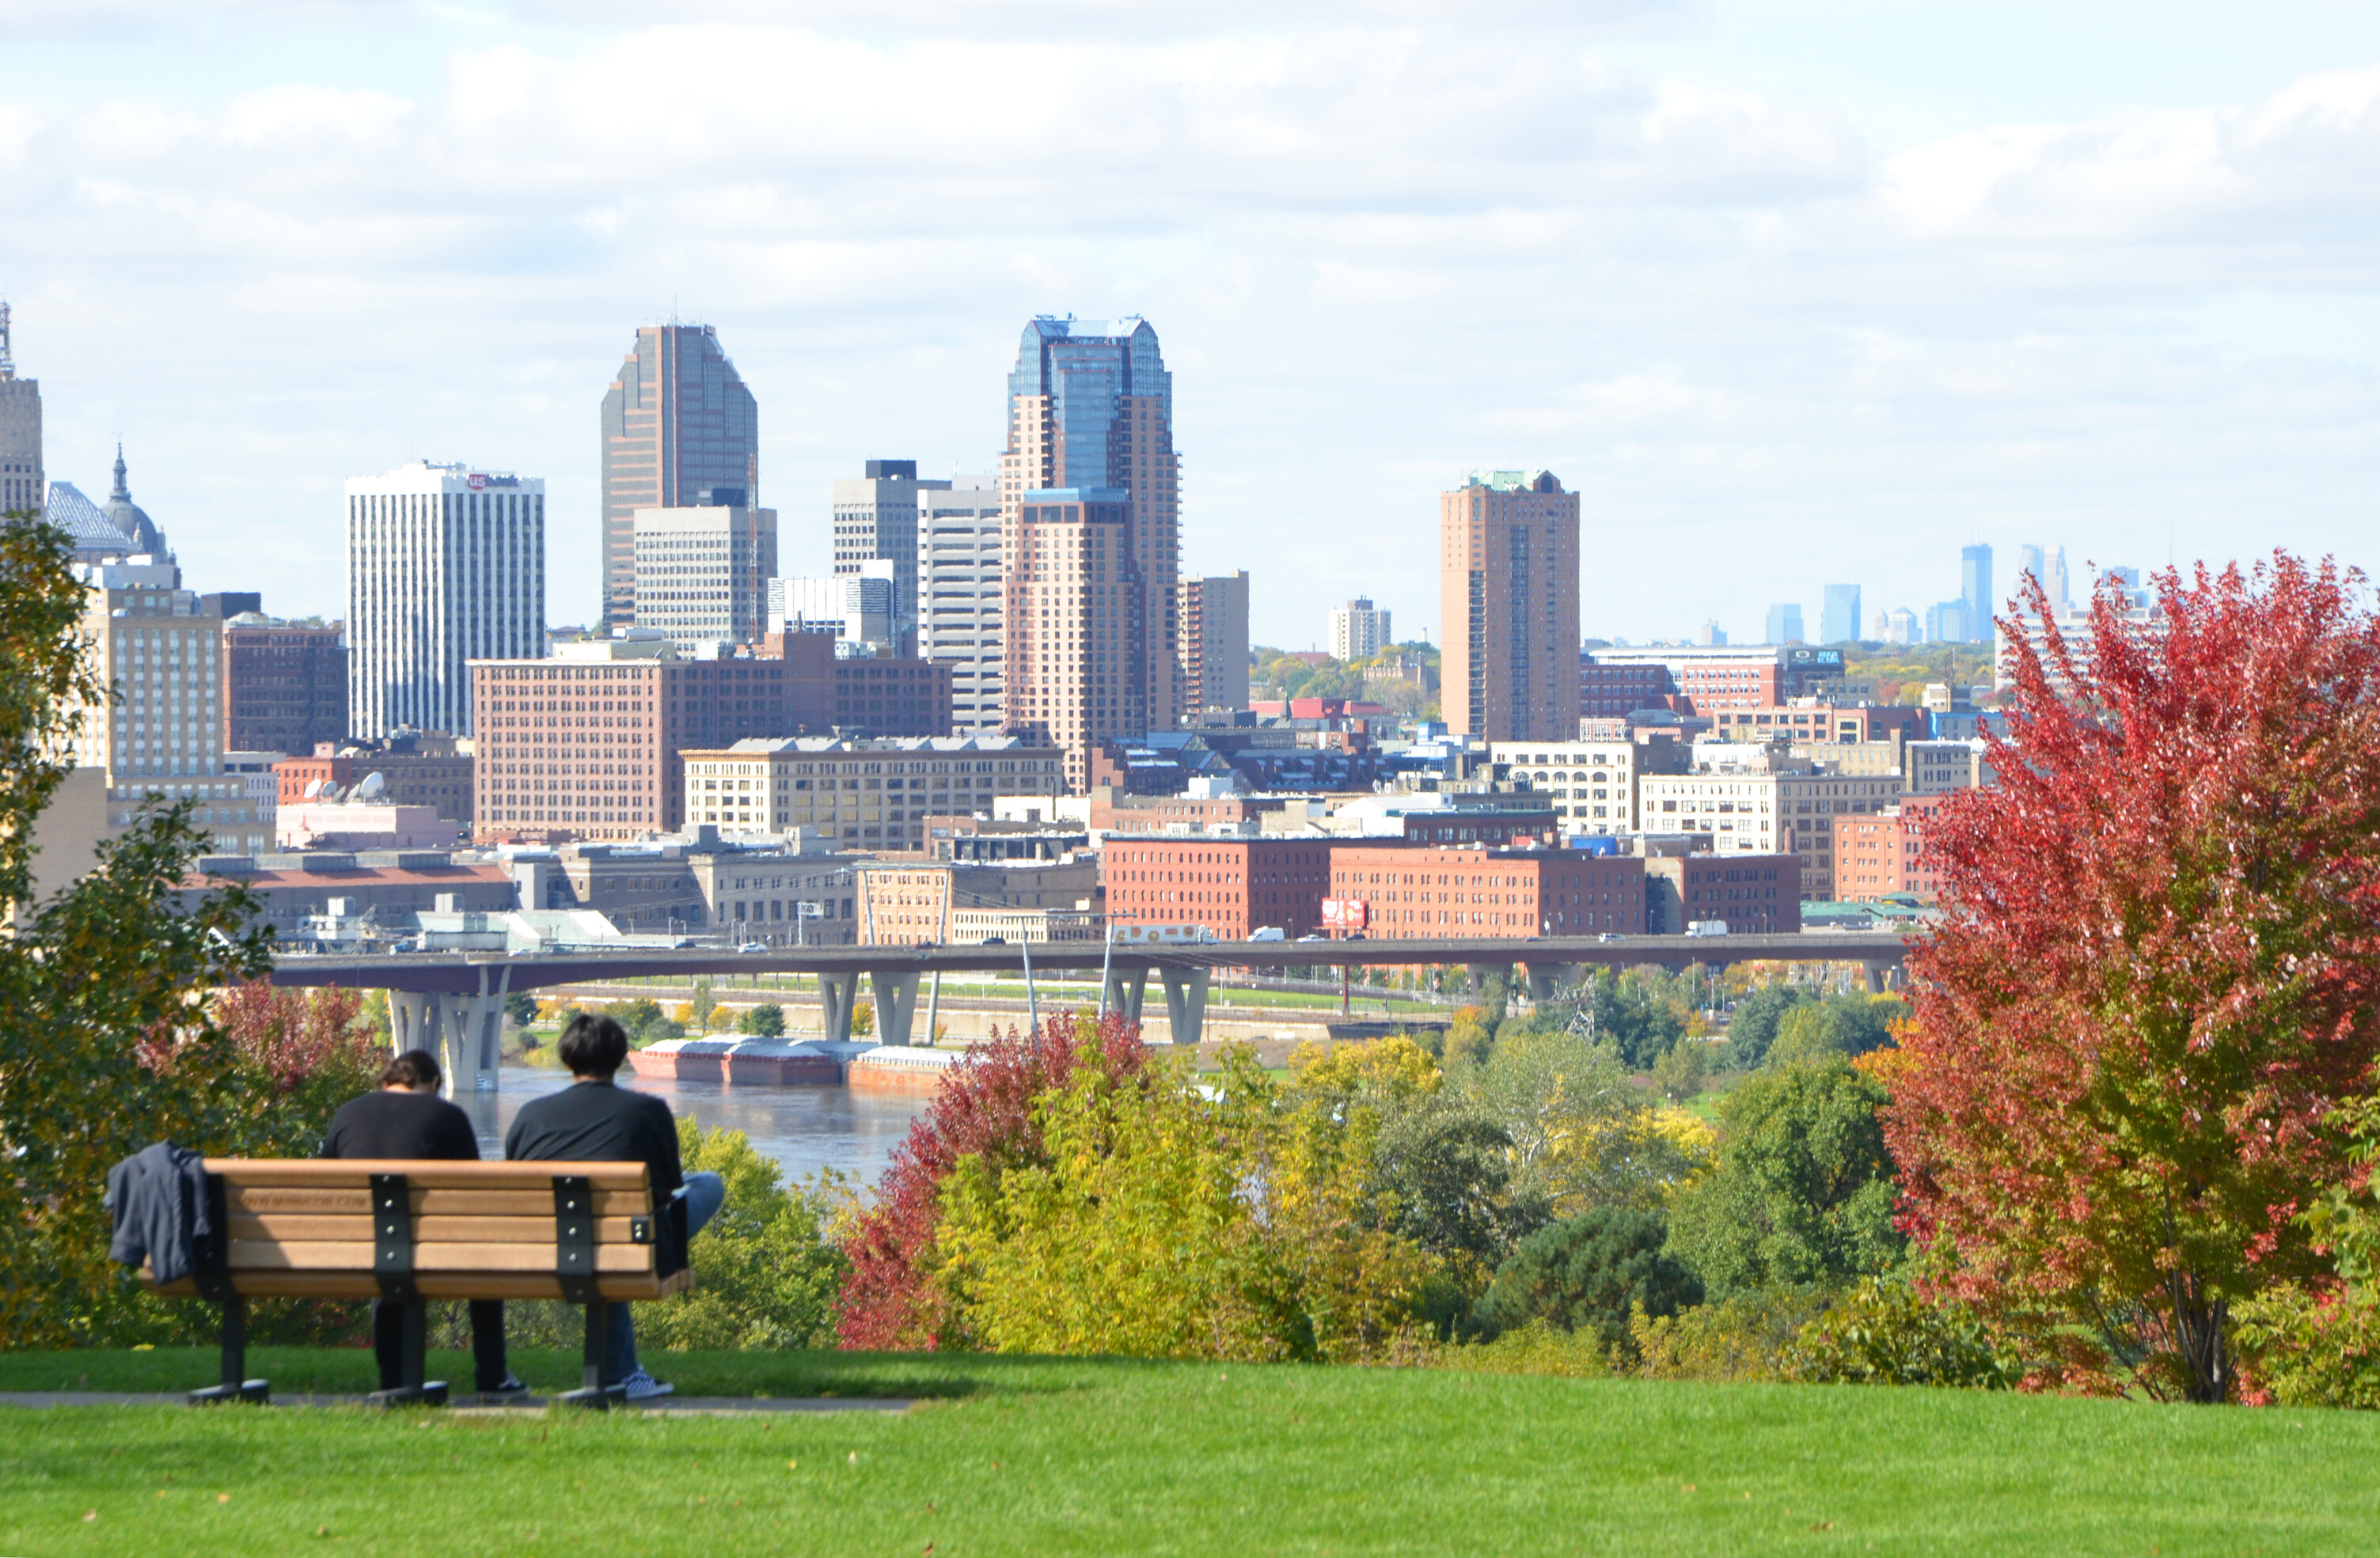
\includegraphics{images/3746.jpg}

The Greenhouse Gas Scenario Planning Tool uses the best available demographic assumptions for cities in the Metropolitan Region to forecast emissions in 2040.

Some common predictors of greenhouse gas emissions at the city scale include:

\begin{itemize}
\item
  \textbf{\emph{Population Density}} Minneapolis, the largest city in Minnesota, has a high population density. Higher density means more people live in a relatively small area compared to other regions' cities. Higher population densities are often associated with increased energy consumption, as residents need to use energy for daily activities and power local businesses. However, higher population density can also lead to more efficient use of resources and infrastructure, which can ultimately reduce the environmental impact of development in an area.
\item
  \textbf{\emph{Economic Activity}} According to the \href{https://mn.gov/deed/data/economic-analysis/compare/compare-metro/economy/gdp.jsp}{Minnesota Department of Employment and Economic Development}, the Twin Cities region ranks 8th in the country in terms of Gross Domestic Product (GDP) following the Denver region. Cities with higher levels of economic activity, such as manufacturing or transportation, tend to consume more energy due to the increased energy demand of these activities.
\item
  \textbf{\emph{Urban Planning}} The physical layout of a city can also affect energy consumption. For example, cities with more compact, walkable neighborhoods may have lower energy consumption due to the reduced need for transportation. The \href{https://go.minneapolismn.gov/}{Minneapolis Transportation Action Plan} was formally adopted by the Minneapolis City Council on December 2020. The plan discusses how in the past, streets have been designed primarily with car movement in mind, leading to wide roads and complex intersections that can be uncomfortable or difficult for pedestrians, bicyclists, and those with special mobility needs to navigate. The city has recognized these issues and has adopted policies such as the Climate Action Plan and the Complete Streets Policy to prioritize people over cars in street design and create more welcoming public spaces for all community members.
\item
  \textbf{\emph{Extreme Climate}} Minneapolis has a humid continental climate, which is characterized by hot summers and cold winters. The climate of a city can play a significant role in energy consumption. For example, more energy may be needed for heating in colder regions, while in hotter regions, more energy may be needed for air conditioning.
\item
  \textbf{\emph{Energy efficiency}} Finally, a city's energy consumption may be influenced by the efficiency of its energy use. For example, cities with more energy-efficient buildings and transportation systems may consume less energy overall. Since adopting the Climate Action Plan in 2013, Minneapolis has implemented several programs and policies to reduce energy use in buildings, including a commercial benchmarking ordinance, a green cost share program, and a clean energy partnership with its electric and natural gas utilities. The city has also established a green building program to encourage the construction of high-performing, energy-efficient buildings.
\end{itemize}

We obtained baseline 2018 values for population, households, and employment from the \href{https://www.census.gov/programs-surveys/acs}{US Census and American Community Survey} (ACS), a nationwide survey conducted by the United States Census Bureau to collect data on a variety of social, economic, and demographic characteristics of the American population. In cases when there are data gaps for city-level data, the Greenhouse Gas Scenario Planning Tool defaults to average county-level assumptions (\textbf{Table} \ref{tab:tab-demographic-assumptions}).

The Metropolitan Council, as part of its responsibilities, produces a forecast of population, households, and employment for all cities within its region using the REMI PI Model, a computer-based forecasting system that projects future trends based on economic, demographic, and social data. This forecast for year 2040 helps the Council plan for the future needs of the region, including infrastructure, housing, and other resources. The floor area assumptions are based on an extrapolation of recent historic trends in floor area growth using data from the \href{https://www.hennepin.us/residents/property/property-information-search}{County Assessor Parcel} dataset and the Zillow \href{https://www.zillow.com/research/ztrax/}{ZTRAX} dataset.

\textbf{Figure} \ref{fig:figure-demographics} shows the comparison of population and households for Minneapolis in 2018 with the 2040 forecast.

\label{tab:tab-demographic-assumptions}Demographics for Minneapolis

Variables

Minneapolis 2018

Hennepin Co.~2018

Minneapolis 2040

Households

182,719.00

NA

212,500.00

Population

428,483.00

NA

485,000.00

Jobs

333,471.00

NA

360,000.00

Commercial Jobs

256,713.00

511,466.00

292,134.00

Industrial Jobs

42,266.00

90,604.00

71,226.00

Number of Single Family Units

76,935.00

NA

76,494.00

Number of Multifamily Units

123,504.00

NA

145,653.00

Single Family Average Floor Area (ft2)

1,359.56

1,542.44

1,563.49

Multifamily Average Floor Area (ft2)

1,105.92

1,132.31

1,099.40

\hypertarget{building-energy}{%
\chapter{Building Energy}\label{building-energy}}

\includegraphics{../images//3090.jpg}

There are several strategies that can be employed to reduce emissions in the building energy sector, including improving efficiency, transitioning to low-carbon electricity sources, electrifying heating systems, adopting sustainable construction practices, and changing behaviors to use energy more efficiently.

\hypertarget{framework}{%
\section{Framework}\label{framework}}

The global energy consumption of buildings, both residential and commercial, has steadily increased and now accounts for between 20-40\% of energy consumption in developed countries (\protect\hyperlink{ref-perez-lombard_review_2008}{Pérez-Lombard, Ortiz, and Pout 2008}).

\textbf{What drives greenhouse gas emissions in the building sector?}

To make predictions about the future greenhouse gas emissions from the building energy sector in the city of r params\$ctu\_selection, we need to consider three important assumptions:

\begin{enumerate}
\def\labelenumi{\arabic{enumi})}
\item
  Residential energy consumption is proportional to the floor area of homes. In other words, larger homes consume more energy. Strategies aimed at reducing the floor area or increasing the energy efficiency per unit area of residential buildings have the potential to lower emissions. However, it's important to keep in mind that there are other factors that also contribute to residential energy consumption, such as the type of appliances and systems used, the number of occupants, and the home's location and climate.
\item
  Energy consumption in the non-residential sector is correlated with the number of jobs in the industrial and commercial sectors in a community. Strategies that reduce the energy intensity per worker have the potential to decrease greenhouse gas emissions by increasing energy efficiency. However, it's important to keep in mind that there are other factors that also contribute to non-residential energy consumption, such as the type of building, the usage pattern, and the location and climate.
\item
  The building sector is a major contributor to greenhouse gas emissions, primarily due to energy consumption. However, we have the opportunity to make a positive impact by reducing these emissions through decarbonizing our electricity grid and minimizing the carbon footprint of the natural gas used for heating, with strategies such as renewable natural gas.
\end{enumerate}

\textbf{Energy efficiency}

There are various energy-efficient building design standards available, such as Passive House standards, which consume less than 18 kilo BTUs per year, as well as new LEED performance-based energy efficiency standards. Minnesota's B3 Buildings Benchmarking project provides a long-term approach to tracking increases in the energy efficiency of existing and new buildings per square foot.

For instance, cities like Minneapolis, St.~Paul, St.~Louis Park, Edina, and Bloomington have encouraged energy-efficient buildings by adopting policies that require benchmarking for buildings. Building owners in Minneapolis can submit and view data online, and property managers and owners in Edina can view energy use for large buildings through an online map. In the vicinity of Bemidji, MN, the Waldsee BioHaus, a classroom and dormitory, holds the distinction of being the first building in North America certified by Germany's Passivhaus Institute.

\textbf{What is the status of the electricity grid?}

When it comes to reducing emissions in the building sector, the electricity grid, and the percent that it is supplied by renewable sources plays a major role.

Electricity in Minneapolis is served mostly by Xcel Energy. In their report \emph{Building a Carbon Free Future} in 2019, the utility states their goal to provide carbon-free electricity to all of its customers by 2050. The company aims to reduce carbon emissions by 80\% by 2030 as an interim goal.

New legislation signed by Governor Tim Walz sets a goal of having 100\% clean electricity in the state by 2040 (\href{https://mn.gov/commerce/news/?id=17-563384}{Governor Walz Signs Bill Moving Minnesota to 100 Percent Clean Energy by 2040}). However, there are many other factors and strategies that can be considered and implemented for efficiency, reduced demand, and reduced reliance on natural gas.

\hypertarget{residential-energy}{%
\section{Residential Energy}\label{residential-energy}}

The biggest share of residential energy use is typically for heating and cooling. In the United States, heating and air conditioning account for \href{https://www.eia.gov/energyexplained/use-of-energy/homes.php}{about half of the average home's energy use}. Therefore, for the residential sector, electricity and natural gas used tend to be closely correlated with the size of a building.

\textbf{Table} \ref{tab:tab-residential-energy} shows the basic assumptions about electricity and natural gas use for Minneapolis in the baseline year of 2018 and forecast year of 2040.

\label{tab:tab-residential-energy}Baseline Residential Energy Assumptions for Minneapolis

Variables

2018 (Baseline)

2040 (Busines-as-Usual)

Residential Electricity (MWh)

1,029,006

954,909

Residential Electricity Emissions (tonnes CO2e)

378,435

Residential Natural Gas (Therms)

120,984,119

140,340,271

Residential Natural Gas Emissions (tonnes CO2e)

643,172

Residential Electricity per Floor Area (KWh/ft2)

4.20961

3.36769

Residential Therms per Floor Area (therms/ft2)

0.494939

0.494939

Residential Electricity per Household (MWh/household)

5.63163

Residential Therms per Household (therms/household)

662.132

\hypertarget{strategies}{%
\subsection{Strategies}\label{strategies}}

Energy consumption depends on many factors including floor area, efficiency and insulation, grid composition, and of course the weather. We have calculated the impact of different strategies that alter each factor that is under human control.

Cities have a range of tools at their disposal to control the size of new single family homes and to encourage the construction of smaller, more efficient homes.

The City of Minneapolis can influence the factors around residential energy use in a variety of ways, including:

\begin{itemize}
\item
  \textbf{\emph{Design guidelines:}} Cities can adopt or develop design guidelines that specify the size and appearance of new single family homes. These guidelines can be used to encourage the construction of smaller or more efficient homes. There are several different energy efficiency building design standards, such as Passive House standards as well as LEED performance-based energy efficiency standards and others that could be used as guidelines for residential buildings.
\item
  \textbf{\emph{Zoning regulations:}} The City of Minneapolis has a range of residential zoning categories, including single-family, multifamily, and mixed-use zones, which are designed to accommodate different types of housing and land uses. The \emph{Minneapolis 2040 Comprehensive Plan} aimed to increase housing supply and address affordability and segregation issues by eliminating single-family zoning and allowing up to three units per property. A city could also use zoning regulations to specify the size of new single family homes. For example, the city might require that new single family homes have a minimum or maximum square footage, or that they be a certain percentage of the size of the lot on which they are built.
\item
  \textbf{\emph{Incentives:}} a city can offer incentives to encourage particular types of construction or renovation. For example, a city might offer reduced permit fees or other financial incentives to builders who construct homes that meet certain size requirements, or put forward funds for retrofitting existing homes for greater efficiency.
\item
  \textbf{\emph{Fees:}} Cities can impose impact fees on new construction in order to offset the costs of providing infrastructure and other services. Impact fees can be used to discourage the construction of larger homes by imposing higher fees on larger homes.
\end{itemize}

\hypertarget{increased-multifamily}{%
\subsubsection{Increased Multifamily}\label{increased-multifamily}}

Compact community development can reduce building energy use by increasing the proportion of multifamily homes in the housing stock. Multifamily homes have a smaller floor area than single-family homes, which can translate to energy use reductions.

The Metropolitan Council's Thrive MSP plan projects an increase in the percentage of multifamily housing by 2040. This is consistent with the Minneapolis 2040 plan move to eliminate single-family-only zoning areas.

\textbf{\emph{About this strategy}} Here, we model that \texttt{50\%} of all new single-family construction will become multifamily, with the multifamily homes having smaller square footage.

\label{tab:tab-increased-multifamily}New Single-Family Home Floor Area for Minneapolis

Variables

2018 Baseline

2040 Scenario

Number of Single Family Units

76,935.00

76,426.02

Number of Multifamily Units

123,504.00

145,653.00

Single Family Average Floor Area (ft2)

1,359.56

1,563.49

Multifamily Average Floor Area for the County (ft2)

1,132.31

1,125.64

\label{tab:fig03a1}New Single-Family Home Floor Area for Minneapolis

Variables

2018 Baseline

2040 Business-as-Usual

2040 Scenario

Residential Electricity (MWh)

1,029,006

954,909

954,876

Residential Electricity Emissions (kg CO2e)

582,829,127

540,860,391

540,841,819

Residential Natural Gas (Therms)

120,984,119

140,340,271

140,335,452

Residential Natural Gas Emissions (kg CO2e)

642,425,672

745,206,837

745,181,248

\includegraphics{_main_files/figure-latex/unnamed-chunk-42-1.pdf}

\textbf{Affordability co-benefit}: With electricity costs projected to nearly double by 2040, smaller floor area is likely to be more affordable for families in all types of housing. However, single-family floor areas in the Twin Cities are increasing. Therefore, the next section also demonstrates the effect of more affordable, smaller floor area, even in new single-family construction, going forward.

\hypertarget{reduce-average-single-family-floor-area-increase}{%
\subsubsection{Reduce Average Single-Family Floor Area Increase}\label{reduce-average-single-family-floor-area-increase}}

Over time, the single-family home average floor area has been increasing. The floor area of a home is directly correlated with energy use. If the availability of fossil fuel sources such as oil, natural gas, and coal is limited, energy prices may increase as demand outstrips supply. New single-family homeowners may respond to increased energy prices by choosing smaller living spaces in order to save on energy costs, driving market demand to decrease the average floor area of a new single-family home. Cities could also consider methods to influence the size of new single-family construction.

\textbf{\emph{About this strategy}} For this strategy, average single-family home size is modeled to be \texttt{5\%} larger in 2040 than in 2018 - as opposed to the business-as-usual prediction of \texttt{15\%}. We apply this impact to \texttt{50\%} of new single-family homes.

** LM: Do we want to combine these 2 tables?? **

\label{tab:tab-new-single-family-home-area}New Single-Family Home Floor Area for Minneapolis

Variables

2018 Baseline

2040 Scenario

Number of Single Family Units

76,935.00

76,426.02

Number of Multifamily Units

123,504.00

145,653.00

Single Family Average Floor Area (ft2)

1,359.56

1,563.49

Multifamily Average Floor Area for the County (ft2)

1,132.31

1,125.64

\label{tab:fig03a2}New Single-Family Home Floor Area for Minneapolis

Variables

2018 Baseline

2040 Business-as-Usual

2040 Scenario

Residential Electricity (MWh)

1,029,006

954,909

954,551

Residential Electricity Emissions (kg CO2e)

582,829,127

540,860,391

540,657,660

Residential Natural Gas (Therms)

120,984,119

140,340,271

140,287,667

Residential Natural Gas Emissions (kg CO2e)

642,425,672

745,206,837

744,927,511

\includegraphics{_main_files/figure-latex/unnamed-chunk-45-1.pdf}

\hypertarget{new-single-family-homes-energy-efficiency}{%
\subsubsection{New Single Family Homes Energy Efficiency}\label{new-single-family-homes-energy-efficiency}}

New construction can achieve much greater energy efficiency in comparison to existing buildings. There are many green building rating systems available for use, such as Green Communities, Energy Star, DOE Zero Energy Ready Homes, Passive House, LEED, or SB 2030. Cities could implement programs to encourage uptake of these standards.

The amount of energy savings that can be achieved through these guidelines and certifications will depend on the specific design and construction practices that are used, as well as the location and climate of the building.

The Greenhouse Gas Scenario Planning Tool uses \emph{LEED Gold} for residential buildings as an example of how building standard could reduce energy use and therefore carbon emissions.

\emph{LEED} (Leadership in Energy and Environmental Design) is a well-known green building rating system that is used to evaluate the sustainability of buildings. Buildings that meet \emph{LEED} standards are designed and constructed to be energy efficient and to use fewer natural resources. According to the \href{https://www.usgbc.org/leed/rating-systems/residential}{U.S. Green Building Council}, buildings that are designed to meet \emph{LEED} Gold standards typically achieve energy savings of around 25\% compared to conventional buildings.

\textbf{\emph{About this strategy}} We assumed \texttt{50\%} of new single-family homes to be LEED-Gold or equivalent with both electricity and gas energy use intensity reduced \texttt{64\%}.

\label{tab:tab-new-home-efficiency}New Home Efficiency Minneapolis 2040 Assumptions

Variables

2018 Baseline

2040 Scenario

Number of Single Family Units

76,935.00

76,494.00

Number of Multifamily Units

123,504.00

145,653.00

Single Family Average Floor Area (ft2)

1,359.56

1,563.49

Multifamily Average Floor Area for the County (ft2)

1,132.31

1,125.64

\label{tab:unnamed-chunk-47}New Home Efficiency Minneapolis 2040

Variables

2018 Baseline

2040 Business-as-Usual

2040 Scenario

Residential Electricity (MWh)

1,029,006

954,909

902,374

Residential Electricity Emissions (kg CO2e)

582,829,127

540,860,391

511,104,605

Residential Natural Gas (Therms)

120,984,119

140,340,271

132,619,359

Residential Natural Gas Emissions (kg CO2e)

642,425,672

745,206,837

704,208,798

\includegraphics{_main_files/figure-latex/unnamed-chunk-49-1.pdf}

\hypertarget{existing-homes-energy-efficiency}{%
\subsubsection{Existing Homes Energy Efficiency}\label{existing-homes-energy-efficiency}}

There are multiple ways in which a city, like Minneapolis, can promote the retrofit of existing homes to gain energy efficiency. Some examples include:

\begin{itemize}
\item
  \textbf{\emph{Develop education and outreach programs}} Cities can develop education and outreach programs to inform homeowners about the benefits of energy-efficient home retrofits and how to access available resources and incentives. According to the Center for Energy and Environment (CEEE) \href{https://www.mncee.org/energy-disclosure-impact-report-january-2020-through-june-2022}{the Energy Disclosure Program} in Minneapolis aims to increase consumer awareness of energy performance in single-family homes in order to encourage the adoption of energy efficiency improvements. The program has been in place since January 2020 and is a part of the city's Truth in Sale of Housing (TISH) pre-sale inspection process. It involves gathering data on key energy efficiency attributes such as insulation and heating equipment, and communicating the results to home sellers and buyers in an Energy Disclosure Report. The program is being implemented in partnership with the Center for Energy and Environment and CenterPoint Energy, and this report summarizes findings from the first 30 months of programming.
\item
  \textbf{\emph{Offer financial incentives}} Cities can offer financial incentives, such as rebates or low-interest loans, to encourage homeowners to invest in energy-efficient home retrofits. The City of Minneapolis, offers incentives and \href{https://www2.minneapolismn.gov/business-services/licenses-permits-inspections/construction-permits-certificates/construction-code-rules-enforcement/incentives-rebates/}{rebates for homeowners} for replacing less efficient equipment.
\end{itemize}

\begin{itemize}
\item
  \textbf{\emph{Implement energy audits}} Minneapolis residents might be eligible for program such as the Home Energy Squads which free visits by energy auditors to income qualifying households. Cities can offer energy audits to help homeowners identify areas where their homes are losing energy and recommend cost-effective retrofits.
\item
  \textbf{\emph{Partner with local organizations}} Cities can partner with local organizations, such as non-profits or utility companies, to offer resources and assistance to homeowners interested in energy-efficient retrofits.
\end{itemize}

\hypertarget{retrofit-80-of-homes}{%
\paragraph{Retrofit 80\% of Homes}\label{retrofit-80-of-homes}}

\textbf{\emph{About this strategy}} Cities can provide incentives to homeowners to retrofit their properties for energy efficiency. We assume \texttt{80\%} of existing homes with energy use intensity reduced by \texttt{33\%}.

\label{tab:tab-existing-home-efficiency}Existing Home Efficiency Minneapolis 2040

Variables

2018 Baseline

Number of Single Family Units

76,494.00

Number of Multifamily Units

145,653.00

Single Family Average Floor Area (ft2)

1,043.82

Multifamily Average Floor Area for the County (ft2)

822.20

\label{tab:unnamed-chunk-51}New Home Efficiency Minneapolis 2040

Variables

2018 Baseline

2040 Business-as-Usual

2040 Scenario

Residential Electricity (MWh)

1,029,006

954,909

672,196

Residential Electricity Emissions (kg CO2e)

582,829,127

540,860,391

380,731,673

Residential Natural Gas (Therms)

120,984,119

140,340,271

98,790,717

Residential Natural Gas Emissions (kg CO2e)

642,425,672

745,206,837

524,578,709

\includegraphics{_main_files/figure-latex/unnamed-chunk-53-1.pdf}

\hypertarget{retrofit-remaining-20-of-into-passive-homes}{%
\paragraph{Retrofit Remaining 20\% of into Passive Homes}\label{retrofit-remaining-20-of-into-passive-homes}}

\textbf{\emph{About this strategy}} Same as previous strategy, except now the remaining \texttt{20\%} of homes are retrofitted to high passive house standards, which results in \texttt{66\%} reduction in energy use intensity (ZeroEnergy Design, 2021).

\label{tab:tab-existing-home-efficiency2}Existing Home Efficiency Minneapolis 2040

Variables

2018 Baseline

Number of Single Family Units

76,494.00

Number of Multifamily Units

145,653.00

Single Family Average Floor Area (ft2)

940.78

Multifamily Average Floor Area for the County (ft2)

747.67

\label{tab:unnamed-chunk-55}New Home Efficiency Minneapolis 2040

Variables

2018 Baseline

2040 Business-as-Usual

2040 Scenario

Residential Electricity (MWh)

1,029,006

954,909

609,095

Residential Electricity Emissions (kg CO2e)

582,829,127

540,860,391

344,991,151

Residential Natural Gas (Therms)

120,984,119

140,340,271

89,516,911

Residential Natural Gas Emissions (kg CO2e)

642,425,672

745,206,837

475,334,798

\includegraphics{_main_files/figure-latex/unnamed-chunk-57-1.pdf}

\hypertarget{behavior-change-for-residential-energy-efficiency}{%
\subsubsection{Behavior Change for Residential Energy Efficiency}\label{behavior-change-for-residential-energy-efficiency}}

implementing efficient messaging, in-home energy displays, and smart meters can be an effective way to reduce household energy use, but the actual impact may depend on the specific circumstances of each city and the participation rate of households in these actions.

\textbf{\emph{About this strategy}} In this example we assume efficient messaging, in-home energy display, and smart meters together reduce household energy use by \texttt{11\%}, with \texttt{100\%} of homes changing behaviors due to these actions.

\label{tab:tab-behavior-change}Behavior Change Minneapolis 2040

Variables

2018 Baseline

2040 Scenario

Number of Single Family Units

76,935.00

76,494.00

Number of Multifamily Units

123,504.00

145,653.00

Single Family Average Floor Area (ft2)

1,359.56

1,391.51

Multifamily Average Floor Area for the County (ft2)

1,132.31

1,001.82

\label{tab:unnamed-chunk-59}Behavior Change Minneapolis 2040

Variables

2018 Baseline

2040 Business-as-Usual

2040 Scenario

Residential Electricity (MWh)

1,029,006

954,909

849,869

Residential Electricity Emissions (kg CO2e)

582,829,127

540,860,391

481,365,748

Residential Natural Gas (Therms)

120,984,119

140,340,271

124,902,841

Residential Natural Gas Emissions (kg CO2e)

642,425,672

745,206,837

663,234,085

\includegraphics{_main_files/figure-latex/unnamed-chunk-61-1.pdf}

\hypertarget{clean-residential-electricity}{%
\subsubsection{Clean Residential Electricity}\label{clean-residential-electricity}}

The electricity grid can become cleaner by increasing the use of renewable energy sources such as solar, wind, and hydroelectric power, which produce significantly fewer greenhouse gas emissions than fossil fuels.

Cities can support uptake of clean electricity by facilitating programs that fund or offer incentives for implementing renewable energy technologies. Residents and property owners can support renewable energy by installing these technologies, including solar panels and heat pumps.

\textbf{\emph{About this strategy}}: In this example, due to decarbonizing the grid at \texttt{80\%} the emission factor of electricity decreases from \texttt{568} kg2e/MWh (2018 Minnesota state level) to \texttt{113} kgCO2e/MWh.

\label{tab:tab-decarbonize-residential-energy}Decarbonize Residential Energy Use Minneapolis 2040

Variables

2018 Baseline

2040 Business-as-Usual

2040 Scenario

Residential Electricity (MWh)

1,029,006

954,909

954,909

Residential Electricity Emissions (kg CO2e)

582,829,127

540,860,391

108,172,078

Residential Natural Gas (Therms)

120,984,119

140,340,271

140,340,271

Residential Natural Gas Emissions (kg CO2e)

642,425,672

745,206,837

745,206,837

\includegraphics{_main_files/figure-latex/unnamed-chunk-63-1.pdf}

\hypertarget{electrification-of-residential-heating}{%
\subsubsection{Electrification of Residential Heating}\label{electrification-of-residential-heating}}

Alongside grid changes, switching to more efficient electric options for heating and hot water such as heat pumps and tank-less water heaters can significantly reduce emissions. Only around \texttt{14\%} of homes in MN have currently adopted these new technologies.

The scenario planning model utilizes efficiency of the heat pump derived from pilot tests in Minnesota, so the results are more realistic for our region. Results are preliminary as heat pump efficiency continues to increase.

\textbf{About this strategy} For this strategy, we model the assumption that by 2040 \texttt{59\%} of homes are using air-source heat pumps and electric water heaters, instead of using gas for heating.

\label{tab:tab-electrify-residential-heating}Electrify Residential Heating 2040

Variables

2018 Baseline

2040 Business-as-Usual

2040 Scenario

Residential Electricity (MWh)

1,029,006

954,909

3,756,281

Residential Electricity Emissions (kg CO2e)

582,829,127

540,860,391

2,127,557,626

Residential Natural Gas (Therms)

120,984,119

140,340,271

77,187,149

Residential Natural Gas Emissions (kg CO2e)

642,425,672

745,206,837

409,863,760

\hypertarget{renewable-natural-gas}{%
\subsubsection{Renewable Natural Gas}\label{renewable-natural-gas}}

This report projects that homes not using electricity for space and water heating will switch from natural gas to renewable natural gas.

\textbf{Renewable natural gas}, also known as biogas, consists largely of methane, which can be captured and processed at solid waste landfills and wastewater treatment plants.1 This comes with multiple benefits: it reduces methane emissions that would otherwise be released from landfills and wastewater treatment plants, and it can replace fossil fuel as an energy source. Food waste digestion facilities, which produce renewable natural gas from organic scraps, can also reduce the volume of waste sent to the landfill, which would help to meet the Minnesota Legislature's goal of recycling a greater portion of solid wastes in the Twin Cities metropolitan area.2

\textbf{\emph{About this strategy}} Our assumption is that cities can control (or at least influence)\ldots{}

** LM: Do we want to take this section out of the report for now? **

\hypertarget{non-residential-energy}{%
\section{Non-Residential Energy}\label{non-residential-energy}}

Non-residential energy use refers to the energy consumption of commercial and industrial buildings, including both electricity and natural gas. The baseline data for energy use was obtained from Xcel Energy. The forecast of ``business-as-usual'' energy use is estimated by considering the number of people who are expected to work in these buildings.

In addition to electricity and natural gas, non-residential energy use may also include other energy sources such as propane, fuel oil, and renewable energy sources, some of which are not captured in this methodology. Accurate estimates of non-residential energy use can help Minneapolis make informed decisions about energy efficiency and conservation efforts.

\textbf{Table} \ref{tab:tab-non-residential-energy} shows the baseline and forecast assumptions for non-residential electricity and natural gas use for Minneapolis.

\label{tab:tab-non-residential-energy}Non-Residential Energy for Minneapolis

Variables

2018

2040

Commercial Natural Gas (Therms)

74,323,233.92

84,578,278.54

Industrial Natural Gas (Therms)

90,265,300.08

152,113,667.33

Commercial Electricity (MWh)

1,580,539.69

1,798,620.96

Industrial Electricity (MWh)

1,254,092.31

2,113,376.69

Commercial Natural Gas per Worker (therms/worker)

289.52

289.52

Industrial Natural Gas per Worker (therms/worker)

2,135.65

2,135.65

Commercial Electricity per Worker (MWh/worker)

6.16

6.16

Industrial Electricity per Worker (MWh/worker)

29.67

29.67

As shown in \ref{tab:tab-non-residential-energy} for making estimate about the business-as-usual energy use of the City of Minneapolis, we assue that energy use intensity per worker for the commercial and industrial sectors remain constant.

\hypertarget{strategies-1}{%
\subsection{Strategies}\label{strategies-1}}

One of the most effective strategies for commercial and industrial buildings is to enhance their energy efficiency, which can be achieved through the adoption of new technologies. In Minnesota, there are several programs aimed at supporting non-residential consumers.

The \textbf{Conservation Improvement Program (CIP)} is a policy aimed at improving energy efficiency and conservation in households and businesses in Minnesota. Funded by ratepayers and administered by over 180 electric and natural gas utilities, with oversight from the Minnesota Department of Commerce's Division of Energy Resources, CIP promotes energy-efficient technologies and practices to residential, commercial, and industrial customers through various programs, such as energy audits, rebates on high-efficiency appliances, LED lighting, and air conditioning cycling programs.

The \textbf{Energy Conservation and Optimization Act of 2021 (ECO Act)} aims to strengthen the state's energy conservation programs, reduce greenhouse gas emissions, and create local jobs through energy efficiency projects in homes and businesses. The ECO Act expands the Conservation Improvement Program and makes energy efficiency improvements available to low-income households, public schools, and investor-owned utilities.

The \textbf{Minnesota SB2030} program focuses on reducing emissions in commercial, industrial, and institutional buildings. The program sets standards for energy efficiency and renewable energy for new and renovated buildings, based on the building's energy use per square foot. Over time, these standards will become more stringent, with the goal of reducing energy use and carbon dioxide emissions. The program also takes into account the impact of electric vehicle charging infrastructure on a building's energy use.

\hypertarget{retofit-existing-commercial-building}{%
\subsubsection{Retofit Existing Commercial Building}\label{retofit-existing-commercial-building}}

Retrofitting existing commercial and industrial buildings is key for reducing GHG emissions and mitigating the impacts of climate change. Retrofits can be accomplished through various measures such as improving insulation, upgrading heating and cooling systems, and replacing outdated lighting systems with energy-efficient alternatives.

According to \href{https://ecodistricts.org/information-exchange/commercial-energy-retrofits/}{Eco Districts} there are two types of energy retrofits for commercial buildings: conventional and deep. Conventional retrofits focus on isolated upgrades with a short payback time, such as lighting and HVAC systems, while deep retrofits take a whole-building approach to achieve greater energy efficiency by addressing multiple systems at once. One option for promoting commercial building energy retrofits is \href{https://minnpace.com/}{PACE} (property assessed clean energy) programs, which allow property owners to finance energy-efficiency and renewable-energy projects through a property tax assessment, secured by a senior lien on the property.

\textbf{\emph{About this strategy}} Our assumption is that cities can promote a reduction in energy use intensity (EUI) by the retrofit of existing commercial buildings. We assume that \texttt{80\%} of existing commercial buildings are certified as LEED Gold by 2040. LEED Gold is assumed to reduce energy use intensity (EUI) of an existing building by \texttt{25\%}.

\textbf{GHG Impact Calculation}

\[\text{new total } kgCO_2e_{2040}^{commercial} = x * jobs_{2018}^{commercial} * 0.25 * \left( \frac{MWh}{jobs_{2018}^{commercial}} * \frac{kgCO2e}{MWh_{2040}^{commercial}} + \frac{therms}{jobs_{2018}^{commercial}} * \frac{kgCO_2e}{therm_{2040}^{commercial}} \right)\]
\emph{Where:}

\begin{itemize}
\item
  \(x\text{, where } 0 \le x \le 1\): The percentage of existing commercial buildings are LEED Gold (defaulted to 80\%)
\item
  \(25%
  \): The assumed reduction in energy intensity from retrofits
\item
  \(jobs_{2018}^{commercial}\): The number of commercial workers in 2018 (from Minnesota Quarterly Census of Employment and Wages)
\item
  \(MWh/jobs_{2018}^{commercial}\): The commercial electricity use per worker in 2018
\item
  \(kgCO2e/MWh_{2040}^{commercial}\): The projected electricity emission factor in 2040
\item
  \(therms/jobs_{2018}^{commercial}\): The projected commercial gas use per worker in 2040
\item
  \(kgCO_2e/therm_{2040}^{commercial}\): The projected natural gas emission factor in 2040
\end{itemize}

\label{tab:fig03b1}Retrofit Commercial Buildings Minneapolis 2040

Variables

2018 Baseline

2040 Busines-As-Usual

2040 Scenario

Commercial Electricity (MWh)

1,580,540

1,798,621

1,166,405

Industrial Electricity (MWh)

1,254,092

2,113,377

2,113,377

Commercial Natural Gas (Therms)

187,242,460

213,077,985

138,181,001

Industrial Natural Gas (Therms)

26,082,037

43,953,039

43,953,039

Total Industrial Emissions (tonnes CO2e)

2,738,288,645

3,580,590,207

2,824,800,150

\includegraphics{_main_files/figure-latex/unnamed-chunk-66-1.pdf}

\hypertarget{smart-grid-electrification}{%
\subsubsection{Smart Grid Electrification}\label{smart-grid-electrification}}

Smart grid and technologies are projected to reduce industrial electricity use by 11\% .

Achieving a net-zero grid requires transitioning to a smart grid. The smart grid can not only manage the load but also reduce energy use by approximately 11\% as shown in PNNL's ``\href{https://www.osti.gov/biblio/971445}{The Smart Grid: An Estimation of the Energy and CO2 Benefits}.'' This reduction will be applied to all electricity consumers connected to the grid. In this and the next strategy, we have assumed that the 11\% reduction will apply to 100\% of electricity use for commercial buildings. It is important to note that all commercial and industrial energy use is calculated based on the number of employees, not on square footage.

\textbf{\emph{About this strategy}} Our assumption is that by adopting technologies such as smart grid, \texttt{100\%} of industrial buildings in the city can reduce their electricity use by \texttt{11\%}.

\textbf{GHG Impact Calculation}

\[ \text{new electricity } kgCO_2e_{2040}^{industrial} = x * \left(jobs^{industrial}_{2040} * \frac{MWh}{jobs^{industrial}_{2040}} * 11\% \right) * \frac{kgCO_2e}{MWh}\]
\emph{Where:}

\begin{itemize}
\tightlist
\item
  \(x\text{, where } 0 \le x \le 1\): The percentage of industries in the smart grid (assumed to be 100\%)
\item
  \(jobs^{industrial}_{2040}\): The projected number of industrial workers in 2040
\item
  \(MWh/jobs^{industrial}_{2040}\) = The projected industrial electricity use per worker in 2040
\item
  \(11%
  \) = The percentage reduction in energy use due to smart grid, fixed at 11\%
\item
  \(kgCO2e/MWh\) = The projected electricity emission factor in 2040
\end{itemize}

\label{tab:fig03b2}Smart Grid Efficiency Minneapolis 2040

Variables

2018 Baseline

2040 Busines-As-Usual

2040 Scenario

Commercial Electricity (MWh)

1,580,540

1,798,621

1,798,621

Industrial Electricity (MWh)

1,254,092

2,113,377

2,113,377

Commercial Natural Gas (Therms)

187,242,460

213,077,985

213,077,985

Industrial Natural Gas (Therms)

26,082,037

43,953,039

43,953,039

Total Industrial Emissions (tonnes CO2e)

2,738,288,645

3,580,590,207

1,364,834,737

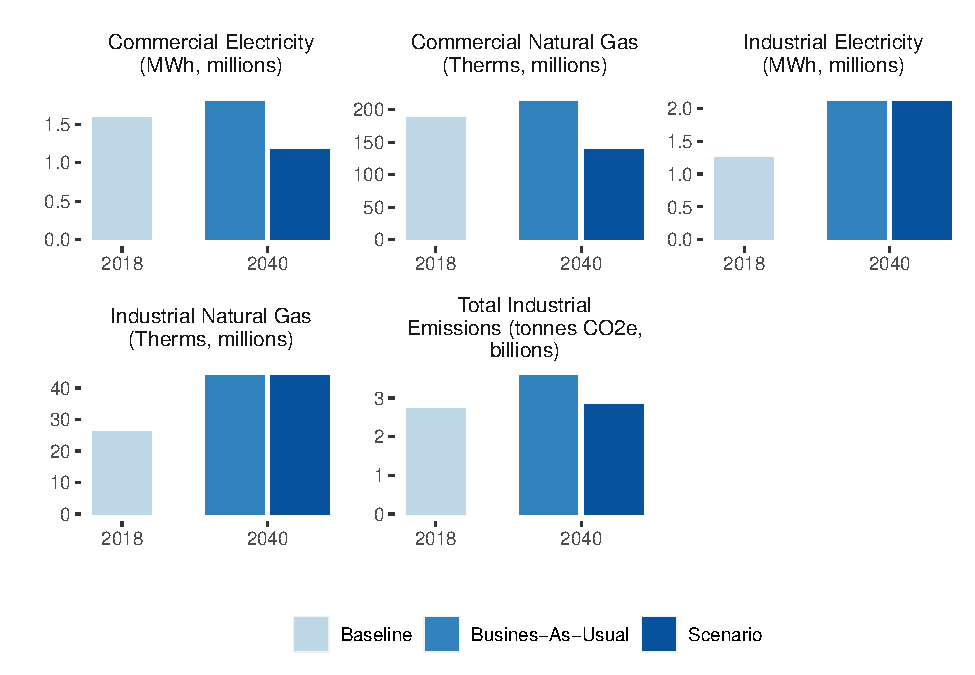
\includegraphics{_main_files/figure-latex/unnamed-chunk-67-1.pdf}

\hypertarget{renewable-natural-gas-1}{%
\subsubsection{Renewable Natural Gas}\label{renewable-natural-gas-1}}

We assume that renewable natural gas will substitute 31.7\% of all natural gas remaining in all the sectors. According to the American Biogas Council's estimate, Minnesota can produce 46.91 billion cu.ft renewable natural gas, which is 47 PJ. According to the Net-Zero America Report, 148 PJ will be needed in 2040 in the high efficiency and renewable scenario. Therefore, we assume that RNG can replace 31.7\% of remaining natural gas use at the state level. Estimates for New York State are available in Taboada et. al, 2021 (see references).

\textbf{\emph{About this strategy}} Our assumption is that cities can control (or at least influence)\ldots{}

\textbf{GHG Impact Calculation}

\[\text{new natural gas } kgCO_2e_{2040}^{nonresidential} = \left( jobs_{2040}^{commercial} * \frac{therms}{jobs_{2040}^{commercial}} + jobs_{2040}^{industrial}  * \frac{therms}{jobs_{2040}^{industrial}} \right) * x * \frac{kgCO_2e}{therms_{2040}}\]

\emph{Where:}

\begin{itemize}
\tightlist
\item
  \(x\text{, where } 0 \le x \le 1\) = The percentage of natural gas replaced by renewable natural gas (utility level), assumed to be \texttt{31.7\%}
\item
  \(jobs_{2040}^{commercial}\): The projected number of commercial workers in 2040
\item
  \(jobs_{2040}^{industrial}\): The projected number of industrial workers in 2040
\item
  \(therms/jobs_{2040}^{commercial}\): The projected commercial gas use per worker in 2040
\item
  \(therms/jobs_{2040}^{industrial}\): The projected industrial gas use per worker in 2040
\item
  \(kgCO_2e/therms_{2040}\): The projected emissions factor of natural gas in 2040
\end{itemize}

\label{tab:fig03b3}Retrofit Commercial Buildings Minneapolis 2040

Variables

2018 Baseline

2040 Busines-As-Usual

2040 Scenario

Commercial Electricity (MWh)

1,580,540

1,798,621

1,798,621

Industrial Electricity (MWh)

1,254,092

2,113,377

2,113,377

Commercial Natural Gas (Therms)

187,242,460

213,077,985

213,077,985

Industrial Natural Gas (Therms)

26,082,037

43,953,039

43,953,039

Total Industrial Emissions (tonnes CO2e)

2,738,288,645

3,580,590,207

1,364,834,737

\includegraphics{_main_files/figure-latex/unnamed-chunk-69-1.pdf}

\hypertarget{decarbonize-the-electricity-grid}{%
\subsubsection{Decarbonize the Electricity Grid}\label{decarbonize-the-electricity-grid}}

This strategy demonstrates the impact of grid decarbonization.

\textbf{\emph{About this strategy}} Our assumption is that cities can control (or at least influence)\ldots{}

\textbf{GHG Impact Calculation}

\[\text{new electricity }kgCO2e_{2040}^{nonresidential} = (jobs_{2040}^{commercial} * MWh_{2040}^{commercial} + jobs_{2040}^{industrial} * MWh_{2040}^{industrial}) * \left(\frac{kgCO_2e/MWh_{2040}}{1000}\right) * x\]
\emph{Where:}

\begin{itemize}
\tightlist
\item
  \(x\text{, where } 0 \le x \le 1\): = The percentage reduction in grid emission factor from 2018 (assumed to be 80\%)
\item
  \(jobs_{2040}^{commercial}\): The projected number of commercial jobs in 2040
\item
  \(MWh/jobs_{2040}^{commercial}\): The projected commercial electricity use per worker in 2040
\item
  \(jobs_{2040}^{industrial}\): The projected number of industrial jobs in 2040
\item
  \(MWh/jobs_{2040}^{industrial}\): The projected number industrial electricity use per worker in 2040
\item
  \(kgCO_2e/MWh_{2040}\): The projected electricity emission factor in 2040
\end{itemize}

Note: The values are multiplied by 1000 in the original formula to retain the units in kilowatt hours.

\label{tab:fig03b4}Decarbonise Grid Minneapolis 2040

Variables

2018 Baseline

2040 Busines-As-Usual

2040 Scenario

Commercial Electricity (MWh)

1,580,540

1,798,621

1,798,621

Industrial Electricity (MWh)

1,254,092

2,113,377

2,113,377

Commercial Natural Gas (Therms)

187,242,460

213,077,985

213,077,985

Industrial Natural Gas (Therms)

26,082,037

43,953,039

43,953,039

Total Industrial Emissions (tonnes CO2e)

2,738,288,645

3,580,590,207

1,364,834,737

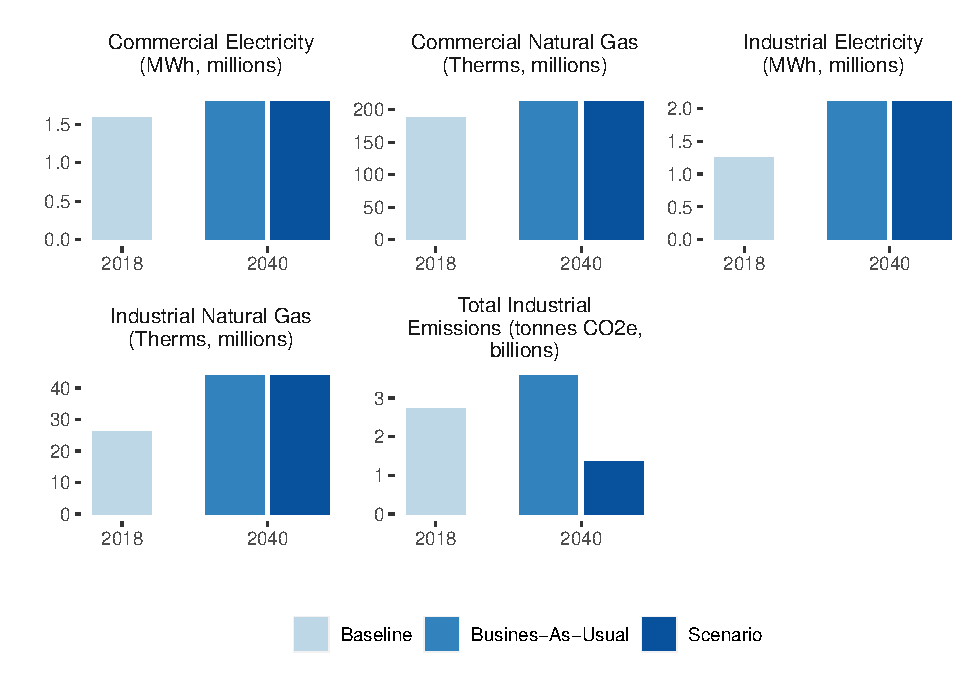
\includegraphics{_main_files/figure-latex/unnamed-chunk-70-1.pdf}

\hypertarget{transportation}{%
\chapter{Transportation}\label{transportation}}

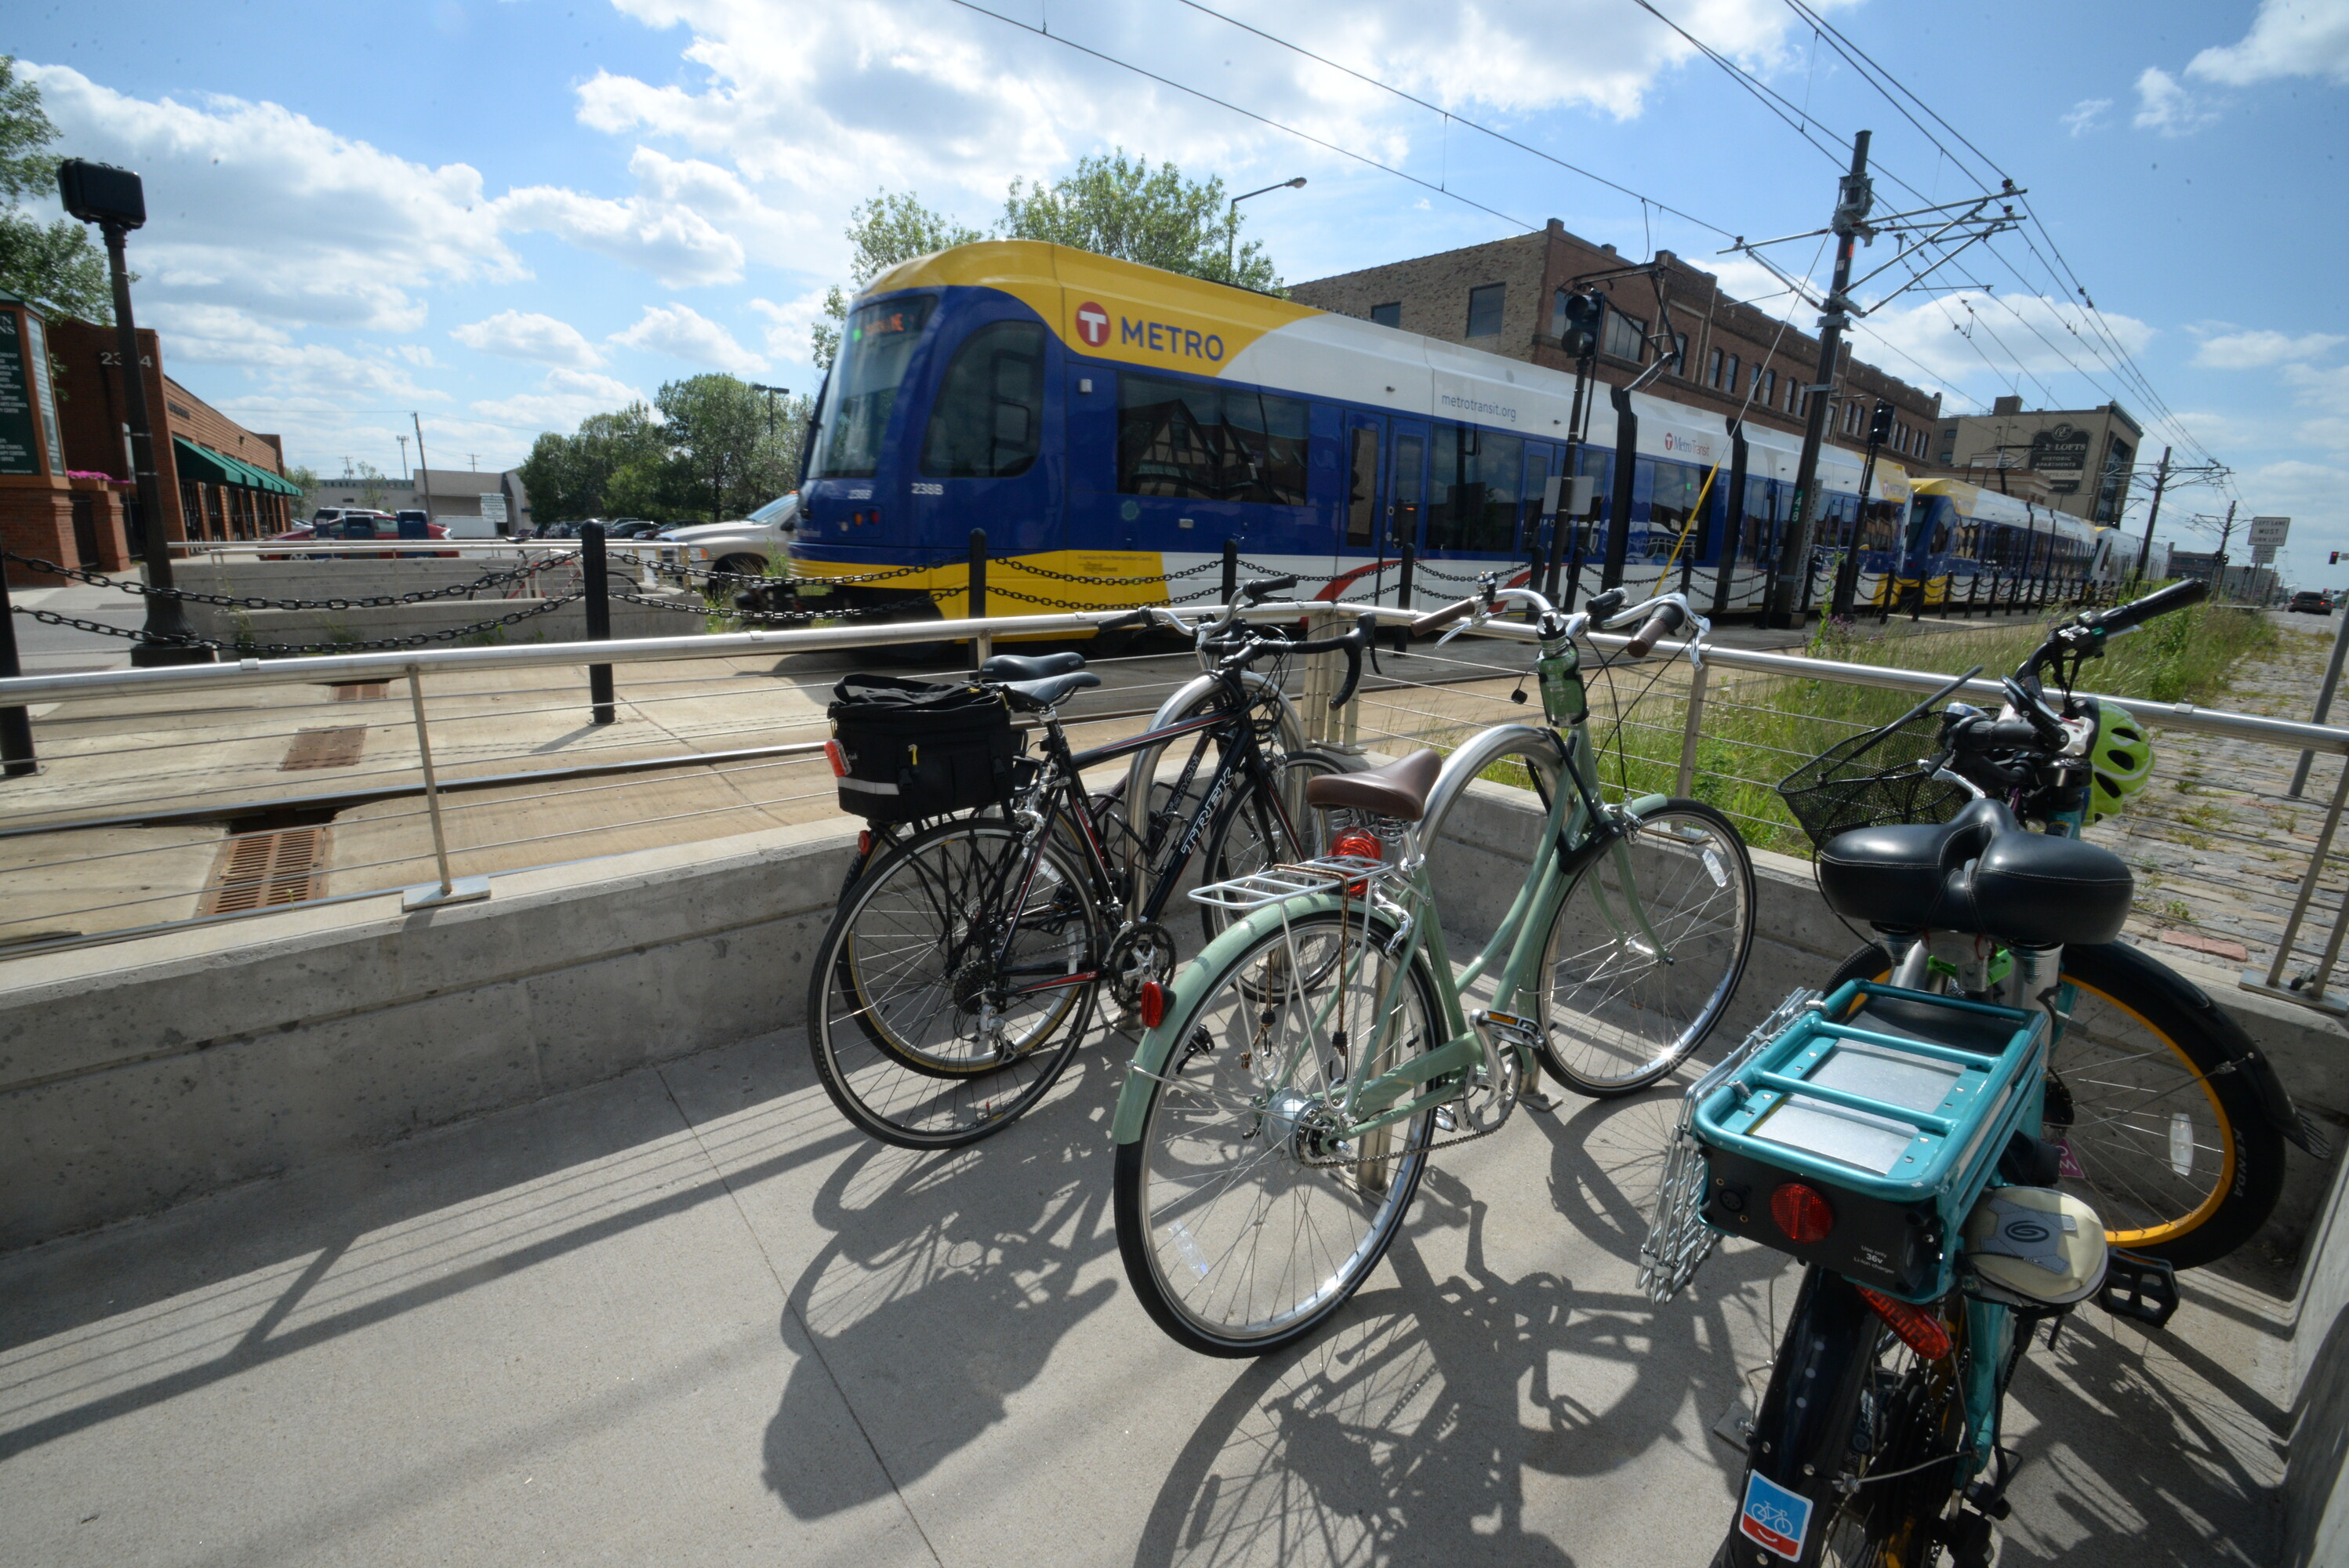
\includegraphics{images//2724.jpg}

The Metropolitan Council Transportation Policy Plan notes that the rapid expansion of the region's developed area in an ``auto-centric'' manner has resulted in longer average trips and the diminished attractiveness of non-auto modes as modes of regional travel. The issue of longer and more frequent automobile trips contributes to the challenge of reducing greenhouse gas emissions.

Instead, when land use and transportation systems are designed to work together, they can create more efficient and sustainable communities. For example, compact, walkable communities with a mix of land uses can reduce the need for driving and improve the transportation system's efficiency.

\hypertarget{framework-1}{%
\section{Framework}\label{framework-1}}

Ramaswami, Fang, and Tabory (\protect\hyperlink{ref-ramaswamiReviewIntegratedUrban2020}{Ramaswami, Fang, and Tabory 2020}) provide a framework for urban planning tools for greenhouse gas (GHG) mitigation as shown in as four key levers of action based on the framework developed in previous work by the UN International Resource Panel (\protect\hyperlink{ref-swillingWeightCitiesResource2018}{Swilling et al. 2018}).

It is found that transit and car-sharing become cost-effective beyond a density of 35 dwelling units per acre (\protect\hyperlink{ref-santasieriPlanningTransitSupportiveDevelopment2014}{Santasieri 2014}) and 5-10 dwelling units per acre (\protect\hyperlink{ref-millard-ballAutonomousVehicleParking2019}{Millard-Ball 2019}), respectively.

\hypertarget{transportation-baseline-and-data}{%
\section{Transportation Baseline and Data}\label{transportation-baseline-and-data}}

The Council is in the process of verifying data sources for all inputs and values.

The inputs for the transportation sector baseline and forecast are:

\begin{itemize}
\tightlist
\item
  \textbf{Passenger Miles Traveled} (PMT) forecasts from Metropolitan Council \href{https://metrocouncil.org/Transportation/Performance/Travel-Forecasting.aspx}{Regional Transportation Demand Model (RTDM)}.
\item
  \textbf{The Transportation Demand Model} A transportation demand model is a tool that is used to predict how people and goods will move within a transportation system. It can be used to forecast the demand for different modes of transportation, such as cars, buses, trains, and planes, and to evaluate the impacts of different transportation policies and investments.
\item
  \textbf{Average vehicle occupancy by mode}
\item
  \textbf{MA3T stock turnover and adoption forecasts by ``powertrain''}: SI (spark ignition gasoline) vehicles, CI (combustion emissions diesel) vehicles, hybrid-electric vehicles (HEVs), plug-in hybrid-electric vehicles (PHEV), and battery-electric. \href{https://teem.ornl.gov/ma3t.shtml}{MA3T} stands for Market Acceptance of Advanced Automotive Technologies (MA3T) and it allows to simulate the diverse purchasing behaviors among individuals in the market place.
\end{itemize}

\hypertarget{annual-energy-outlook-aeo}{%
\subsection{Annual Energy Outlook (AEO)}\label{annual-energy-outlook-aeo}}

In addition to the inclusion of the strategies outlined, alternative future scenarios are adopted from the EIA Annual Energy Outlook.

The inclusion of these scenarios allows the user to easily consider uncertainty in global financial and energy markets. The AEO scenarios are included as variations in fuel economy and VMT by mode. The following AEO scenarios are included in the tool (\protect\hyperlink{ref-eiaAnnualEnergyOutlook2021}{{``Annual {Energy Outlook}''} 2021}).

\begin{enumerate}
\def\labelenumi{\arabic{enumi}.}
\tightlist
\item
  \textbf{High oil price} the price of Brent crude oil, in 2020 dollars, reaches \$173 per barrel by 2050 compared with \$95 per barrel in the reference case.\\
\item
  \textbf{Low oil price} the price of Brent crude oil, in 2020 dollars, drops to \$48 per barrel by 2050 compared with \$95 per barrel in the reference case.\\
\item
  \textbf{High economic growth} U.S. GDP grows by 2.6\% per year compared with 2.1\% in the reference case.\\
\item
  \textbf{Low economic growth} U.S. GDP grows by 1.6\% per year compared with 2.1\% in the reference case.
\end{enumerate}

The AEO analysis includes two additional scenarios representing high and low renewable cost cases, respectively. We do not consider these cases as we rely on Xcel Energy electricity grid forecasts in the tool and variation in renewable prices would affect these assumptions.

\hypertarget{passenger}{%
\subsection{Passenger}\label{passenger}}

The Twin Cities region relies heavily on private cars for transportation, with options including gasoline, diesel, hybrid electric-gasoline, plug-in hybrid electric-gasoline, and battery electric vehicles.

The region's transportation carbon emissions are calculated based on data on vehicle usage, average vehicle occupancy, and person miles traveled by mode. Public transit options include urban and interurban buses and rails, with the option to switch to electric power in the future. Public transit mode shares are estimated using definitions from the \href{https://metrocouncil.org/Transportation/Performance/Travel-Behavior-Inventory.aspx}{2019 Travel Behavior Inventory (TBI)}, but there are no estimates of transit vehicle turnover to the 2050 forecast year.

The dominant mode of passenger transportation in MSP is the private car (i.e., passenger light-duty vehicle). Powertrain types included in the tool for this mode are gasoline, diesel, hybrid electric-gasoline (HEV), plug-in hybrid electric-gasoline (PHEV), and battery electric (BEV).

Public transit modes are categorized as urban bus, bus rapid transit (BRT), urban rail (LRT), and interurban rail (Northstar commuter rail). Bus modes have fuel options of biodiesel, hybrid electric-biodiesel, and battery electric. The LRT is already run by electricity and it is assumed that use of this technology will continue. The Northstar commuter rail currently uses biodiesel as an energy feedstock, but the option is available in the tool to switch it to an electric powertrain by 2050.

In the case of PHEV, there is a need to consider the fraction of VMT driven in electric and gasoline modes. It is assumed that the average travel distance in electric mode for a PHEV is 30 miles (\protect\hyperlink{ref-lovedayTopPlugInHybrid2019}{Loveday 2019}) and that households only recharge vehicles at night. Using these assumptions, the fraction of time operating in gasoline mode can be estimated based on 2019 TBI data for household vehicle usage for each CTU.

The regional model provides PMT totals for auto, transit, bike, and walk modes. PMT by mode is allocated to CTU using the standard 100-50-50 method given in the GHG Protocol for Cities (\protect\hyperlink{ref-theworldresourcesinstituteWRIAnnualReport2012}{The World Resources Institute 2012}). That is, 100\% of PMT for trips that start and end in the same CTU is allocated to that CTU. Otherwise, 50\% of PMT is allocated to each of the trip start CTU and trip end CTUs. A factor of 340 is used to convert daily PMT into annual PMT based on the recommendation of the Carbon Free Boston study (\protect\hyperlink{ref-porterCarbonFreeBoston2019}{Porter et al. 2019}).

\hypertarget{freight}{%
\subsection{Freight}\label{freight}}

The Twin Cities region is a critical transportation hub for the upper Midwest, serving as a distribution center for Minnesota, Wisconsin, North and South Dakota, and eastern Montana. The region is served by five modes of freight transportation: trucks, railroads, barges, air freight, and pipelines. These modes play a crucial role in supporting the region's economic competitiveness and quality of life by allowing residents to access the goods and materials they need and enabling businesses to distribute their products.

The region's freight transportation system is facing challenges, including congestion, lack of capacity, and infrastructure deficiencies, which need to be addressed to ensure the system's continued effectiveness. The Metropolitan Council works closely with the Minnesota Department of Transportation and other partners to ensure that the regional freight system supports a thriving and sustainable economy. Many freight-related improvements are the responsibility of private owners and operators of transportation modes and freight terminal facilities, although public investments in infrastructure also play a role.

\hypertarget{transportation-baseline-and-forecast}{%
\section{Transportation Baseline and Forecast}\label{transportation-baseline-and-forecast}}

\label{tab:tab-passenger-miles-traveled}Passenger Miles Traveled by Mode Minneapolis

Mode

2018

2040

Passenger light duty vehicle

3,879,556

3,669,647

Active transportation (walk and bike)

316,757

347,165

Urban bus (standard, non-BRT bus)

220,289

241,437

Bus rapid transit

5,126

5,618

Urban rail

78,635

86,183

Intercity rail

12,707

13,927

Walk

105,340

133,347

Bike

67,247

71,290

School bus

37,683

53,755

\label{tab:tab-freight-miles-traveled-forecast}Freight Miles Traveled by Mode - Minneapolis

Mode

2018

2040

Combined unit truck

684,122.58

937,773.0

Single unit truck

228,815.33

313,652.6

Freight rail

1,876,341.80

1,996,576.3

Multi-modal freight (combination of truck and rail)

441,925.81

655,486.4

Air freight

7,867.95

20,451.3

Water freight

0.00

0.0

Embodied emissions are a significant but often overlooked aspect of reducing carbon emissions in transportation from manufacturing and maintaining vehicles and infrastructure. Different vehicles and modes of transportation have different levels of embodied emissions. The GHG Tool in this study estimates embodied emissions for various types of passenger vehicles, public transit, and school buses based on an analysis by Chester and Horvath ((\protect\hyperlink{ref-Chester_Horvath_2009}{Chester and Horvath 2009})) and other sources. The tool considers the emissions resulting from manufacturing, maintenance, tire production, and other factors over the vehicle's lifetime. It does not currently estimate embodied emissions for freight vehicles as data on their stocks and sales is not available for the study area.

\hypertarget{interventionsstrategies}{%
\section{Interventions/Strategies}\label{interventionsstrategies}}

The transportation module uses passenger miles traveled as a proxy for emissions. Miles traveled are calculated for each travel mode and then converted into emissions.

\hypertarget{land-use}{%
\subsection{Land Use}\label{land-use}}

Transportation and land use policies are reliant on each other. Segregated and low-density land use patterns lead to a reliance on automobiles, increased vehicle miles traveled, and decreased efficacy of shared travel. However, altering land use policy is complex and only sometimes leads to changes in land use, as construction takes time to catch up with zoning. The scenario planning model uses the ``five D's'' (population and employment density, diversity of land uses, street design, distance to transit, and destination accessibility) as the land use factors that affect transportation.

The Metropolitan Council Transportation Policy Plan discusses the need for communities to consider the connections between land use and transportation as the region changes in the coming years. The plan mentions that it is not feasible to expand the highway system in a sustainable manner and that there is increased private investment in already developed parts of the region along transit lines. The Transportation Policy Plan also mentions that higher-density development and redevelopment occur in already-developed areas. That new growth is happening in suburban edge and emerging suburban edge communities, which stresses the regional highway system. The plan suggests that planners incorporate multimodal travel options, such as transit, walking, and biking, into land use and design to address issues like congestion, climate change, equity, and livability.

\textbf{\emph{About this strategy}} Increasing density decreases travel distances and encourages transit, cycling, and walking. We estimate a \texttt{0.4\%} decrease in auto VMT for a \texttt{10\%} increase in population density by 2040, a \texttt{7\%} increase in walking/cycling VMT for a \texttt{10\%} increase in population density by 2040, and a \texttt{7\%} increase in transit VMT for a \texttt{10\%} increase in population density by 2040.

\begin{longtable}{lrr}
\toprule
Land Use Adjustment & Multiplier relative to BAU & Effect on miles traveled by 2050 \\ 
\midrule
\multicolumn{3}{l}{Drive} \\ 
\midrule
Population density & +10\% & -4\% \\ 
Employment density & +10\% & +0\% \\ 
Land use diversity & +10\% & -9\% \\ 
Intersection design & +10\% & -12\% \\ 
Job accessability by transit & +10\% & -20\% \\ 
Distance to transit & -10\% & -5\% \\ 
\midrule
\multicolumn{3}{l}{Walk} \\ 
\midrule
Population density & +10\% & +7\% \\ 
Employment density & +10\% & +4\% \\ 
Land use diversity & +10\% & +15\% \\ 
Intersection design & +10\% & -6\% \\ 
Job accessability by transit & +10\% & -6\% \\ 
Distance to transit & -10\% & +15\% \\ 
\midrule
\multicolumn{3}{l}{Transit} \\ 
\midrule
Population density & +10\% & +7\% \\ 
Employment density & +10\% & +1\% \\ 
Land use diversity & +10\% & +12\% \\ 
Intersection design & +10\% & +29\% \\ 
Job accessability by transit & +10\% & +12.8\% \\ 
Distance to transit & -10\% & +29\% \\ 
\bottomrule
\end{longtable}

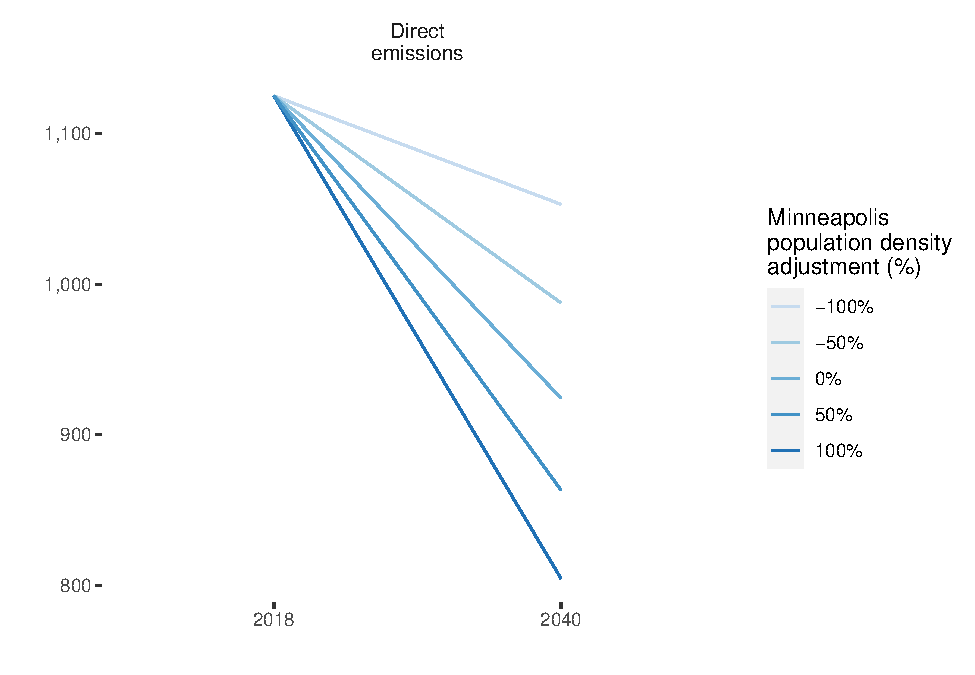
\includegraphics{_main_files/figure-latex/fig-landuse-1.pdf}

\label{tab:tab-land-use-scenario}Emissions in tonnes CO2e - 50\% Increase in Population Density Minneapolis

Mode

2018 Baseline

2040 Business-as-Usual

2040 Scenario

Bike

0.00

0.00

0.00

School bus

1.01

1.33

1.33

Urban bus (standard, non-BRT bus)

50.70

51.72

63.86

Passenger light duty vehicle

1,069.93

883.89

792.31

Intercity rail

0.17

0.18

0.22

Urban rail

3.78

4.49

5.54

Walk

0.00

0.00

0.00

\hypertarget{vehicle-electrification-1}{%
\subsection{Vehicle Electrification}\label{vehicle-electrification-1}}

The Greenhouse Gas Scenario Planning Tool aims to assess the potential impact of electric vehicles on greenhouse gas emissions in the Twin Cities metropolitan region.

The Tool uses data from the Market Acceptance of Advanced Automotive Technologies model to forecast electric vehicle market penetration in the region, and considers the GHG intensity of the region's electricity grid in calculating the GHG impact of electric vehicles.

The Tool also accounts for the fact that plug-in hybrid electric vehicles may operate in both electric and gasoline modes, and estimates the fraction of time that these vehicles operate in each mode based on the average distance that they can travel on electric power and data on household vehicle usage. The tool aims to provide insight into the potential for electric vehicles to reduce GHG emissions in the region and inform policy decisions related to electric vehicle adoption.

\begin{figure}

{\centering 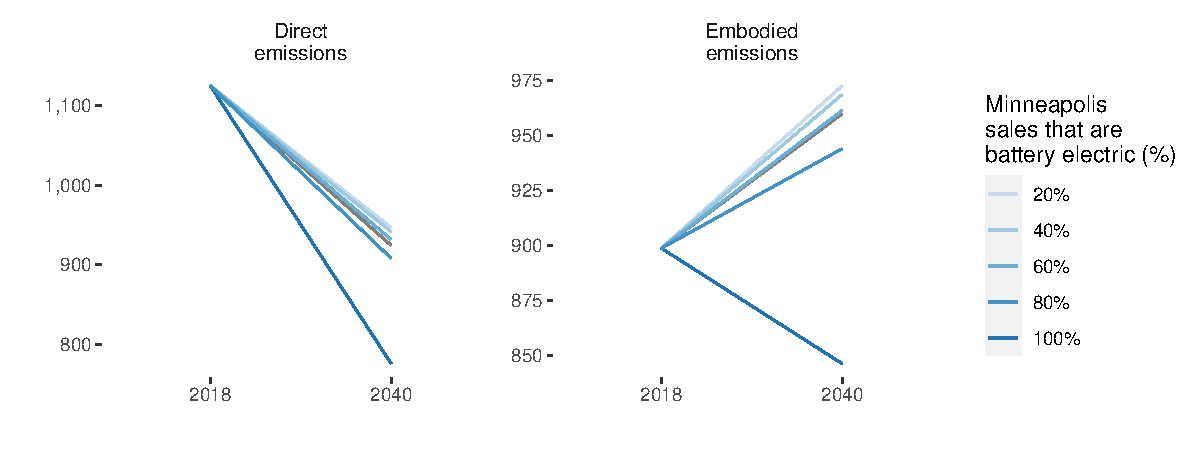
\includegraphics{_main_files/figure-latex/fig-bev-1} 

}

\caption{Comparing the direct and embodied greenhouse gas emissions between years 2018 and 2040 for different percentages of vehicles sales which are battery electric.}\label{fig:fig-bev}
\end{figure}

\label{tab:tab-bev-comp2}Emissions in tonnes CO2e - 60\% vehicle sales battery electric Minneapolis

Mode

2018 Baseline

2040 Business-as-Usual

2040 Scenario

Bike

0.00

0.00

0.00

School bus

1.01

1.33

1.33

Urban bus (standard, non-BRT bus)

50.70

51.72

51.72

Passenger light duty vehicle

1,069.93

883.89

873.82

Intercity rail

0.17

0.18

0.18

Urban rail

3.78

4.49

4.49

Walk

0.00

0.00

0.00

\hypertarget{public-transit}{%
\subsection{Public Transit}\label{public-transit}}

According to the \href{https://go.minneapolismn.gov/}{Minneapolis Transportation Action Plan (TAP)}, transit is essential for the city's multimodal transportation system. Transit contributes to economic competitiveness by attracting businesses, private investment, and top talent. Over 30,000 (16.5\%) households in the city do not have access to or choose not to own a personal car, with the highest concentration of car-free individuals living in neighborhoods around downtown Minneapolis. The TAP aims to improve the coverage, speed, and reliability of transit service through a partnership with the Metropolitan Council and by defining clear priorities, goals, and actions for the city. The goal is to increase the number of transit trips from 13\% in 2019 to 25\% by 2030. Transit must be convenient, reliable, and frequent and effectively reduce trips made by single-occupancy vehicles to achieve these goals.

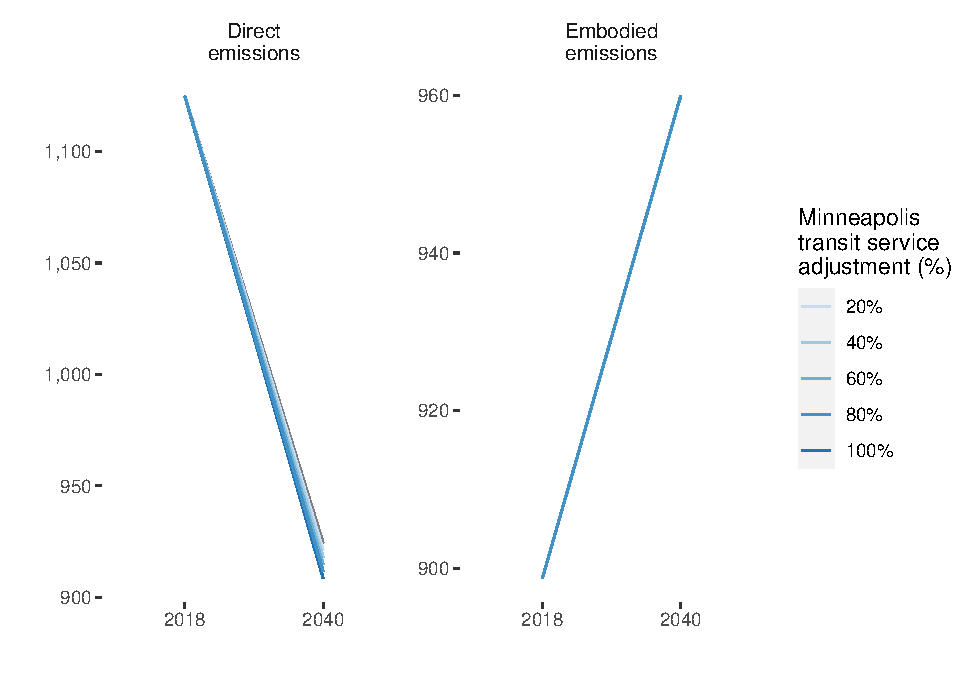
\includegraphics{_main_files/figure-latex/fig-transitservice-1.pdf}

\begin{verbatim}
## Joining, by = "Mode"
\end{verbatim}

\label{tab:tab-transit-comp}Emissions in tonnes CO2e - 60\% increase in transit service Minneapolis

Mode

2018 Baseline

2040 Business-as-Usual

2040 Scenario

Bike

0.00

0.00

0.00

School bus

1.01

1.33

1.33

Urban bus (standard, non-BRT bus)

50.70

51.72

72.41

Passenger light duty vehicle

1,069.93

883.89

849.84

Intercity rail

0.17

0.18

0.25

Urban rail

3.78

4.49

6.28

Walk

0.00

0.00

0.00

\hypertarget{telework}{%
\subsection{Telework}\label{telework}}

The most recent studies that also include energy associated with working from home find a effective reduction of 2.5-2.8\% in household CO2 emissions per day. (\protect\hyperlink{ref-Kim_Choo_Mokhtarian_2015}{Kim, Choo, and Mokhtarian 2015})

A scenario factor (SF) can be introduced to the generic GHG impact equation as an adjustment based on the effect of telework on both transportation and building energy.

At a first approximation, telework eliminates commute VMT. However, the net effect on VMT and household GHG production is less clear. Individuals who work from home tend to make additional non-commute trips during their additional discretionary time (\protect\hyperlink{ref-Mokhtarian_2009}{Mokhtarian 2009}) Other household members also can use the now available vehicle for their commute (potentially switching away from transit) or for other trips.

Finally, working from home introduces additional requirements on household energy consumption: more daytime heating and, potentially, the need for a larger dwelling to provide space for a home office. The most recent studies that also include energy associated with working from home find an effective reduction of 2.5-2.8\% in household CO2 emissions per telework day. (\protect\hyperlink{ref-fuEnvironmentalPolicyImplications2012a}{Fu et al. 2012})

An important secondary question regarding telework is its market potential. It is estimated that about 35 percent of jobs in the United States can be performed from home full-time (\protect\hyperlink{ref-Dingel_Neiman_2020}{Dingel and Neiman 2020}). Prior to the COVID-19 pandemic, time use data for the United States indicates that less than a quarter of workers worked from home, and most spent less than half their working hours at home. The portion of jobs that can be done from home varies by metropolitan area. In MSP, approximately 38 to 52 percent of jobs can be done fully through telework (\protect\hyperlink{ref-Dingel_Neiman_2020}{Dingel and Neiman 2020}).

We estimate a 2.75\% decrease in personal vehicle miles traveled for each person-day of telework.

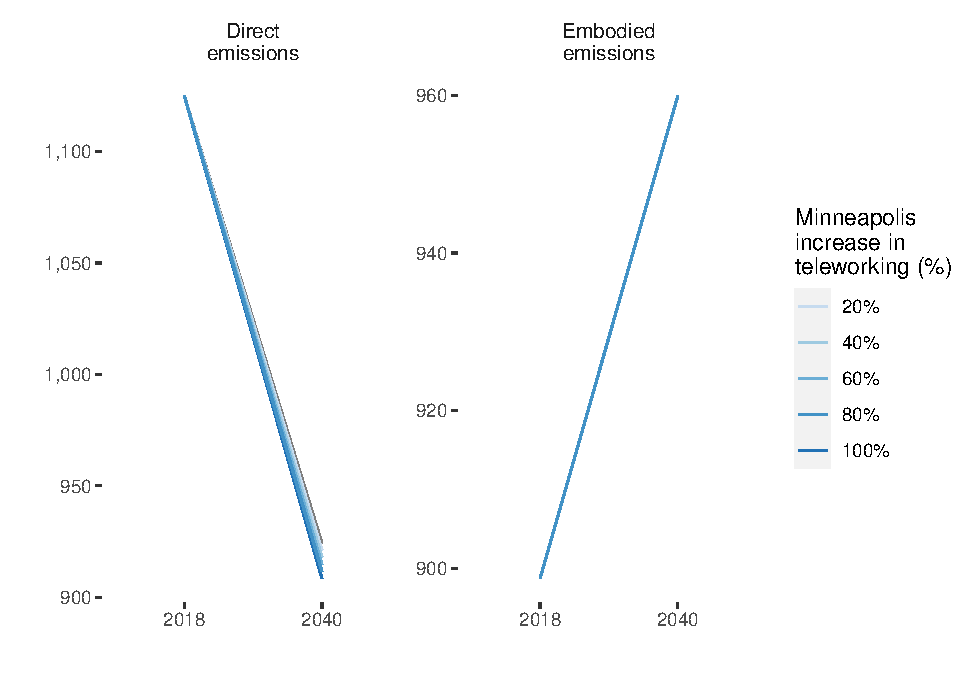
\includegraphics{_main_files/figure-latex/fig-telework-1.pdf}

\begin{verbatim}
## Joining, by = "Mode"
\end{verbatim}

\label{tab:tab-telework-comp}Emissions in tonnes CO2e - 60\% increase in people teleworking Minneapolis

Mode

2018 Baseline

2040 Business-as-Usual

2040 Scenario

Bike

0.00

0.00

0.00

School bus

1.01

1.33

1.33

Urban bus (standard, non-BRT bus)

50.70

51.72

51.72

Passenger light duty vehicle

1,069.93

883.89

857.03

Intercity rail

0.17

0.18

0.18

Urban rail

3.78

4.49

4.49

Walk

0.00

0.00

0.00

\hypertarget{road-pricing}{%
\subsection{Road Pricing}\label{road-pricing}}

In the future, road pricing will likely be an essential component of transportation policy. Road pricing is key for automated vehicles and dynamic ride-sharing policies because it helps address the increased vehicle miles traveled projected to occur with adopting these technologies. Furthermore, road pricing provides an alternative revenue stream to the gas tax as vehicle efficiency increases and electric vehicle adoption grows.

The scenario planning model includes three alternatives for road pricing. The first is a vehicle miles traveled (VMT) fee that charges for each mile of travel. The second is a pay-as-you-drive insurance plan. Finally, the model includes a representation of congestion pricing. Ideally, congestion price should vary between the time of day and road link based on the current congestion level, but this is unfeasible to model. Instead, an elevated VMT fee is applied to a portion of travel, approximating the percent of congested VMT. Credit-based congestion pricing is recommended as a revenue-neutral strategy to address equity in road pricing. It provides credits to travelers who shift their travel model or departure time.

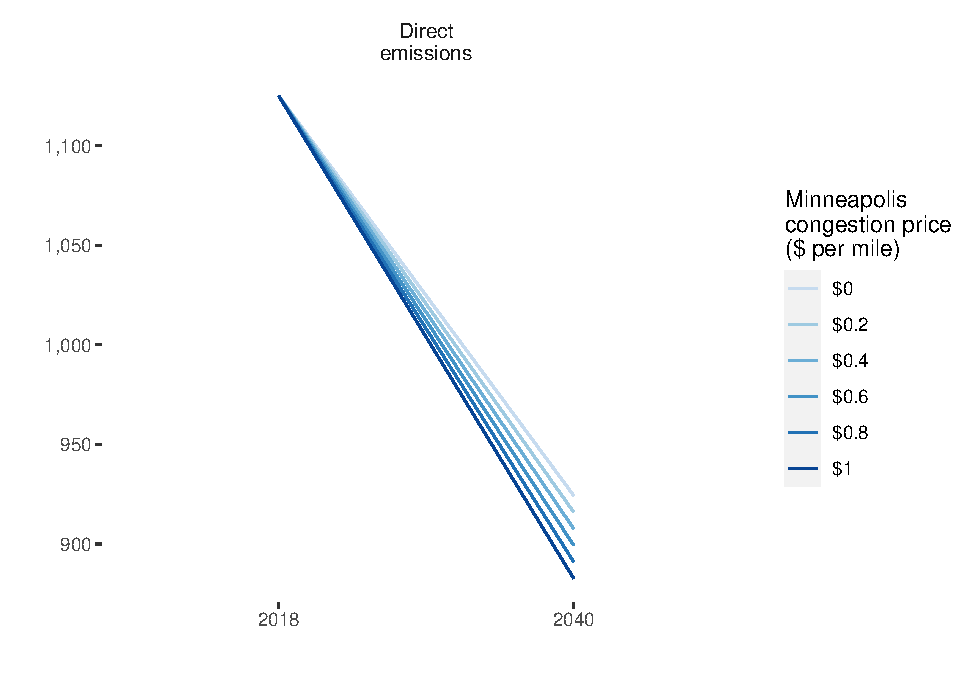
\includegraphics{_main_files/figure-latex/fig-roadprice-1.pdf}

\begin{verbatim}
## Joining, by = "Mode"
\end{verbatim}

\label{tab:tab-rp-comp}Emissions in tonnes CO2e - \$1 per mile congestion price Minneapolis

Mode

2018 Baseline

2040 Business-as-Usual

2040 Scenario

Bike

0.00

0.00

0.00

School bus

1.01

1.33

1.33

Urban bus (standard, non-BRT bus)

50.70

51.72

55.17

Passenger light duty vehicle

1,069.93

883.89

821.13

Intercity rail

0.17

0.18

0.19

Urban rail

3.78

4.49

4.79

Walk

0.00

0.00

0.00

\hypertarget{parking-policy}{%
\subsection{Parking Policy}\label{parking-policy}}

Parking is an important component of the transportation system. A lack of parking can result in additional VMT from vehicles searching for a parking spot (up to 30\% of vehicles in downtown traffic (\protect\hyperlink{ref-shoupCruisingParking2006}{Shoup 2006})). Surface lots and parkades take up valuable space that could be put to more useful purposes.

The most common strategies for controlling parking demand are increasing its price and restricting the time that parking is available. These strategies have been reviewed in detail and price elasticities are available for the price of parking on VMT (see Table \ref{tab:tab-parking-price-effects}).

The long-run elasticity of VMT to parking cost is estimated to be in the range of -0.18 to -0.45, with a mean of 0.07 based on a meta-analysis of values reported in the literature (\protect\hyperlink{ref-lehnerPriceElasticityParking2019}{Lehner and Peer 2019}).

\begin{equation}
adj_{park} = 1 + \frac{price_{y}}{price_{y = 2018}} \times elast_{park_{m}} 
(\#eq:parking_price_adj)
\end{equation}

\(price_y\) is the price of parking on dollars per hour in year \(y\)\\
\(price_{y = 2018}\) is the price of parking in dollars per hour in 2018\\
\(elast_{park}\) is the elasticity or effect size of parking price increase on travel mode \(m\).

Values derived from TRACE (\protect\hyperlink{ref-TRACE_1999}{1999}) and referenced in Litman (\protect\hyperlink{ref-litmanUnderstandingTransportDemands2021}{2021}) and Lehner and Peer (\protect\hyperlink{ref-lehnerPriceElasticityParking2019}{2019}).

\setlength{\LTpost}{0mm}
\begin{longtable}{lrr}
\toprule
Mode & Increase in parking price relative to baseline & Effect on miles traveled by 2050 \\ 
\midrule
Automobile & +10\% & -7\% \\ 
Walking and cycling & +10\% & +3\% \\ 
Transit & +10\% & +1\% \\ 
\bottomrule
\end{longtable}
\begin{minipage}{\linewidth}
TRACE 1999\\
\end{minipage}

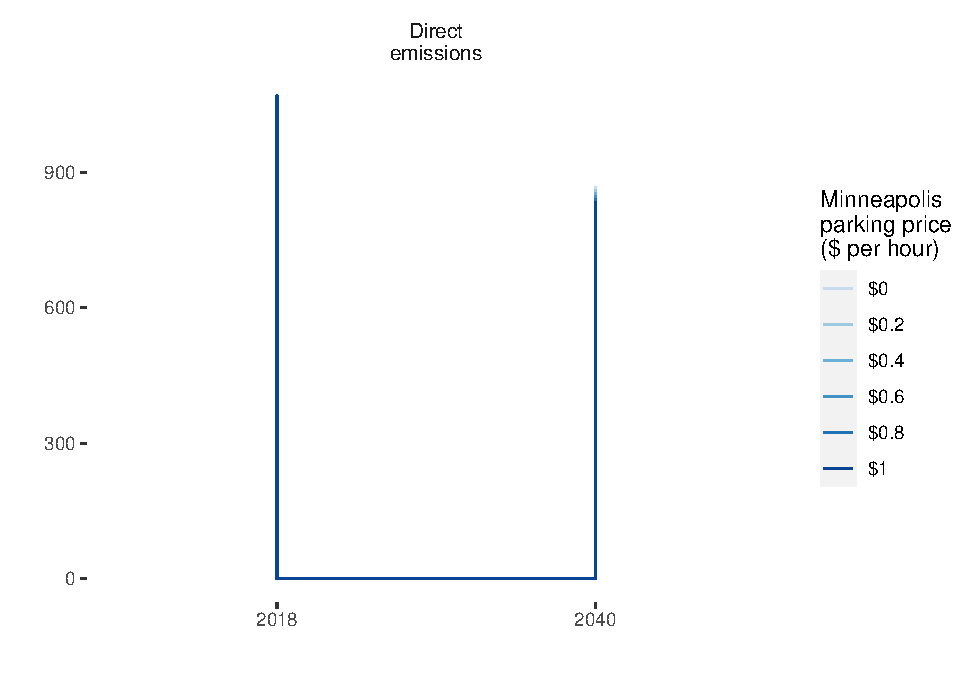
\includegraphics{_main_files/figure-latex/fig-parkingprice-1.pdf}

\hypertarget{land-use-and-forestry}{%
\chapter{Land Use and Forestry}\label{land-use-and-forestry}}

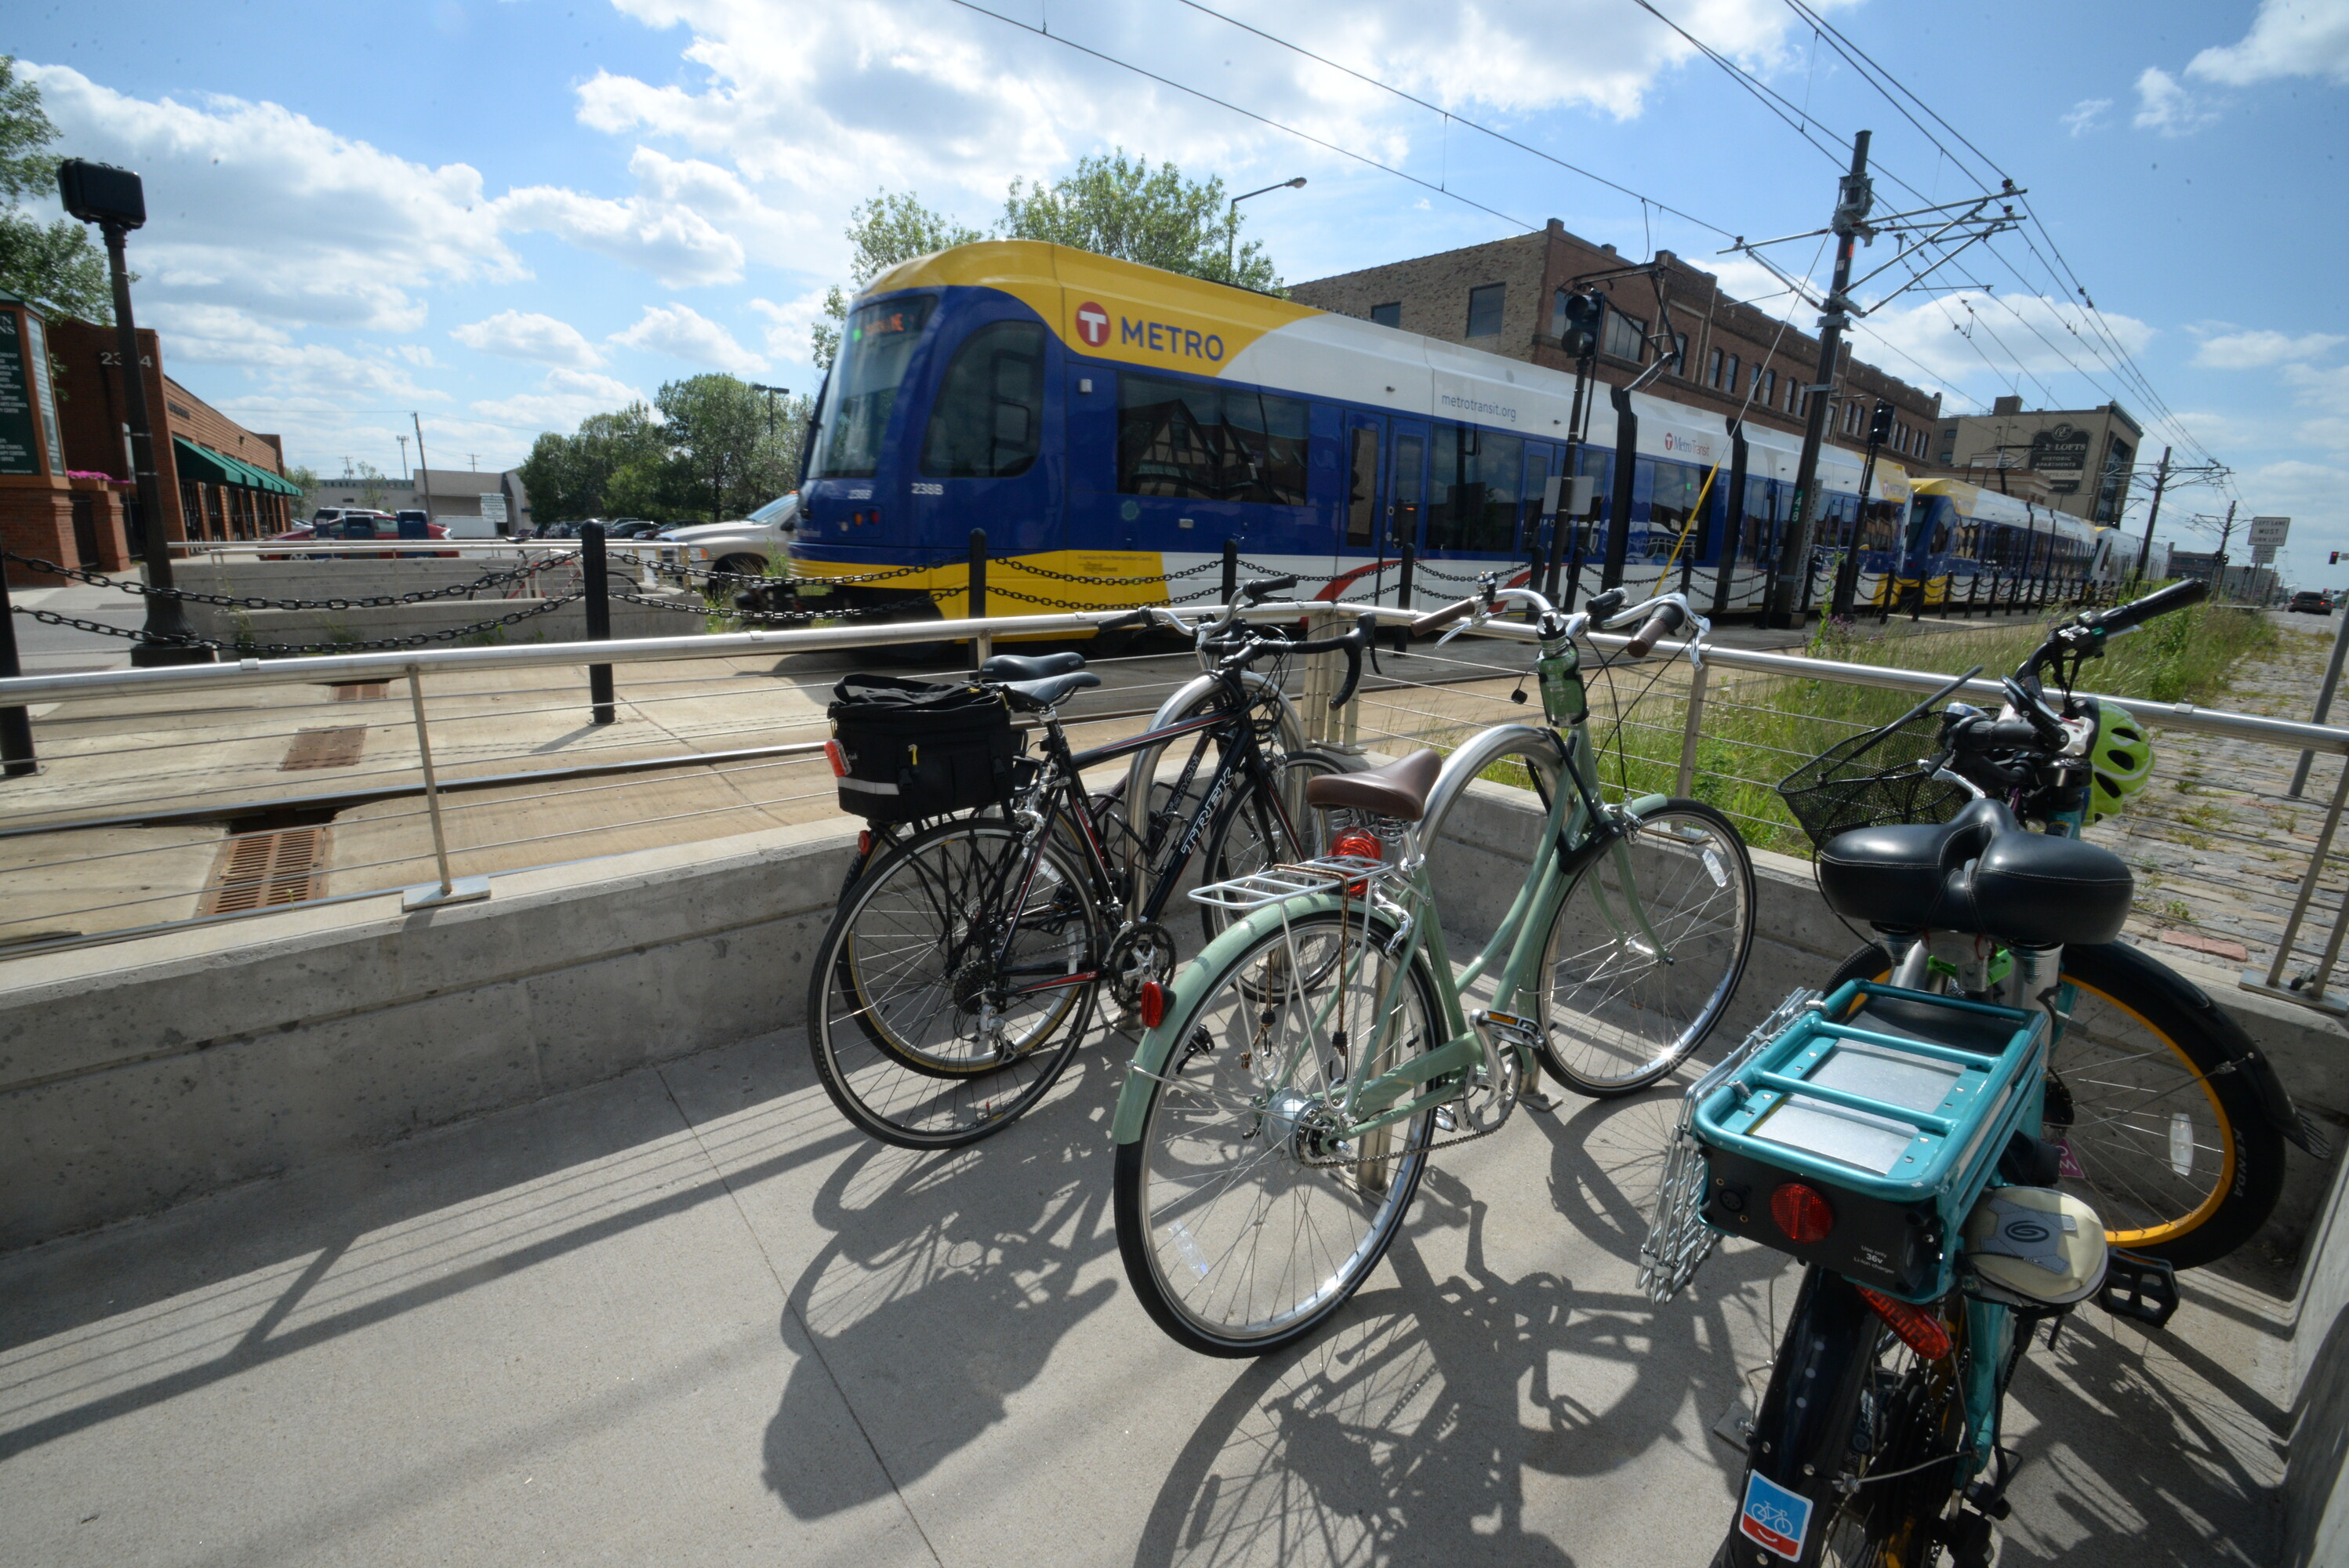
\includegraphics{images//2724.jpg}

Communities are taking steps to reduce their carbon footprint and address the impacts of climate change through a variety of measures, such as reducing energy consumption, promoting compact land use patterns, decreasing dependence on cars, and incorporating natural resources into development patterns. This approach, known as green infrastructure, enhances the resilience of the built environment, reduces emissions, and improves quality of life. These measures help communities prepare for the increasing frequency of extreme weather events and other climate impacts, safeguarding their resources and competitiveness.

Land use changes can release carbon stored in land, for instance, when urban impervious surfaces, like asphalt roads and residential areas, spread onto lands previously covered by forests or agriculture. This leads to net carbon emissions from land. On the other hand, significant urban reforestation can result in carbon storage in land, through soil and woody biomass, which can result in net carbon sequestration (negative emissions).

\hypertarget{framework-2}{%
\section{Framework}\label{framework-2}}

The impact of these effects can be modeled through satellite imagery and analysis of remote sensing data of urban land use changes planned by cities. Cities should aim to reduce their outward expansion through compact development and increase urban carbon storage through reforestation, as described in the guide on Urban Reforestation. Other strategies like soil conservation on agricultural land within the Metropolitan Council region can also contribute, although they were found to be relatively minor in the scenario planning model.

To outline the methodology for evaluating the impact of various land use and green infrastructure strategies, it is crucial to comprehend that each land cover type within our region, be it forested or impervious, possesses a distinct multiplier for carbon sequestration and carbon stocks. With the utilization of satellite imagery to acquire information on the region's land cover, we are able to make informed speculations regarding the potential for changes in land use and cover to augment or decrease greenhouse gas emissions.

The land freed up from impervious surfaces provides opportunities for nature-based solutions that can mitigate carbon and enhance climate resilience, as well as improve subjective well-being. To evaluate the impact of various land use and green infrastructure strategies, it is important to understand that each land cover type within the region, whether it be forested or impervious, has a unique multiplier for carbon sequestration and carbon stocks. By using satellite imagery to gather information on the region's land cover, informed assumptions can be made about the potential for changes in land use and cover to increase or decrease greenhouse gas emissions.

\hypertarget{land-cover-baseline-and-forecast}{%
\subsection{Land Cover Baseline and Forecast}\label{land-cover-baseline-and-forecast}}

A high-resolution land cover map for the Metropolitan Council region for the year 2016 was generated using support vector machine image classification on \emph{Planet RapidEye 5m Imagery}. This classification was merged with the 2019 edition of the \href{https://www.usgs.gov/centers/eros/science/national-land-cover-database}{National Land Cover Database} to create a 12-class land cover map. For more information on the image classification methodology, see (\protect\hyperlink{ref-Milnar_Ramaswami_2020}{Milnar and Ramaswami 2020}).

\label{tab:tab-land-cover-by-land-use}Land Cover Hectares for Minneapolis

Type

2016 {[}Baseline{]}

2040 {[}Busines-as-Usual{]}

Agriculture

40.66

84.39

Barren

157.13

147.86

Forest

205.90

343.63

Grass

1,012.95

1,035.19

Grassland

82.66

258.32

Impervious

7,995.26

7,719.22

Parking Lot

978.74

842.09

Shrub

0.94

1.38

Trees

3,471.62

3,485.43

Water

0.00

0.00

Wetland

12.55

41.48

Woody Wetland

19.79

19.21

\hypertarget{land-use-baseline-and-forecast}{%
\subsection{Land Use Baseline and Forecast}\label{land-use-baseline-and-forecast}}

The 2016 land use baseline data has been derived from the \href{https://metrocouncil.org/Data-and-Maps/Research-and-Data/Metadata/Landuse-Hist-Research.aspx}{Metropolitan Council Generalized Land Use}\footnote{The Metropolitan Council has been regularly creating generalized land use plans for the Twin Cities region since 1984 to fulfill its legal obligations and aid in long-term planning for the area. The Council utilizes this land use information to track growth and assess shifting patterns in land usage for various urban purposes. To plan for future needs and financing of Metropolitan services, such as Transit and Wastewater Services, the Council combines the land use trend data with its projections of households and jobs. In collaboration with local government units, the land use and forecast data are also used to assess expansions of the Metropolitan Urban Service Area (MUSA).} geospatial layer for all cities and townships. This data has been divided into three categories based on land use type: \emph{Urban Infill}, \emph{Exurban Development}, and \emph{Urban Expansion}.

\emph{Exurban Development} encompasses the following land use types: Undeveloped, Park/Recreation/Preserve, Agriculture, or Farmstead. All other land use types were categorized as \emph{Urban Infill} in the baseline data.

\begin{Shaded}
\begin{Highlighting}[]
\NormalTok{fig\_05\_land\_use}
\end{Highlighting}
\end{Shaded}

(\#tab:tab5.2)Land Use Hectares for Minneapolis

Variables

2018 {[}Baseline{]}

2040 {[}Busines-as-Usual{]}

Agricultural

9.20

8.93

Airport

2.96

2.87

Extractive

0.00

0.00

Farmstead

0.00

0.00

Golf Course

213.49

207.13

Industrial and Utility

1,075.95

1,109.74

Institutional

1,153.58

1,040.25

Major Highway

540.96

524.83

Major Railway

256.50

248.85

Manufactured Housing Park

0.00

0.00

Mixed Use Commercial

79.23

91.52

Mixed Use Industrial

113.81

117.38

Mixed Use Residential

130.29

131.25

Multifamily

780.74

786.49

Office

202.83

234.29

Open Water

0.00

0.00

Park, Recreational, or Preserve

1,423.53

1,381.11

Railway

0.00

725.74

Retail and Other Commercial

628.29

0.00

Seasonal Vacation

0.00

0.00

Single Family Attached

1,059.27

1,067.07

Single Family Detached

5,990.57

5,993.18

Undeveloped

317.01

307.56

\hypertarget{carbon-sequestration-and-carbon-stock}{%
\subsection{Carbon Sequestration and Carbon Stock}\label{carbon-sequestration-and-carbon-stock}}

\begin{Shaded}
\begin{Highlighting}[]
\NormalTok{carbon\_stocks\_and\_sequestration }\SpecialCharTok{\%\textgreater{}\%}
  \FunctionTok{rename}\NormalTok{(}
    \StringTok{"Land Cover Type"} \OtherTok{=}\NormalTok{ land\_cover\_type,}
    \StringTok{"Sequestration (mg C/ha/year)"} \OtherTok{=}\NormalTok{ sequest\_mg\_c\_per\_hectare\_per\_year,}
    \StringTok{"Stock (mg C/ha/year)"} \OtherTok{=}\NormalTok{ stock\_mg\_c\_per\_hectare}
\NormalTok{  ) }\SpecialCharTok{\%\textgreater{}\%}
  \FunctionTok{tableformat}\NormalTok{(}\AttributeTok{.caption =} \FunctionTok{paste0}\NormalTok{(}\StringTok{"General Carbon Values"}\NormalTok{))}
\end{Highlighting}
\end{Shaded}

\label{tab:unnamed-chunk-33}General Carbon Values

Land Cover Type

Sequestration (mg C/ha/year)

Stock (mg C/ha/year)

Impervious

0.00

33

Grass

-0.42

77

Trees

-1.30

115

Water

0.00

0

Barren

-0.01

0

Forest

-0.62

115

Shrub

-0.29

77

Grassland

-0.42

77

Agriculture

-0.19

41

Woody Wetland

-0.62

117

Wetland

-1.50

297

Parking Lot

0.00

33

\hypertarget{urban-form}{%
\subsection{Urban Form}\label{urban-form}}

In the coming decades, the Twin Cities region is expected to experience significant growth, with its population projected to increase from just under 3.2 million residents to over 3.7 million by 2040. This growth will bring about substantial changes in land use and land cover, particularly in the north and west suburbs.

\textbf{What are Biogenic Emissions?}

\emph{Biogenic emissions} arise from natural processes, predominantly the decomposition of organic matter. Urban expansion can have a significant
impact on these emissions, as the expansion itself can release long-stored carbon, and the presence of vegetation and soil can sequester carbon dioxide. However, the duration of carbon sequestration in biomass and the level at which it becomes saturated remain unclear.

To assess the impact of urban vegetation on carbon stock changes and sequestration, the method outlined in (\protect\hyperlink{ref-Milnar_Ramaswami_2020}{Milnar and Ramaswami 2020}) was used
to calculate these values for the study period of 2018-2040.

\textbf{\emph{About this strategy}} Our assumption is that cities can control (or at least influence)\ldots{}

\textbf{GHG Impact Calculation}

\[CO_2sqlc = (\text{Sequestration} + \text{Land Cover Change}) × 44/12\]
\emph{Where:}

\(\text{Sequestration} = \sum{(Ai × SRi)}\)\\
\(\text{Land Cover Change} = \sum{(Ait-1 × CDi ) - (Ait × CDi )]}\)

\emph{And:}

\begin{itemize}
\tightlist
\item
  \(\text{Sequestration} = \text{annual net sequestration from vegetation for a given city}\)
\item
  \(\text{Land Cover Change = annual organic carbon stock change from land conversion for a given city, averaged over the study period}\)
\item
  \(44/12 = \text{factor to convert Mg C to Mg } CO_2e\)
\item
  \(Ai = \text{Area of vegetation of cover type i (ha)}\)
\item
  \(SRi = \text{Annual net sequestration rate for cover type i. (Mg C ha-1 yr-1)}\)
\item
  \(CDi = \text{Carbon stock density factor for vegetation in cover type i (Mg C ha-1)}\)
\item
  \(i = 1 ,2, 3, ...n\) \(\text{land cover types}\)
\item
  \(t = \text{year for which biogenic emissions were calculated and compared to Scope 1+2 emissions for each city}\)
\end{itemize}

**** results coming soon\ldots{}

\hypertarget{conservation-tillage}{%
\subsection{Conservation Tillage}\label{conservation-tillage}}

Conventional agricultural practices, such as annual plowing, loosen the soil in preparation for planting. However, this can result in soil particles being exposed to wind and erosion, causing a loss of soil nutrients and organic matter over time. It is estimated that cultivated soils have lost 50-70\% of their soil carbon stock due to this method. To combat this, conservation tillage practices, such as no-till or reduced-till agriculture, have been introduced to minimize topsoil disturbance and reduce the loss of nutrients and organic matter in the soil. However, the impact of conservation tillage on greenhouse gas emissions is uncertain.

Conservation tillage has two main effects on greenhouse gas emissions:

\begin{enumerate}
\def\labelenumi{\arabic{enumi})}
\tightlist
\item
  By minimizing soil disturbance, the soil is able to retain a higher amount of organic carbon, reaching a new equilibrium.
\item
  By reducing plowing, there is a lower consumption of fossil fuels from farm equipment.
\end{enumerate}

In Minnesota, conservation tillage initiatives have been established by a variety of stakeholders, including the state and federal government, private sector companies, environmental advocacy groups, and academia. As a result, nearly half of all Minnesota counties growing corn and soy have at least 25\% of planted acres using reduced tillage practices, while about a quarter of the counties have at least 25\% of planted acres using no-till practices, according to the Crop Residue Management Survey.

\textbf{GHG Impact Calculation}

\[ \text{Conservation Tillage Avoided Emissions} = (C+T) × A \]
\emph{Where:}

\begin{itemize}
\item
  \(C\): Increased Biogenic Carbon Stock (Mg CO2/ha). Baseline soil organic carbon (SOC) stock is 41 Mg C/ha. It has been estimated that SOC content can increase from 1\% up to 1.54\% under conservation tillage2, thus carbon content can be increased from an average of 41 Mg C/ha to 63 Mg C/ha. This increase was assumed to increase over a period of 20 years. Whether the sequestration is maintained is highly uncertain.
\item
  \(T\): Avoided emissions from tractor fossil fuel use (Mg CO2/ha). The Natural Resources Conservation Service estimates no-till agriculture can reduce tractor fuel consumption by 3.2 gallons/acre6. Emissions from reduced fuel use were computed using a wells-to-wheels emissions factor7
\item
  \(A\): Area in Conservation Tillage (ha): The baseline area of no-till agriculture as reported in the 2017 USDA Census of Agriculture and this amount is changed for each scenario.
\end{itemize}

** results coming soon\ldots{}

\hypertarget{reduced-parking-area}{%
\subsection{Reduced Parking Area}\label{reduced-parking-area}}

in progress\ldots{}

\hypertarget{urban-tree-planting}{%
\subsection{Urban Tree Planting}\label{urban-tree-planting}}

Trees in urban areas have a high concentration of carbon stored in their canopies and are often the largest source of biogenic carbon in an urban ecosystem. By increasing the tree canopy in cities, it is possible to offset some carbon emissions and also provide other benefits, such as reducing energy costs for cooling and improving subjective well-being.

A mature urban forest can hold up to 115 Mg of carbon per hectare. Additionally, a tree that grows for one year can sequester carbon annually at a rate of 1.27 Mg of carbon per hectare per year. Both of these processes are included in the scenario planning model, which shows that urban reforestation can contribute significantly to a carbon sink, provided there is enough land for reforestation. This is likely to be more feasible in suburban communities than in central cities. However, it is important to note that urban trees grow quickly but may also die young. As a result, to maximize the potential carbon mitigation from urban reforestation, careful tree management and an understanding of the life cycle of urban forestry is necessary.

Many initiatives have been launched globally, including the Trillion Trees Initiative, which aims to restore forests in order to slow down climate change. Some cities, such as Los Angeles, have also launched projects to plant large numbers of trees, with the \emph{Los Angeles Million Trees Plan} estimating that up to 2.5 million trees could potentially be planted in the city. Recently, the City of Tucson announced a plan to plant one million trees by 2030.

In addition to mitigating the effects of climate change through carbon storage in woody biomass, urban trees offer a wide range of benefits, such as reducing the energy consumption of buildings, reducing urban heat, and improving subjective well-being. However, there are few empirical models to quantify the effect on building energy use, and existing data from St.~Paul suggests that the effect may be small compared to the carbon sink effect. Additionally, several studies have shown socio-economic inequality in tree canopy coverage, making equity an essential consideration in the spatial planning of urban reforestation.

\textbf{GROWING SHADE}

The Metropolitan Council, in partnership with the Nature Conservancy and the Tree Trust, has developed an online application called Growing Shade to help communities track and prioritize tree planting in areas with thin tree canopies. The app uses data from multiple sources, such as demographic information about neighborhoods, locations of businesses, schools, and parks, to create a detailed picture of a city at the neighborhood level. Nonprofits, cities, and communities can use the data to identify the best locations to plant trees, which can help to address issues such as high asthma rates, extreme temperatures, and the legacy of racial injustices.

\textbf{GHG Impact Calculation}

\[ \text{Sequestered Carbon (in Mg CO_2 e)} = CD × A × 11/3 \]
\emph{Where:}

\begin{itemize}
\tightlist
\item
  \(CD\) = Carbon stock density of urban trees in Mg/ha, a factor of aboveground biomass, (44.1 Mg C/ha, Nowak et al 2013), and belowground biomass to one meter (71 Mg C/ha, Pouyat et al.~20065) for a total stock density of 115.1 Mg C /ha.
\item
  \(A\) = Increased area of tree canopy under tree planting scenarios, in hectares.
\item
  \(11/3\) = Factor to convert Mg C to Mg CO2
\end{itemize}

\textbf{RESOURCES}

\begin{itemize}
\tightlist
\item
  \href{https://www.dnr.state.mn.us/forestry/urban/bmps.html}{Minnesota Department of Natural Resources: Urban forestry best management practices}
\item
  \href{https://extension.umn.edu/tree-selection-and-care/recommended-trees-minnesota}{University of Minnesota Extension: Recommended trees for Minnesota}
\item
  \href{https://www.minnesotamasternaturalist.org/docs/invasive_blitz/native_urban_trees_of_se_mn.pdf}{University of Minnesota Extension: Native urban trees of Southeast Minnesota}
\item
  \href{https://cities4forests.com/lg-urban-forests/introduction-to-policy-for-urban-forests/}{Cities4Forests: Introduction to policy for urban forests}
\end{itemize}

\emph{Additional Information}

\begin{itemize}
\tightlist
\item
  \href{http://www.treebenefits.com/calculator/}{National Tree Benefit Calculator}
\item
  \href{https://www.minneapolisparks.org/park_care__improvements/trees/}{Minneapolis Parks: Trees and the urban forest}
\item
  \href{https://www.dnr.state.mn.us/forestry/urban/tree-city-usa-awards.html\#cities}{2020 Tree City USA Communities in Minnesota}
\item
  \href{https://www.nrs.fs.fed.us/data/urban/state/?state=MN}{USDA: Urban forest data for Minnesota}
\end{itemize}

\textbf{EXAMPLES}

Several cities are investing in large-scale tree planting programs as a means of decarbonization, including the Trillion Trees Initiative, the City of Los Angeles, the City of Tucson, and the City of Pittsburgh. In Minnesota, the City of Saint Paul 2011 Urban Canopy Assessment explored the potential for large-scale tree planting within the city.

\textbf{GROWING SHADE}

The Metropolitan Council, in partnership with the Nature Conservancy and the Tree Trust, has developed an online application called Growing Shade to help communities track and prioritize tree planting in areas with thin tree canopies. The app uses data from multiple sources, such as demographic information about neighborhoods, locations of businesses, schools, and parks, to create a detailed picture of a city at the neighborhood level. Nonprofits, cities, and communities can use the data to identify the best locations to plant trees, which can help to address issues such as high asthma rates, extreme temperatures, and the legacy of racial injustices.

\hypertarget{conclusion}{%
\chapter{Conclusion}\label{conclusion}}

conclusion\ldots{}

\hypertarget{appendix}{%
\chapter*{Appendix}\label{appendix}}
\addcontentsline{toc}{chapter}{Appendix}

\hypertarget{building-energy-1}{%
\section{Building Energy}\label{building-energy-1}}

\hypertarget{energy-efficiency-strategies}{%
\subsection{Energy Efficiency Strategies}\label{energy-efficiency-strategies}}

\hypertarget{equations}{%
\subsubsection{Equations}\label{equations}}

\textbf{GHG Impact Calculation for Increased Multifamily Housing}

Calculate floor area changes:

\[ \text{new }sqft_{2040}^{sf} = units_{2040}^{sf} - units_{2018}^{sf} * x * (\bar{sqft}_{2040}^{sf} - \bar{sqft}_{2040}^{mf})\]
\emph{Where:}

\begin{itemize}
\tightlist
\item
  \(x\text{, where } 0 \le x \le 1\): The percentage of new single-family homes that are converted to multifamily homes
\item
  \(units_{2018}^{sf}\): The number of single-family housing units in the community in 2018
\item
  \(units_{2040}^{sf}\): The projected number of single-family housing units in the community in 2040
\item
  \(sqft_{2040}^{sf}\): The projected total floor area of single-family homes in the community in 2040
\item
  \(\bar{sqft}_{2040}^{sf}\): The projected average floor area of single-family homes in the community in 2040
\item
  \(\bar{sqft}_{2040}^{mf}\): The projected average floor area of multifamily homes in the community in 2040
\end{itemize}

Calculate new emissions:

\[\text{new total }kgCO_2e^{sf}_{2040} = \text{new }sqft_{2040}^{sf} * \left( \frac{MWh_{2040}^{residential}}{sqft_{2040}^{residential}} * \frac{kgCO2e}{MWh_{2040}} + \frac{therm_{2040}^{residential}}{sqft_{2040}^{residential}} * \frac{kgCO2e}{therm_{2040}} \right)\]

\emph{Where:}

\begin{itemize}
\tightlist
\item
  \(MWh_{2040}^{residential}/sqft_{2040}^{residential}\): Projected residential electricity use intensity per floor area in 2040
\item
  \(therm_{2040}^{residential}/sqft_{2040}^{residential}\): Projected residential natural gas use intensity per floor area in 2040
\item
  \(kgCO2e/MWh\) = The projected electricity emission factor in 2040
\item
  \(kgCO_2e/therms_{2040}\): The projected emissions factor of natural gas in 2040
\end{itemize}

\textbf{GHG Impact Calculation for Floor Area Reduction}

Calculate new floor area:

\[\text{new }sqft_{2040}^{sf}  = (units_{2040}^{sf} - units_{2018}^{sf}) * 0.5 * \left(\bar{sqft}_{2040}^{sf}-(1+x) * \bar{sqft}_{2018}^{sf}\right)\]
\[\text{where } 0 \le x \le 1\]

\emph{Where:}

\begin{itemize}
\tightlist
\item
  \((1+x)\): The rate of growth in single-family floor area in square feet per year.
\item
  \(sqft_{2040}^{sf}\): The total floor area of single-family homes in the community in 2040.
\item
  \(units_{2040}^{sf}\): The number of single-family housing units in the community in 2040.
\item
  \(units_{2018}^{sf}\): The number of single-family housing units in the community in 2018.
\item
  \(0.5\): This factor represents the assumption that half of the population will reduce the living space of new single-family homes in response to doubling energy prices.
\item
  \(\bar{sqft}_{2040}^{sf}\): The average floor area of single-family homes in the community in 2040.
\item
  \(\bar{sqft}_{2018}^{sf}\): The average floor area of single-family homes in the community in 2018.
\end{itemize}

Calculate new emissions:

\[\text{new total }kgCO_2e^{sf}_{2040} = \text{new }sqft_{2040}^{sf} *  \left( \frac{MWh_{2040}^{residential}}{sqft_{2040}^{residential}} * \frac{kgCO2e}{MWh_{2040}} + \frac{therm_{2040}^{residential}}{sqft_{2040}^{residential}} * \frac{kgCO2e}{therm_{2040}} \right)\]

\emph{Where:}

\begin{itemize}
\tightlist
\item
  \(MWh_{2040}^{residential}/sqft_{2040}^{residential}\): The projected residential electricity use intensity per floor area in 2040
\item
  \(therm_{2040}^{residential}/sqft_{2040}^{residential}\): The projected residential natural gas use intensity per floor area in 2040
\item
  \(kgCO2e/MWh\) = The projected electricity emission factor in 2040
\item
  \(kgCO_2e/therms_{2040}\): The projected emissions factor of natural gas in 2040
\end{itemize}

\textbf{GHG Impact Calculation for New Home Efficiency}

Calculate new efficency:

\[\text{new } sqft_{2040}^{sf} = x * (units_{2040}^{sf}-units_{2018}^{sf}) * \bar{sqft}_{2040}^{sf} * 0.64\]

\emph{Where:}

\begin{itemize}
\tightlist
\item
  \(x \text{, where } 0 \le x \le 1\): The percentage of new single family homes that are LEED Gold
\item
  \(sqft_{2040}^{sf}\): The total floor area of single-family homes in the community in 2040
\item
  \(units_{2040}^{sf}\): The number of single-family housing units in the community in 2040
\item
  \(units_{2018}^{sf}\): The number of single-family housing units in the community in 2018
\item
  \(\bar{sqft}_{2040}^{sf}\): The average floor area of single-family homes in the community in 2040
\item
  \(0.64\): This factor represents the reduction in energy use intensity due to highly-efficient LEED Gold construction
\end{itemize}

Calculate new emissions:

\[\text{new total }kgCO_2e^{sf}_{2040} = \text{new }sqft_{2040}^{sf} * \left( \frac{MWh_{2040}^{residential}}{sqft_{2040}^{residential}} * \frac{kgCO2e}{MWh_{2040}} + \frac{therm_{2040}^{residential}}{sqft_{2040}^{residential}} * \frac{kgCO2e}{therm_{2040}} \right)\]

\emph{Where:}

\begin{itemize}
\tightlist
\item
  \(MWh_{2040}^{residential}/sqft_{2040}^{residential}\): The projected residential electricity use intensity per floor area in 2040
\item
  \(therm_{2040}^{residential}/sqft_{2040}^{residential}\): The projected residential natural gas use intensity per floor area in 2040
\item
  \(kgCO2e/MWh\) = The projected electricity emission factor in 2040
\item
  \(kgCO_2e/therms_{2040}\): The projected emissions factor of natural gas in 2040
\end{itemize}

\textbf{GHG Impact Calculation for Existing Home Efficiency}

Calculate new floor area:

\[\text{new }sqft_{2040}^{sf+mf} = (units_{2018}^{sf} * x * 0.33 * \bar{sqft}_{2018}^{sf} + units_{2018}^{mf} * x * 0.33 * \bar{sqft}_{2018}^{mf})\]

\emph{Where:}

\begin{itemize}
\tightlist
\item
  \(x \text{, where } 0 \le x \le 1\): The percentage of existing homes to be retrofitted, defaulted to 80\%
\item
  \(0.33\): The percent reduction in energy use intensity due to efficiency gains of the retrofitting.
\item
  \(units_{2040}^{sf}\): The number of single-family housing units in 2018
\item
  \(units_{2018}^{mf}\): The number of multifamily homes in 2018
\item
  \(\bar{sqft}_{2018}^{sf}\): The average floor area of single-family homes in 2018
\item
  \(\bar{sqft}_{2018}^{mf}\): The average floor area of multi-family homes in 2018
\end{itemize}

Calculate new emissions:

\[\text{new total }kgCO_2e^{sf + mf}_{2040} = \text{new }sqft_{2040}^{sf + mf}  * \left( \frac{MWh_{2040}^{residential}}{sqft_{2040}^{residential}} * \frac{kgCO2e}{MWh_{2040}} + \frac{therm_{2040}^{residential}}{sqft_{2040}^{residential}} * \frac{kgCO2e}{therm_{2040}} \right))\]

\emph{Where:}

\begin{itemize}
\tightlist
\item
  \(MWh_{2040}^{residential}/sqft_{2040}^{residential}\): The projected residential electricity use intensity per floor area in 2040
\item
  \(therm_{2040}^{residential}/sqft_{2040}^{residential}\): The projected residential natural gas use intensity per floor area in 2040
\item
  \(kgCO2e/MWh\) = The projected electricity emission factor in 2040
\item
  \(kgCO_2e/therms_{2040}\): The projected emissions factor of natural gas in 2040
\end{itemize}

\textbf{GHG Impact Calculation for Behavior Change}

Calculate new floor area:

\[ \text{new }sqft_{2040}^{residential} = \text{new }sqft_{2040}^{sf+mf} = x * pop_{2040} * \frac{sqft_{2040}^{sf + mf}}{pop_{2040}} * 0.11 \]

\emph{Where:}

\begin{itemize}
\tightlist
\item
  \(x \text{, where } 0 \le x \le 1\): The percentage of homes that change their behavior for energy efficiency.
\item
  \(0.11\): The percentage reduction in household energy use as a result of smart nudges.
\item
  \(pop_{2040}\): The total population in 2040.
\item
  \(sqft_{2040}^{sf+mf}/population_{2040}\): The average square footage per person in 2040 for residential buildings.
\end{itemize}

Calculate new emissions:

\[\text{new total }kgCO_2e^{residential}_{2040} = \text{new }sqft_{2040}^{residential}* \left( \frac{MWh_{2040}^{residential}}{sqft_{2040}^{residential}} * \frac{kgCO2e}{MWh_{2040}} + \frac{therm_{2040}^{residential}}{sqft_{2040}^{residential}} * \frac{kgCO2e}{therm_{2040}} \right)\]
\emph{Where:}

\begin{itemize}
\tightlist
\item
  \(MWh_{2040}^{residential}/sqft_{2040}^{residential}\): The projected residential electricity use intensity per floor area in 2040
\item
  \(therm_{2040}^{residential}/sqft_{2040}^{residential}\): The projected residential natural gas use intensity per floor area in 2040
\item
  \(kgCO2e/MWh\) = The projected electricity emission factor in 2040
\item
  \(kgCO_2e/therms_{2040}\): The projected emissions factor of natural gas in 2040
\end{itemize}

\textbf{GHG Impact Calculation for Clean Residential Energy}

Calculate electricity use in 2040:

\[
\text{Busines as Usual }MWh_{2040}^{residential} = pop_{2040} * \frac{sqft_{2040}^{residential}}{pop_{2040}} * \frac{MWh}{sqft_{2040}^{residential}}
\]

\emph{Where:}

\begin{itemize}
\tightlist
\item
  \(pop_{2040}\): The projected population in 2040
\item
  \(sqft_{2040}^{residential}/pop_{2040}\): The projected residential floor area per capita in 2040
\item
  \(MWh/sqft_{2040}^{residential}\): The projected residential electricity per floor area in 2040
\end{itemize}

Calculate new emissions:

\[\text{new electricity }kgCO_2e^{residential}_{2040} = \text{Busines as Usual }MWh_{2040}^{residential} *  \frac{kgCO2e}{MWh_{2040}} * (1-x) \]

\emph{Where:}

\begin{itemize}
\tightlist
\item
  \((1-x) \text{, where } 0 \le x \le 1\): The percentage reduction in the emissions of the electric grid
\item
  \(kgCO2e/MWh\) = The projected electricity emission factor in 2040
\end{itemize}

\textbf{GHG Impact Calculation for Electrifying Residential Heat}

Natural Gas for Space Heating:

\[term_1 = \left(pop_{2040} * \frac{sqft_{2040}^{residential}}{pop_{2040}} * \frac{therm_{2040}^{residential}}{sqft_{2040}^{residential}} \right) * x * \frac{kgCO2e}{therm_{2040}} * 71\% \]
\[\text{space heating natural gas }kgCO_2e_{2040}^{residential} = term_1 - \left(term_1 * (0.8/5.02) * \frac{0.0293therm}{MWh}\right) * \frac{kgCO_2e}{MWh_{2040}}\]

Natural Gas for Water Heating:

\[term_2 = \left(pop_{2040} * \frac{sqft_{2040}^{residential}}{pop_{2040}} * \frac{therm_{2040}^{residential}}{sqft_{2040}^{residential}} \right) * x * \frac{kgCO2e}{therm_{2040}} * 24\% \]
\[\text{water heating natural gas }kgCO_2e_{2040}^{residential} = term_2 - \left(term_2 * 100\% * \frac{0.0293therm}{MWh}\right) * \frac{kgCO_2e}{MWh_{2040}}\]

\emph{Where:}

\begin{itemize}
\tightlist
\item
  \(x\): The percentage of additional households with heating electrified, defaulted to be 59\% - 14\% of homes already electrified
\item
  \(pop_{2040}\): The projected population in 2040
\item
  \(71\%\): Assumed natural gas for space heating
\item
  \(24\%\): Assumed natural gas for water heating
\item
  \(100\%\): The ratio of natural gas water heating to electric water heating
\item
  \((0.8/5.02)\): The ratio of boiler efficiency to heat pump efficiency
\item
  \(sqft_{2040}^{residential}/pop_{2040}\): The projected residential floor area per capita in 2040
\item
  \(0.0293therm/MWh\): The conversion factor from therm to MWH
\item
  \(kgCO_2e/MWh_{2040}\): The projected emissions factor of electricity in 2040
\end{itemize}

\textbf{Policy Approaches}

\begin{itemize}
\tightlist
\item
  \href{https://naphnetwork.org/policymaker-resources/}{The Passive House Network: Policymaker Resources Overview}
\end{itemize}

\textbf{Financing}

\begin{itemize}
\tightlist
\item
  \href{https://www.mncee.org/residential-statewide-lending}{Minnesota Center for Energy and the Environment: Home energy improvement loans.}
\item
  \href{https://mn.gov/commerce/consumers/consumer-assistance/weatherization/}{State of Minnesota Weatherization Assistance Program: The Weatherization Assistance Program provides free home energy upgrades to income-eligible homeowners and renters to help save energy.}
  *\href{https://mn.gov/commerce/consumers/consumer-assistance/energy-assistance/}{State of Minnesota Energy Assistance Program: The Energy Assistance Program (EAP) helps pay home heating costs and furnace repairs for income-qualified households.}
\end{itemize}

\textbf{Additional Information}

\begin{itemize}
\item
  \href{https://www.edockets.state.mn.us/EFiling/edockets/searchDocuments.do?method=showPoup\&documentId=\%7B40BC0B73-0000-C918-8CE1-D182E3E20EED\%7D\&documentTitle=20207-164492-01}{Xcel Energy Minnesota Electric and Natural Gas Conservation Improvement Program: 2021-2023 CIP Triennial Plan}
\item
  \href{https://www.imt.org/resources/map-u-s-building-benchmarking-policies/}{Institute for Market Transformation: Map of US cities, counties, and states with mandatory building energy benchmarking and transparency policies for existing buildings}
\item
  \href{https://passivehouseminnesota.org/passive-house/}{Passive House Minnesota}
\item
  \href{https://passivehouse.com/}{Passive House Institute}
\item
  \href{https://passivehouse-database.org/index.php?lang=en\#k_minnesota}{Passive House database}
\item
  Equity considerations: Tong, K., Ramaswami, A., Xu, C., et al.~(2021). Measuring social equity in urban energy use and interventions using fine-scale data. PNAS, 118 (24), e2023554118. \url{https://doi.org/10.1073/pnas.2023554118}.
\end{itemize}

\hypertarget{increased-multifamily-strategy}{%
\subsection{Increased Multifamily Strategy}\label{increased-multifamily-strategy}}

\begin{itemize}
\tightlist
\item
  \href{https://metrocouncil.org/Handbook/Plan-Elements/Housing.aspx}{Metropolitan Council Local Planning Handbook: Housing}
\item
  \href{https://metrocouncil.org/Housing/Planning/HOUSING-POLICY-PLAN-2040/2040-Housing-Policy-Plan.aspx}{Metropolitan Council Thrive MSP 2040: Housing Policy Plan}
\item
  \href{https://metrocouncil.org/Data-and-Maps/Publications-And-Resources/MetroStats/Construction-Activity/On-the-Rise-New-Residential-Construction-in-the-T.aspx}{MetroStats: On the rise: New residential construction in the Twin Cities Region}
\end{itemize}

\textbf{Policy Approaches}

\begin{itemize}
\tightlist
\item
  \href{https://www.aceee.org/multifamily-project}{American Council for an Energy-Efficient Economy: The multifamily energy savings project}
\item
  \href{https://www.brookings.edu/policy2020/bigideas/to-improve-housing-affordability-we-need-better-alignment-of-zoning-taxes-and-subsidies/}{Brookings Institution: Policy recommendations for housing affordability}
\end{itemize}

\hypertarget{electrification}{%
\subsection{Electrification}\label{electrification}}

\textbf{Additional Information}

\begin{itemize}
\tightlist
\item
  \href{https://www.mncee.org/air-source-heat-pumps}{Minnesota Center for Energy and the Environment: Air source heat pumps}
\item
  \href{https://www.mnashp.org/for-homeowners}{Minnesota Air Source Heat Pump Collaborative: Case studies}
\item
  \href{https://concordma.gov/2776/Heat-Pump-Case-Studies}{Town of Concord, Massachusetts: Case studies}
\end{itemize}

\textbf{Policy Approaches}

\begin{itemize}
\tightlist
\item
  \href{https://environmentamerica.org/sites/environment/files/reports/Electric-Buildings-2021/National-Electric-Buildings-Web.pdf?_ga=2.10624308.1239172724.1638808751-1075536878.1638808751\#page=32}{Environment America: Policy recommendations for electric buildings}
\item
  \href{https://www.aceee.org/sites/default/files/pdfs/programs_to_electrify_space_heating_brief_final_6-23-20.pdf}{American Council for an Energy-Efficient Economy: Programs to electrify space heating in homes and buildings}
\item
  \href{https://ipu.msu.edu/wp-content/uploads/2018/04/LBNL-Electrification-of-Buildings-2018.pdf\#page=47}{Lawrence Berkeley National Laboratory: Policy approaches to enable electrification}
\end{itemize}

\textbf{Financing}

\begin{itemize}
\tightlist
\item
  \href{https://www.mncee.org/residential-statewide-lending}{Minnesota Center for Energy and the Environment: Home energy improvement loans}
\end{itemize}

\hypertarget{renewable-natural-gas-2}{%
\subsection{Renewable Natural Gas}\label{renewable-natural-gas-2}}

\textbf{Policy Approaches}

\begin{itemize}
\tightlist
\item
  \href{https://www.wri.org/research/renewable-natural-gas-climate-strategy-guidance-state-policymakers}{World Resources Institute: Renewable Natural Gas as a Climate Strategy: Guidance for State Policymakers}
\item
  \href{https://www.eesi.org/papers/view/fact-sheet-biogasconverting-waste-to-energy}{Environmental and Energy Study Institute: Fact Sheet \textbar{} Biogas: Converting Waste to Energy}
\item
  \href{https://www.epa.gov/agstar/guidelines-and-permitting-livestock-anaerobic-digesters}{US Environmental Protection Agency: Guidelines and Permitting for Livestock Anaerobic Digesters}
\end{itemize}

\textbf{Case Studies}

\begin{itemize}
\tightlist
\item
  \href{https://www.anl.gov/es/reference/renewable-natural-gas-database}{Argonne National Laboratory: Renewable Natural Gas Database}
\item
  \href{https://www.mda.state.mn.us/manure-digester-case-study-haubenschild-farm}{Haubenschild Dairy Manure Digester, Princeton, MN}
\item
  \href{https://www.epa.gov/lmop/webinar-case-study-university-california-renewable-natural-gas-projects}{US EPA: Case study of University of California renewable natural gas projects}
\end{itemize}

\textbf{Additional Information}

\begin{itemize}
\tightlist
\item
  \href{https://www.epa.gov/anaerobic-digestion/basic-information-about-anaerobic-digestion-ad}{US Environmental Protection Agency: Basic information about anaerobic digestion}\\
\item
  \href{https://www.mda.state.mn.us/environment-sustainability/manure-digesters}{MN Department of Agriculture: Manure digesters}
\item
  \href{https://research.umn.edu/inquiry/post/drawing-renewable-resources-organic-waste}{University of Minnesota: Drawing renewable resources from organic waste}
\end{itemize}

\hypertarget{transportation-1}{%
\section{Transportation}\label{transportation-1}}

\hypertarget{data-sources}{%
\subsection{Data sources}\label{data-sources}}

The transportation module is constructed based on a set of standard forecasts for inputs such as passenger miles traveled, vehicle miles traveled, existing vehicle stock, new vehicle sales, average vehicle occupancy, fuel efficiency, and population. These parameters are utilized to predict the vehicle miles traveled and resultant emissions. The scenario planning tool then utilizes selected intervention elasticities and proportional effects to calculate the potential reduction in emissions.

\begin{longtable}{ll}
\toprule
Measure & Source \\ 
\midrule
\multicolumn{2}{l}{Passenger light duty vehicle} \\ 
\midrule
Total stock of vehicles & MA3T; 2019 Travel Behavior Inventory \\ 
Spark ignition (gasoline) stock & MA3T; 2019 Travel Behavior Inventory \\ 
Compression ignition (diesel) stock & MA3T; 2019 Travel Behavior Inventory \\ 
Hybrid electric vehicle stock & MA3T; 2019 Travel Behavior Inventory \\ 
Plug-in hybrid electric vehicle stock & MA3T; 2019 Travel Behavior Inventory \\ 
Battery electric vehicle stock & MA3T; 2019 Travel Behavior Inventory \\ 
Proportion of plug-in hybrid electric vehicle miles traveled operated in electric mode & EV vehicle range; 2019 Travel Behavior Inventory \\ 
Total existing vehicles & MA3T; 2019 Travel Behavior Inventory \\ 
Existing gasoline vehicles & MA3T; 2019 Travel Behavior Inventory \\ 
Existing diesel vehicles & MA3T; 2019 Travel Behavior Inventory \\ 
Existing hybrid electric vehicles & MA3T; 2019 Travel Behavior Inventory \\ 
Existing plug-in hybrid electric vehicles & MA3T; 2019 Travel Behavior Inventory \\ 
Existing battery electric vehicles & MA3T; 2019 Travel Behavior Inventory \\ 
Total vehicle sales & MA3T; 2019 Travel Behavior Inventory \\ 
Total gasoline vehicle sales & MA3T; 2019 Travel Behavior Inventory \\ 
Total diesel vehicle sales & MA3T; 2019 Travel Behavior Inventory \\ 
Total hybrid electric sales & MA3T; 2019 Travel Behavior Inventory \\ 
Total plug-in hybrid electric sales & MA3T; 2019 Travel Behavior Inventory \\ 
Total battery electric sales & MA3T; 2019 Travel Behavior Inventory \\ 
Average vehicle occupancy & FHWA; 2019 Travel Behavior Inventory \\ 
Passenger miles traveled & Metropolitan Council Travel Demand Model \\ 
Parking cost & 2019 Travel Behavior Inventory \\ 
Spark ignition (gasoline) fuel economy & U.S. Energy Information Administration \\ 
Compression ignition (diesel) fuel economy & U.S. Energy Information Administration \\ 
Hybrid electric fuel economy & U.S. Energy Information Administration \\ 
Plug-in hybrid electric fuel economy in gasoline mode & U.S. Energy Information Administration \\ 
Plug-in hybrid electric economy in electric mode & Pl<9a>tz, Moll, Li, et. al. 2020 \\ 
Battery electric vehicle electricity conusmption & Brooker, Gonder, Wang et. al., 2015 \\ 
\midrule
\multicolumn{2}{l}{Active transportation (walk and bike)} \\ 
\midrule
Passenger miles traveled & Metropolitan Council Travel Demand Model \\ 
\midrule
\multicolumn{2}{l}{Urban bus (standard, non-BRT bus)} \\ 
\midrule
Total stock of vehicles & Metro Transit Facts series; National Transit Database \\ 
Biodiesel bus stock & Metro Transit Facts series; National Transit Database \\ 
Hybrid electric vehicle stock & Metro Transit Facts series; National Transit Database \\ 
Battery electric vehicle stock & Metro Transit Facts series; National Transit Database \\ 
Total existing vehicles & Metro Transit Facts series; National Transit Database \\ 
Biodiesel bus existing stock & Metro Transit Facts series; National Transit Database \\ 
Existing hybrid electric vehicles & Metro Transit Facts series; National Transit Database \\ 
Existing battery electric vehicles & Metro Transit Facts series; National Transit Database \\ 
Total vehicle sales & Metro Transit Facts series; National Transit Database \\ 
Biodiesel bus sales & Metro Transit Facts series; National Transit Database \\ 
Total hybrid electric sales & Metro Transit Facts series; National Transit Database \\ 
Total battery electric sales & Metro Transit Facts series; National Transit Database \\ 
Average vehicle occupancy & FHWA \\ 
Passenger miles traveled & Metropolitan Council Travel Demand Model \\ 
Biodiesel bus fuel economy, miles per gallon & O'Dea, 2018 \\ 
Hybrid electric fuel economy & O'Dea, 2018 \\ 
Battery electric vehicle electricity conusmption & National Transit Database \\ 
\midrule
\multicolumn{2}{l}{Bus rapid transit} \\ 
\midrule
Total stock of vehicles & Metro Transit Facts series; National Transit Database \\ 
Biodiesel bus stock & Metro Transit Facts series; National Transit Database \\ 
Hybrid electric vehicle stock & Metro Transit Facts series; National Transit Database \\ 
Battery electric vehicle stock & Metro Transit Facts series; National Transit Database \\ 
Total existing vehicles & Metro Transit Facts series; National Transit Database \\ 
Biodiesel bus existing stock & Metro Transit Facts series; National Transit Database \\ 
Existing hybrid electric vehicles & Metro Transit Facts series; National Transit Database \\ 
Existing battery electric vehicles & Metro Transit Facts series; National Transit Database \\ 
Total vehicle sales & Metro Transit Facts series; National Transit Database \\ 
Biodiesel bus sales & Metro Transit Facts series; National Transit Database \\ 
Total hybrid electric sales & Metro Transit Facts series; National Transit Database \\ 
Total battery electric sales & Metro Transit Facts series; National Transit Database \\ 
Passenger miles traveled & Metropolitan Council Travel Demand Model \\ 
Biodiesel bus fuel economy, miles per gallon & O'Dea, 2018 \\ 
Hybrid electric fuel economy & O'Dea, 2018 \\ 
Battery electric vehicle electricity conusmption & National Transit Database \\ 
Average vehicle occupancy & Khani, Cao et. al., 2018 \\ 
\midrule
\multicolumn{2}{l}{Urban rail} \\ 
\midrule
Total stock of vehicles & Not measured \\ 
Stock of electric train vehicles & Not measured \\ 
Passenger miles traveled & Metropolitan Council Travel Demand Model \\ 
Electric vehicle electricity consumption for rail & National Transit Database \\ 
Average vehicle occupancy & Khani, Cao et. al., 2018 \\ 
\midrule
\multicolumn{2}{l}{Intercity rail} \\ 
\midrule
Total stock of vehicles & Not measured \\ 
Biodiesel bus stock & Not measured \\ 
Stock of electric train vehicles & Not measured \\ 
Passenger miles traveled & Metropolitan Council Travel Demand Model \\ 
Average vehicle occupancy & Khani, Cao et. al., 2018 \\ 
Biodiesel bus fuel economy, miles per gallon & National Transit Database \\ 
Electric vehicle electricity consumption for rail & National Transit Database \\ 
\midrule
\multicolumn{2}{l}{School bus} \\ 
\midrule
Passenger miles traveled & Metropolitan Council Travel Demand Model \\ 
Total stock of vehicles & Not measured \\ 
Compression ignition (diesel) stock & Not measured \\ 
Battery electric vehicle stock & Not measured \\ 
Compression ignition (diesel) fuel economy & Argonne National Laboratory; US Department of Energy \\ 
Battery electric vehicle electricity conusmption & Argonne National Laboratory; US Department of Energy \\ 
Average vehicle occupancy & Khani, Cao et. al., 2018 \\ 
\midrule
\multicolumn{2}{l}{Walk} \\ 
\midrule
Passenger miles traveled & Metropolitan Council Travel Demand Model \\ 
Average vehicle occupancy & Not measured \\ 
\midrule
\multicolumn{2}{l}{Bike} \\ 
\midrule
Passenger miles traveled & Metropolitan Council Travel Demand Model \\ 
Average vehicle occupancy & Not measured \\ 
\midrule
\multicolumn{2}{l}{Dynamic ride sharing} \\ 
\midrule
Population of the city or township unit & Metropolitan Council Travel Demand Model \\ 
NA & Haonan, Kockelman, and Gurumurthy, 2020 \\ 
Vehicle miles traveled per shared electric vehicle for dyanmic ride sharing & Haonan, Kockelman, and Gurumurthy, 2020 \\ 
Dynamic ride sharing share adjustment to translate across years & Haonan, Kockelman, and Gurumurthy, 2020 \\ 
\midrule
\multicolumn{2}{l}{Autonomous vehicle} \\ 
Autonomous vehicle share adjustment to translate across years & Huang, Kockelman, and Quarles, 2020; Taiebat, Stolper, and Wu, 2019 \\ 
\bottomrule
\end{longtable}

\hypertarget{source-summaries}{%
\subsubsection{Source summaries}\label{source-summaries}}

\hypertarget{ma3t-doc}{%
\paragraph{Market Acceptance of Advanced Automotive Technologies (MA3T)}\label{ma3t-doc}}

Model developed by Oak Ridge National Laboratory (ORNL) to simulate the diverse purchasing behaviors among individuals in the market place. You can read more about the model and find full documentation on the \href{https://teem.ornl.gov/ma3t.shtml}{ORNL website 
\includegraphics[width=0.88em,height=1em]{_main_files/figure-latex/fa-icon-1cb4dd6c25746ed6d3d2a87cd5fc3c74.pdf}}

\begin{Shaded}
\begin{Highlighting}[]
\NormalTok{knitr}\SpecialCharTok{::}\FunctionTok{include\_graphics}\NormalTok{(}\StringTok{"https://www.ornl.gov/sites/default/files/ma3t1.png"}\NormalTok{)}
\end{Highlighting}
\end{Shaded}

\begin{figure}
\includegraphics[width=0.7\linewidth]{https://www.ornl.gov/sites/default/files/ma3t1} \caption{MA3T model abstraction [@linMA3TModel2013]}\label{fig:ma3t-graphic}
\end{figure}

\hypertarget{metropolitan-council-sources}{%
\subsubsection{Metropolitan Council sources}\label{metropolitan-council-sources}}

\hypertarget{metc-tbi}{%
\paragraph{Travel Behavior Inventory (TBI)}\label{metc-tbi}}

The Travel Behavior Inventory (TBI) is a 10-year program by the Metropolitan Council. It includes a household travel survey, a survey of on-board transit riders, and other travel behavior data collection.

Key findings from the 2019 TBI can be found on the \href{https://metrocouncil.org/Transportation/Performance/Travel-Behavior-Inventory/2019.aspx}{Met Council website 
\includegraphics[width=0.88em,height=1em]{_main_files/figure-latex/fa-icon-1cb4dd6c25746ed6d3d2a87cd5fc3c74.pdf}}

\hypertarget{metc-travel-demand}{%
\paragraph{Travel Demand Model}\label{metc-travel-demand}}

The Met Council, like all large metropolitan planning organizations, maintains a regional transportation forecasting model. The model is used to forecast travel for all types of transportation and highway and transit facility usage.

The current regional travel demand forecast model is called an ``activity-based model'', which means that it simulates transportation decisions made by individuals ranging from long-term (e.g.~regular work/school location, whether to own an automobile), day-level (e.g, what activities to engage in, with whom, where, and when), and trip-level (what transportation mode to use, what route to take) in order to evaluate policy and investment choices at a high level of detail.

Other, more single-purpose forecast models are maintained by the Council as well, including a regional implementation of the FTA's STOPS model for transitway ridership forecasting, as well as a regional park-and ride model.

You can find more information on the \href{https://metrocouncil.org/Transportation/Performance/Travel-Forecasting.aspx}{Met Council website 
\includegraphics[width=0.88em,height=1em]{_main_files/figure-latex/fa-icon-1cb4dd6c25746ed6d3d2a87cd5fc3c74.pdf}}

\hypertarget{transit-facts}{%
\paragraph{Transit Facts}\label{transit-facts}}

\hypertarget{council-specific-studies}{%
\paragraph{Council-specific studies}\label{council-specific-studies}}

(\protect\hyperlink{ref-khaniStudyBusRapid2018}{Khani et al. 2018})

\hypertarget{federal-data-sources}{%
\subsubsection{Federal data sources}\label{federal-data-sources}}

\hypertarget{federal-highway-administration-fhwa}{%
\paragraph{Federal Highway Administration (FHWA)}\label{federal-highway-administration-fhwa}}

Average vehicle occupancy (\protect\hyperlink{ref-federalhighwayadministrationfhwaAverageVehicleOccupancy2018}{Federal Highway Administration (FHWA) 2018}).

\hypertarget{eia-sources}{%
\paragraph{US Energy Information Administration (EIA)}\label{eia-sources}}

\hypertarget{fuel-economies}{%
\subparagraph{Fuel economies}\label{fuel-economies}}

\hypertarget{aeo-values}{%
\subparagraph{Annual Energy Outlook values}\label{aeo-values}}

The Annual Energy Outlook (AEO) is a report series by the US Energy Information Administration (EIA) exploring long-term energy trends in the United States (\protect\hyperlink{ref-eiaAnnualEnergyOutlook2021}{{``Annual {Energy Outlook}''} 2021}).

You can read more on the \href{https://www.eia.gov/outlooks/aeo}{EIA website 
\includegraphics[width=0.88em,height=1em]{_main_files/figure-latex/fa-icon-1cb4dd6c25746ed6d3d2a87cd5fc3c74.pdf}}.

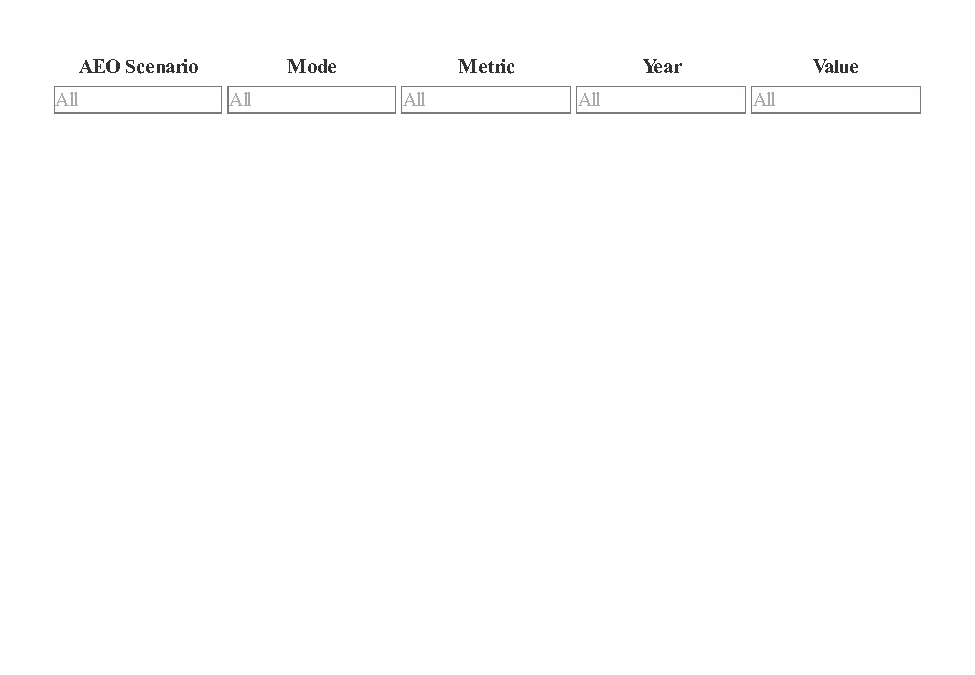
\includegraphics{_main_files/figure-latex/tab-aeo-values-1.pdf}

\hypertarget{ntd-source}{%
\paragraph{National Transit Database (NTD)}\label{ntd-source}}

\hypertarget{study-specific-values}{%
\subsubsection{Study-specific values}\label{study-specific-values}}

Brooker, Aaron, Jeffrey Gonder, Lijuan Wang, Eric Wood, Sean Lopp, and Laurie Ramroth. ``FASTSim: A Model to Estimate Vehicle Efficiency, Cost and Performance.'' SAE Technical Paper. Warrendale, PA: SAE International, April 14, 2015. \url{https://doi.org/10.4271/2015-01-0973}. (\protect\hyperlink{ref-brookerFASTSimModelEstimate2015}{Brooker et al. 2015})

Jimmy O'Dea, ``Electric Vs. Diesel Vs. Natural Gas: Which Bus Is Best for the Climate?'' Union of Concerned Scientists, 2018, \url{https://blog.ucsusa.org/jimmy-odea/electric-vs-diesel-vs-natural-gas-which-bus-is-best-for-the-climate} (\protect\hyperlink{ref-odeaElectricVsDiesel2018}{O'Dea 2018})

Haonan Yan, Kara M. Kockelman, and Krishna Murthy Gurumurthy, ``Shared Autonomous Vehicle Fleet Performance: Impacts of Trip Densities and Parking Limitations,'' Transportation Research Part D: Transport and Environment 89 (2020): 1--19, \url{https://doi.org/10.1016/j.trd.2020.102577}. (\protect\hyperlink{ref-yanSharedAutonomousVehicle2020}{Yan, Kockelman, and Gurumurthy 2020})

Huang, Yantao, Kara M. Kockelman, and Neil Quarles. ``How Will Self-Driving Vehicles Affect U.S. Megaregion Traffic? The Case of the Texas Triangle.'' Research in Transportation Economics 84 (2020): 1--18. \url{https://doi.org/10.1016/j.retrec.2020.101003}. (\protect\hyperlink{ref-huangHowWillSelfdriving2020}{Huang, Kockelman, and Quarles 2020})

Taiebat, Morteza, Samuel Stolper, and Ming Xu. ``Forecasting the Impact of Connected and Automated Vehicles on Energy Use A Microeconomic Study of Induced Travel and Energy Rebound.'' Applied Energy 247 (August 2019): 297--308. \url{https://doi.org/10.1016/j.apenergy.2019.03.174}. (\protect\hyperlink{ref-taiebatForecastingImpactConnected2019}{Taiebat, Stolper, and Xu 2019})

Patrick Plötz et al., ``Real-World Usage of Plug-in Hybrid Electric Vehicles,'' International Council on Clean Transportation (ICCT) White Paper, 2020 (\protect\hyperlink{ref-plotzRealworldUsagePlugin2020}{Plötz et al. 2020})

\hypertarget{transportation-modes}{%
\subsection{Transportation modes}\label{transportation-modes}}

\begin{longtable}{lll}
\toprule
Code & Description & Note \\ 
\midrule
BUS & Bus & bus \\ 
FRAIL & Freight rail & freight\_rail \\ 
FSHIP & Freight ship & Mostly barges going to port in St. Paul \\ 
HDT & Heavy duty vehicle & heavy\_duty\_veh \\ 
LDV & Light duty vehicle & light\_duty\_veh \\ 
MDT & Medium duty vehicle & medium\_duty\_veh \\ 
RAIL & Rail & rail \\ 
CUT & Combined unit truck & Eqivalent to HDT \\ 
SUT & Single unit truck & Equivalent to MDT \\ 
FR & Freight rail & NA \\ 
MM & Multi-modal freight (combination of truck and rail) & NA \\ 
AIR & Air freight & NA \\ 
WAT & Water freight & Equivalent to FSHIP \\ 
PLDV & Passenger light duty vehicle & NA \\ 
BU & Urban bus (standard, non-BRT bus) & NA \\ 
BRT & Bus rapid transit & NA \\ 
RU & Urban rail & LRT \\ 
RI & Intercity rail & Northstar commuter rail \\ 
BS & School bus & NA \\ 
DRS & Dynamic ride sharing & NA \\ 
AT & Active transportation (walk and bike) & NA \\ 
WALK & Walk & NA \\ 
BIKE & Bike & NA \\ 
AV & Autonomous vehicle & autonomous\_vehicle \\ 
\bottomrule
\end{longtable}

\hypertarget{emission-sources}{%
\subsection{Emission Sources}\label{emission-sources}}

\begin{longtable}{ll}
\toprule
Abbreviation & Description \\ 
\midrule
ER & Xcel energy reference scenario electricity generation mix \\ 
EM & Xcel energy mitigation scenario electricity generation mix \\ 
SI & Spark ignition \\ 
CI & Combustion Ignition \\ 
BCI & Biodiesel fuel consumed in thousands of gallons \\ 
SUTCI & Single-unit truck diesel fuel consumed in millions of gallons \\ 
CUTCI & Combined-unit truck diesel fuel consumed in millions of gallons \\ 
RCI & Rail diesel fuel consumed in millions of gallons \\ 
MMCI & Multi-modal diesel fuel consumed in millions of gallons \\ 
WCI & Water diesel fuel consumed in millions of gallons \\ 
ASI & Air spark ignition (jet fuel) fuel consumed in millions of gallons \\ 
SI-EMB & Spark ignition/gasoline embodied emissions from vehicle sales in thousands of mt CO2 \\ 
CI-EMB & Combustion ignition/diesel embodied emissions from vehicle sales in thousands of mt CO2 \\ 
HEV-EMB & HEV embodied emissions from vehicle sales in thousands of mt CO2 \\ 
PHEV-EMB & PHEV embodied emissions from vehicle sales in thousands of mt CO2 \\ 
BEV-EMB & BEV emodied emisisons from vehicle sales in thousands of mt CO2 \\ 
BU-BCI-EMB & Biodiesel bus embodied emissions from vehicle sales in thousands of mt CO2 \\ 
BU-HEV-EMB & HEV bus embodied emissions from vehicle sales in thousands of mt CO2 \\ 
BU-BEV-EMB & BEV bus embodied emissions from vehicle sales in thousands of mt CO2 \\ 
BS-CI-EMB & Diesel school bus embodied emissions from vehicle sales in thousands of mt CO2 \\ 
BS-BEV-EMB & BEV school bus embodied emissions from vehicle sales in thousands of mt CO2 \\ 
\bottomrule
\end{longtable}

\hypertarget{future-costs-per-mile}{%
\subsection{Future costs per mile}\label{future-costs-per-mile}}

\setlength{\LTpost}{0mm}
\begin{longtable}{l|r}
\toprule
\multicolumn{1}{l}{} & Cost per mile\textsuperscript{1} \\ 
\midrule
\multicolumn{2}{l}{Passenger} \\ 
\midrule
Light duty vehicle, gasoline & $\text{\$}0.62$ \\ 
Light duty vehicle, diesel & $\text{\$}0.62$ \\ 
Light duty vehicle, hybrid & $\text{\$}0.55$ \\ 
Light duty vehicle, plug-in hybrid & $\text{\$}0.49$ \\ 
Light duty vehicle, battery electric & $\text{\$}0.55$ \\ 
\midrule
\multicolumn{2}{l}{Transit, bus} \\ 
\midrule
Bus, diesel & $\text{\$}2.91$ \\ 
Bus, hybrid & $\text{\$}2.82$ \\ 
Bus, battery electric & $\text{\$}2.73$ \\ 
Bus rapid transit, diesel & $\text{\$}4.01$ \\ 
Bus rapid transit, hybrid & $\text{\$}3.88$ \\ 
Bus rapid transit, battery electric & $\text{\$}3.76$ \\ 
\midrule
\multicolumn{2}{l}{Transit, rail} \\ 
\midrule
Light-rail, electric & $\text{\$}4.45$ \\ 
Passenger rail, diesel & $\text{\$}4.43$ \\ 
Passenger rail, electric & $\text{\$}4.21$ \\ 
\midrule
\multicolumn{2}{l}{School bus} \\ 
\midrule
Diesel & $\text{\$}2.43$ \\ 
Battery electric & $\text{\$}2.28$ \\ 
\midrule
\multicolumn{2}{l}{Dynamic ride-sharing} \\ 
\midrule
Hybrid & $\text{\$}0.58$ \\ 
Plug-in hybrid & $\text{\$}0.52$ \\ 
Battery electric & $\text{\$}0.59$ \\ 
\bottomrule
\end{longtable}
\begin{minipage}{\linewidth}
\textsuperscript{1}2020 dollars\\
\end{minipage}

\hypertarget{forecasted-electricity-energy-mix}{%
\subsection{Forecasted Electricity Energy Mix}\label{forecasted-electricity-energy-mix}}

Reference and mitigation scenarios developed by Xcel Energy (\protect\hyperlink{ref-energyUpperMidwestIntegrated2020}{Xcel Energy 2020}).

\begin{Shaded}
\begin{Highlighting}[]
\CommentTok{\# energy\_mix \textless{}{-} readr::read\_csv("data/ghg\_factor\_forecast\_by\_scenario.csv",}
\CommentTok{\#   show\_col\_types = F}
\CommentTok{\# ) \%\textgreater{}\%}
\CommentTok{\#   mutate(across(3:11, \textasciitilde{} round(.x * 100, digits = 1)),}
\CommentTok{\#     source = stringr::str\_remove(source, "\textbackslash{}\textbackslash{}*"),}
\CommentTok{\#     scenario = paste0(scenario, " Scenario")}
\CommentTok{\#   )}
\CommentTok{\# \# tidyr::pivot\_longer(cols = 3:11,}
\CommentTok{\# \#                     names\_to = "year",}
\CommentTok{\# \#                     values\_to = "prop") \%\textgreater{}\%}
\CommentTok{\# \# mutate(year = stringr::str\_remove(year, "X") \%\textgreater{}\%}
\CommentTok{\# \#          as.numeric()) \%\textgreater{}\%}
\CommentTok{\# \# filter(year != 2018)}
\CommentTok{\#}
\CommentTok{\# energy\_mix \%\textgreater{}\%}
\CommentTok{\#   group\_by(scenario) \%\textgreater{}\%}
\CommentTok{\#   gt::gt(}
\CommentTok{\#     id = "energy{-}mix{-}forecast",}
\CommentTok{\#     caption = "Forecasted Electricity Generation Mix (\%)",}
\CommentTok{\#     rowname\_col = "source"}
\CommentTok{\#   ) \%\textgreater{}\%}
\CommentTok{\#   \# gt::tab\_stubhead("Scenario") \%\textgreater{}\%}
\CommentTok{\#   gt::tab\_source\_note("Xcel Energy, 2020") \%\textgreater{}\%}
\CommentTok{\#   gt::opt\_row\_striping(TRUE) \%\textgreater{}\%}
\CommentTok{\#   gt::tab\_footnote("Carbon{-}Free Generation includes utility{-}scale solar, onshore wind, biomass, hydro{-}electric, and nuclear generators",}
\CommentTok{\#     locations = gt::cells\_stub(rows = c(1, 6))}
\CommentTok{\#   ) \%\textgreater{}\%}
\CommentTok{\#   gt::tab\_options(row\_group.font.weight = "bold")}
\end{Highlighting}
\end{Shaded}

\hypertarget{land-use-1}{%
\section{Land Use}\label{land-use-1}}

\hypertarget{reforestation-strategy}{%
\subsection{Reforestation Strategy}\label{reforestation-strategy}}

\begin{itemize}
\tightlist
\item
  \href{https://www.dnr.state.mn.us/forestry/urban/bmps.html}{Minnesota Department of Natural Resources: Urban forestry best management practices}
\item
  \href{https://extension.umn.edu/tree-selection-and-care/recommended-trees-minnesota}{University of Minnesota Extension: Recommended trees for Minnesota}
\item
  \href{https://www.minnesotamasternaturalist.org/docs/invasive_blitz/native_urban_trees_of_se_mn.pdf}{University of Minnesota Extension: Native urban trees of Southeast Minnesota}
\item
  \href{https://cities4forests.com/lg-urban-forests/introduction-to-policy-for-urban-forests/}{Cities4Forests: Introduction to policy for urban forests}
\end{itemize}

\emph{Additional Information}

\begin{itemize}
\tightlist
\item
  \href{http://www.treebenefits.com/calculator/}{National Tree Benefit Calculator}
\item
  \href{https://www.minneapolisparks.org/park_care__improvements/trees/}{Minneapolis Parks: Trees and the urban forest}
\item
  \href{https://www.dnr.state.mn.us/forestry/urban/tree-city-usa-awards.html\#cities}{2020 Tree City USA Communities in Minnesota}
\item
  \href{https://www.nrs.fs.fed.us/data/urban/state/?state=MN}{USDA: Urban forest data for Minnesota}
\end{itemize}

\textbf{EXAMPLES}

Several cities are investing in large-scale tree planting programs as a means of decarbonization, including the Trillion Trees Initiative, the City of Los Angeles, the City of Tucson, and the City of Pittsburgh. In Minnesota, the City of Saint Paul 2011 Urban Canopy Assessment explored the potential for large-scale tree planting within the city.

\hypertarget{refs}{}
\begin{CSLReferences}{1}{0}
\leavevmode\vadjust pre{\hypertarget{ref-eiaAnnualEnergyOutlook2021}{}}%
{``Annual {Energy Outlook}.''} 2021. Government. {Washington DC}: {US Energy Information Administration}. \url{https://doi.org/10.1128/AAC.03728-14}.

\leavevmode\vadjust pre{\hypertarget{ref-brookerFASTSimModelEstimate2015}{}}%
Brooker, Aaron, Jeffrey Gonder, Lijuan Wang, Eric Wood, Sean Lopp, and Laurie Ramroth. 2015. {``{FASTSim}: {A Model} to {Estimate Vehicle Efficiency}, {Cost} and {Performance}.''} SAE Technical Paper 2015-01-0973. {Warrendale, PA}: {SAE International}. \url{https://doi.org/10.4271/2015-01-0973}.

\leavevmode\vadjust pre{\hypertarget{ref-Chester_Horvath_2009}{}}%
Chester, Mikhail V., and Arpad Horvath. 2009. \emph{Life-Cycle Energy and Emissions Inventories for Motorcycles, Diesel Automobiles, School Buses, Electric Buses, Chicago Rail, and New York City Rail}. \url{https://doi.org/10.11436/mssj.15.250}.

\leavevmode\vadjust pre{\hypertarget{ref-Dingel_Neiman_2020}{}}%
Dingel, Jonathan I, and Brent Neiman. 2020. {``How Many Jobs Can Be Done at Home?''} \emph{Journal of Public Economics} 189. \url{https://doi.org/10.1016/j.jpubeco.2020.104235}.

\leavevmode\vadjust pre{\hypertarget{ref-federalhighwayadministrationfhwaAverageVehicleOccupancy2018}{}}%
Federal Highway Administration (FHWA). 2018. {``Average {Vehicle Occupancy Factors} for {Computing Travel Time Reliability Measures} and {Total Peak Hour Excessive Delay Metrics}.''} Government. {Washington DC}. \url{https://www.fhwa.dot.gov/tpm/guidance/avo_factors.pdf}.

\leavevmode\vadjust pre{\hypertarget{ref-fuEnvironmentalPolicyImplications2012a}{}}%
Fu, Miao, James Kelly, J. Peter Clinch, and Fearghal King. 2012. {``Environmental Policy Implications of Working from Home: {Modelling} the Impacts of Land-Use, Infrastructure and Socio-Demographics.''} \emph{Energy Policy} 47 (August): 416--23. \url{https://doi.org/10.1016/j.enpol.2012.05.014}.

\leavevmode\vadjust pre{\hypertarget{ref-huangHowWillSelfdriving2020}{}}%
Huang, Yantao, Kara M. Kockelman, and Neil Quarles. 2020. {``How Will Self-Driving Vehicles Affect {U}.{S}. Megaregion Traffic? {The} Case of the {Texas Triangle}.''} \emph{Research in Transportation Economics} 84: 1--18. \url{https://doi.org/10.1016/j.retrec.2020.101003}.

\leavevmode\vadjust pre{\hypertarget{ref-khaniStudyBusRapid2018}{}}%
Khani, Alireza, Jason Cao, Benjamin Tomhave, Yufeng Zhang, John Hourdos, Peter Dirks, Jack Olsson, Tao Tao, and Xinyi Wu. 2018. {``After {Study} of the {Bus Rapid Transit} '{A Line}' {Impacts}.''} Government 2018001. Transitway {Impacts Research Program}. {Center for Transportation Studies}: {University of Minnesota}. \url{http://cts-d8resmod-prd.oit.umn.edu:8080/pdf/cts-18-24-mndot-2018-35.pdf}.

\leavevmode\vadjust pre{\hypertarget{ref-Kim_Choo_Mokhtarian_2015}{}}%
Kim, Seung Nam, Sangho Choo, and Patricia L. Mokhtarian. 2015. {``Home-Based Telecommuting and Intra-Household Interactions in Work and Non-Work Travel: {A} Seemingly Unrelated Censored Regression Approach.''} \emph{Transportation Research Part A: Policy and Practice} 80: 197--214. \url{https://doi.org/10.1016/j.tra.2015.07.018}.

\leavevmode\vadjust pre{\hypertarget{ref-lehnerPriceElasticityParking2019}{}}%
Lehner, Stephan, and Stefanie Peer. 2019. {``The Price Elasticity of Parking: {A} Meta-Analysis.''} \emph{Transportation Research Part A: Policy and Practice} 121 (March): 177--91. \url{https://doi.org/10.1016/j.tra.2019.01.014}.

\leavevmode\vadjust pre{\hypertarget{ref-litmanUnderstandingTransportDemands2021}{}}%
Litman, Todd. 2021. {``Understanding {Transport Demands} and {Elasticities}: {How Prices} and {Other Factors Affect Travel Behavior}.''} {Victoria, BC}: {Victoria Transport Policy Institute}. \url{http://www.vtpi.org/elasticities.pdf}.

\leavevmode\vadjust pre{\hypertarget{ref-lovedayTopPlugInHybrid2019}{}}%
Loveday, Steven. 2019. {``Top 8 {Plug-In Hybrid Vehicles With The Longest Electric Range}.''} \emph{Inside EVs}. \url{https://insideevs.com/features/377286/top-phevs-longest-electric-range/}.

\leavevmode\vadjust pre{\hypertarget{ref-millard-ballAutonomousVehicleParking2019}{}}%
Millard-Ball, Adam. 2019. {``The Autonomous Vehicle Parking Problem.''} \emph{Transport Policy} 75 (March): 99--108. \url{https://doi.org/10.1016/j.tranpol.2019.01.003}.

\leavevmode\vadjust pre{\hypertarget{ref-Milnar_Ramaswami_2020}{}}%
Milnar, Michael, and Anu Ramaswami. 2020. {``Impact of Urban Expansion and in Situ Greenery on Community-Wide Carbon Emissions: {Method} Development and Insights from 11 {US} Cities.''} \emph{Environmental Science \& Technology} 54 (24): 16086--96. \url{https://doi.org/10.1021/acs.est.0c02723}.

\leavevmode\vadjust pre{\hypertarget{ref-Mokhtarian_2009}{}}%
Mokhtarian, Patricia L. 2009. {``If Telecommunication Is Such a Good Substitute for Travel, Why Does Congestion Continue to Get Worse?''} \emph{Transportation Letters} 1 (1): 1--17. \url{https://doi.org/10.3328/TL.2009.01.01.1-17}.

\leavevmode\vadjust pre{\hypertarget{ref-odeaElectricVsDiesel2018}{}}%
O'Dea, Jimmy. 2018. {``Electric Vs. {Diesel} Vs. {Natural Gas}: {Which Bus} Is {Best} for the {Climate}?''} {The Equation}. July 19, 2018. \href{https://blog.ucsusa.org/jimmy-odea/electric-vs-diesel-vs-natural-gas-which-bus-is-best-for-the-climate\#:~:text=Battery\%20electric\%20buses\%20range\%20from,is\%20getting\%20cleaner\%20every\%20year.}{https://blog.ucsusa.org/jimmy-odea/electric-vs-diesel-vs-natural-gas-which-bus-is-best-for-the-climate\#:\textasciitilde:text=Battery electric buses range from,is getting cleaner every year.}

\leavevmode\vadjust pre{\hypertarget{ref-perez-lombard_review_2008}{}}%
Pérez-Lombard, Luis, José Ortiz, and Christine Pout. 2008. {``A Review on Buildings Energy Consumption Information.''} \emph{Energy and Buildings} 40 (3): 394--98. \url{https://doi.org/10.1016/j.enbuild.2007.03.007}.

\leavevmode\vadjust pre{\hypertarget{ref-plotzRealworldUsagePlugin2020}{}}%
Plötz, Patrick, Cornelius Moll, Yaoming Li, Georg Bieker, and Peter Mock. 2020. {``Real-World Usage of Plug-in Hybrid Electric Vehicles: {Fuel} Consumption, Electric Driving, and {CO2} Emissions.''} {The International Council on Clean Transportation}. \url{https://theicct.org/sites/default/files/publications/PHEV-white\%20paper-sept2020-0.pdf}.

\leavevmode\vadjust pre{\hypertarget{ref-porterCarbonFreeBoston2019}{}}%
Porter, Christopher, Xiao Yun (Jane) Chang, Cutler J Cleveland, Peter Fox-Penner, Michael J Walsh, Margaret Cherne-hendrick, Taylor Perez, Janet Atkins, Christopher Cook, and et al. 2019. {``Transportation {Technical Report} 2019.''} Carbon {Free Boston}. {Boston, MA, USA}: {Boston University Institute for Sustainable Energy}. \url{https://sites.bu.edu/cfb/carbon-free-boston-report-released/technical-reports/}.

\leavevmode\vadjust pre{\hypertarget{ref-ramaswamiReviewIntegratedUrban2020}{}}%
Ramaswami, Anu, Andrew Fang, and Samuel Tabory. 2020. {``A {Review} of {Integrated Urban Planning Tools} for {Greenhouse Gas Mitigation}.''} {Washington DC}: {Global Platform for Sustainable Cities}. \url{https://doi.org/10.1596/33784}.

\leavevmode\vadjust pre{\hypertarget{ref-santasieriPlanningTransitSupportiveDevelopment2014}{}}%
Santasieri, Colette. 2014. \emph{Planning for {Transit-Supportive Development}: {A Practitioner}'s {Guide Section} 5: {Local Planning} and {Transit-Supportive Development}}.

\leavevmode\vadjust pre{\hypertarget{ref-shoupCruisingParking2006}{}}%
Shoup, Donald C. 2006. {``Cruising for Parking.''} \emph{Transport Policy} 13 (6): 479--86. \url{https://doi.org/10.1016/j.tranpol.2006.05.005}.

\leavevmode\vadjust pre{\hypertarget{ref-swillingWeightCitiesResource2018}{}}%
Swilling, Mark, Maarten Hajer, Joe Bergesen, Françoise Labbé, Josephine Kaviti Musango, Anu Ramaswami, Blake Robinson, Serge Salat, and Sangwon Suh. 2018. {``The {Weight} of {Cities}: {Resource Requirements} of {Future Urbanization}.''} {Nairobi, Kenya}: {International Resource Panel (IRP)}. \url{https://www.resourcepanel.org/reports/weight-cities}.

\leavevmode\vadjust pre{\hypertarget{ref-taiebatForecastingImpactConnected2019}{}}%
Taiebat, Morteza, Samuel Stolper, and Ming Xu. 2019. {``Forecasting the {Impact} of {Connected} and {Automated Vehicles} on {Energy Use A Microeconomic Study} of {Induced Travel} and {Energy Rebound}.''} \emph{Applied Energy} 247 (August): 297--308. \url{https://doi.org/10.1016/j.apenergy.2019.03.174}.

\leavevmode\vadjust pre{\hypertarget{ref-theworldresourcesinstituteWRIAnnualReport2012}{}}%
The World Resources Institute. 2012. {``{WRI Annual Report} 2011-2012.''} {Washington DC}: {World Resources Institute}. \url{https://www.wri.org/research/wri-annual-report-2011-2012}.

\leavevmode\vadjust pre{\hypertarget{ref-TRACE_1999}{}}%
TRACE. 1999. \emph{Elasticity Handbook: {Elasticities} for Prototypical Contexts, {TRACE}; Costs of Private Road Travel and Their Effects on Demand, Including Short and Long Term Elasticities}. \url{https://trimis.ec.europa.eu/sites/default/files/project/documents/trace.pdf}.

\leavevmode\vadjust pre{\hypertarget{ref-energyUpperMidwestIntegrated2020}{}}%
Xcel Energy. 2020. {``Upper {Midwest Integrated Resource Plan}.''} Docket No. E002/RP-19-368. {Minneapolis, MN}: {Northern States Power Company}. \url{https://www.xcelenergy.com/staticfiles/xe-responsive/Company/Rates\%20\&\%20Regulations/The-Resource-Plan-No-Appendices.pdf}.

\leavevmode\vadjust pre{\hypertarget{ref-yanSharedAutonomousVehicle2020}{}}%
Yan, Haonan, Kara M. Kockelman, and Krishna Murthy Gurumurthy. 2020. {``Shared Autonomous Vehicle Fleet Performance: {Impacts} of Trip Densities and Parking Limitations.''} \emph{Transportation Research Part D: Transport and Environment} 89: 1--19. \url{https://doi.org/10.1016/j.trd.2020.102577}.

\end{CSLReferences}

\end{document}
